% Use this file to enable autocompile / autoreload type features with vscode et al.

%
% LOTS OF STUFF FROM PANDOC
%

\PassOptionsToPackage{unicode=true}{hyperref} % options for packages loaded elsewhere
\PassOptionsToPackage{hyphens}{url}
%
\documentclass[a4paper]{article}
\usepackage{lmodern}
\usepackage{amssymb,amsmath}
\usepackage{ifxetex,ifluatex}
\usepackage{fixltx2e} % provides \textsubscript
\ifnum 0\ifxetex 1\fi\ifluatex 1\fi=0 % if pdftex
  \usepackage[T1]{fontenc}
  \usepackage[utf8]{inputenc}
  \usepackage{textcomp} % provides euro and other symbols
\else % if luatex or xelatex
  \usepackage{unicode-math}
  \defaultfontfeatures{Ligatures=TeX,Scale=MatchLowercase}
\fi
% use upquote if available, for straight quotes in verbatim environments
\IfFileExists{upquote.sty}{\usepackage{upquote}}{}
% use microtype if available
\IfFileExists{microtype.sty}{%
\usepackage[]{microtype}
\UseMicrotypeSet[protrusion]{basicmath} % disable protrusion for tt fonts
}{}
\IfFileExists{parskip.sty}{%
\usepackage{parskip}
}{% else
\setlength{\parindent}{0pt}
\setlength{\parskip}{6pt plus 2pt minus 1pt}
}
\usepackage[unicode]{hyperref}
\hypersetup{
            pdftitle={test document},
            pdfauthor={Max Kaye},
            pdfborder={0 0 0},
            breaklinks=true}
\urlstyle{same}  % don't use monospace font for urls
\usepackage[left=3cm,right=3cm,top=3cm,bottom=3cm]{geometry}
\usepackage{longtable,booktabs}
% Fix footnotes in tables (requires footnote package)
\IfFileExists{footnote.sty}{\usepackage{footnote}\makesavenoteenv{longtable}}{}
\setlength{\emergencystretch}{3em}  % prevent overfull lines
\providecommand{\tightlist}{%
  \setlength{\itemsep}{0pt}\setlength{\parskip}{0pt}}
\setcounter{secnumdepth}{5}
% Redefines (sub)paragraphs to behave more like sections
\ifx\paragraph\undefined\else
\let\oldparagraph\paragraph
\renewcommand{\paragraph}[1]{\oldparagraph{#1}\mbox{}}
\fi
\ifx\subparagraph\undefined\else
\let\oldsubparagraph\subparagraph
\renewcommand{\subparagraph}[1]{\oldsubparagraph{#1}\mbox{}}
\fi

% set default figure placement to htbp
\makeatletter
\def\fps@figure{htbp}
\makeatother

%
% ALL THE PACKAGES
%

\usepackage{lmodern}
\usepackage{amssymb}
\usepackage[left=3cm,right=3cm,top=3cm,bottom=3cm]{geometry}
\usepackage{longtable,booktabs}
\usepackage[utf8]{inputenc}
\usepackage{comment}
\usepackage[lastpage,user]{zref}
\usepackage{fancyhdr}
\usepackage[dvipsnames]{xcolor}
\usepackage{amsmath,amsfonts,bm}
\usepackage{mathtools}
\usepackage{mdframed}
\usepackage[skins,breakable,most]{tcolorbox}
\usepackage[yyyymmdd,hhmmss]{datetime}
\usepackage{nicefrac}
\usepackage{epigraph}
\usepackage{verbatim}
\usepackage{subcaption}
\usepackage{float}
\usepackage{xhfill}
\usepackage{varwidth}
\usepackage{pdfpages}
\usepackage{algpseudocode}
\usepackage{algorithm}
\usepackage[automake,toc,nogroupskip]{glossaries}
\usepackage[titles]{tocloft}
\usepackage[fit]{truncate}
\usepackage{wallpaper}
\usepackage[section]{placeins}
\usepackage[export]{adjustbox}
\usepackage{ifthen}
\usepackage{array}
\usepackage{tabularx}
\usepackage{ctable}
\usepackage{trimspaces}
\usepackage{cancel}
\usepackage[all,cmtip]{xy}
\usepackage{morewrites}
\usepackage{xparse}
\usepackage{forest}
\usepackage{mathdots}
%% for labeling lists
\usepackage{enumitem}
%% use cref not autoref for items
\usepackage[nameinlink]{cleveref}

\usepackage{marginnote}

\graphicspath{{../../../../}{../../../../diags/}}


\providecommand*\ErrorOnReleaseIfTODOs{no}
\providecommand*\BuildMode{draft}
\providecommand*\preparedfor{}


\makeatletter
\def\input@path{{../../../}{../../../../}{../../../../diags/}{../../../../../}{../../../../../../}}
\makeatother


%---

% fix for incompatibility between ctable and tikz
% \usepackage{scrlfile}
% \usepackage{tikz}
% \usepackage{transparent}
% \let\OriginalTransparent=\transparent
%
% \makeatletter
% \begingroup\expandafter\expandafter\expandafter\endgroup
% \expandafter\ifx\csname pgfutil@addpdfresource@extgs\endcsname\relax
% \else
%   \AtBeginDocument{%
%     % \pgf@sys@addpdfresource@extgs@plain{%
%     \pgfutil@addpdfresource@extgs{%
%       \TRP@list
%     }%
%   }%
%   \let\TRP@addresource\relax
% \fi
% \makeatother
%
% \AfterPackage{tikz}{\usepackage{ctable}}
% \AtBeginDocument{%
%   \let\transparent=\OriginalTransparent
% }

%---

% accsupp provides a way to replace text when being copied
% this might make screenreaders or the link say things other than what is read,
% but the intention is to use to to avoid duplication for things like margin text in dialogs.
\usepackage{accsupp}

%---

% add some tikz libs for inline diags (can be moved to SAG later)
\usetikzlibrary{arrows, arrows.meta, calc, positioning, fit, decorations.pathreplacing, patterns}

%---

% all the preamble stuff

\pagestyle{fancy}
\fancyfoot[C]{\thepage\ of \zpageref{LastPage}\preparedfor}

\fancypagestyle{firststyle}
{
    \fancyhf{}
    \fancyfoot[L]{\thepage\ of \zpageref{LastPage}\preparedfor}
    \fancyfoot[R]{Compiled: \today\ at \currenttime \\ \scriptsize{\texttt{\gitAbbrevHash{} \textbullet\;\gitAuthorDate}}}
}

\newcommand\nofancyhdr{
    %% tell fancyhdr to not do a style on this page
    \fancypagestyle{plain}{
        \fancyhf{}
        \fancyhead[RE,RO]{}
        \fancyfoot[C]{\thepage\ of \zpageref{LastPage}\preparedfor}
    }
    \thispagestyle{plain}
}

\definecolor{maxsColor}{HTML}{F01990}

\hypersetup{
    colorlinks=true,
    linkcolor=cyan!80!black,
    urlcolor=maxsColor
}

\usepackage[mark]{gitinfo2}
\renewcommand{\gitMark}{
    \gitAbbrevHash{} \textbullet \; \gitAuthorDate}

%% measure the page, useful for height=

\newcommand\measurepage{\dimexpr\pagegoal-\pagetotal-\baselineskip\relax}

\newcommand\id[1]{#1}

\newcommand\hruleMarker[1]{
    \vspace{1.3em}%
    \noindent%
    \xrfill[0.7ex]{0.5pt}\hspace{1ex}#1\hspace{1ex}\xrfill[0.7ex]{0.5pt}%
    \vspace{0em}%
}

%% make \autoref work with algs

\def\algorithmautorefname{Algorithm}
\def\subsectionautorefname{Section}
\def\subsubsectionautorefname{Section}
\def\paragraphautorefname{Section}
\def\subsubsubsection{\paragraph}

\NewDocumentCommand{\SetToCDepth}{m}{%
    \addtocontents{toc}{\protect\setcounter{tocdepth}{#1}}%
}

\NewDocumentCommand{\SetToCDepthDefault}{}{\SetToCDepth{4}}

% a list of arguments

\newlist{argumentslist}{enumerate}{1}     % this creates a dedicated counter named 'argumentslisti'
\setlist[argumentslist,1]{label=P.\arabic*,ref=\arabic*} % set form of enumeration label here
\crefname{argumentslisti}{point}{points}


% a list for an axiom
\SetEnumitemKey{notopsep}{topsep=0pt, partopsep=0pt, before={\setlength{\parskip}{0pt}}}

\newlist{axiomreqs}{enumerate}{1}
\setlist[axiomreqs,1]{label=\roman*.,ref=(\roman*),noitemsep,notopsep}
\crefname{axiomreqsi}{Req.}{Reqs.}

%% preserve original quote cmd

\let\oldquote=\quote
\let\endoldquote=\endquote

%% quoting env using mdframed

%% -- a bit buggy use quote or bquote below

\newenvironment{mdquote}{\begin{mdframed}[
    innerleftmargin=1em,
    innertopmargin=.75em,
    innerbottommargin=.75em,
    skipabove=0.5em,
    backgroundcolor=gray!15,
    linewidth=1,
    leftline=true,
    rightline=false,
    topline=false,
    bottomline=false,
]}{\end{mdframed}}

%% less buggy quoting using tcolorbox

\renewenvironment{quote}[1][]{
    \begin{tcolorbox}[
        colback=gray!15,colbacktitle=gray!15,
        tile,
        borderline west={0.75pt}{0pt}{black},
        breakable,
        #1]
}{
    \end{tcolorbox}
}

%% conditionally add attribution to block quotes

\newcommand{\q}[1]{
    \begin{quote}{hbox}
    #1
    \end{quote}
}

\newcommand{\bquote}[2]
    {
        \begin{quote}{}
        #1
        \IfNoValueTF{#2}{}{

            \noindent
            \xrfill[0.7ex]{0.5pt}
            \vspace{0em}
            \begin{flushright} \textit{--- #2} \end{flushright}
        }
        \end{quote}
    }

\newcommand{\aside}[1]{
    \begin{tcolorbox}[
        colback=gray!15,colbacktitle=gray!15,
        tile,
        breakable]
    #1
    \end{tcolorbox}
}

%% comments

\newcommand{\listcommentname}{Comments}
\newlistof{comment}{com}{\listcommentname}

\newcounter{mkcommentcounter}
\newcommand{\mk}[1]{
    \refstepcounter{mkcommentcounter}%
    \refstepcounter{comment}%
    \begin{tcolorbox}[
        colback=maxsColor!80!white,
        coltext=white,
        title={Comment (Max) [\themkcommentcounter]}
    ]
    \label{commentref:mk\themkcommentcounter}
    \label{commentref:\thecomment}
    #1
    \end{tcolorbox}
    \addcontentsline{com}{comment}{\protect{\thecomment. } \truncate{0.8\linewidth}{#1}}
}

%% custom todo
\newcommand{\listtodoname}{Todos}
\newlistof{todo}{todo}{\listtodoname}
\newcounter{todocounter}

%% priority-based todos
\newlistof{htodo}{htodo}{HIGH Todos}
\newcounter{hightodocounter}

\newlistof{mtodo}{mtodo}{MED Todos}
\newcounter{medtodocounter}

\newlistof{ltodo}{ltodo}{LOW Todos}
\newcounter{lowtodocounter}

%% Direct TODO
\newcommand{\todoDirect}[1]{
    \refstepcounter{todocounter}%
    \refstepcounter{todo}%
    \begin{tcolorbox}[
        colback=maxsColor!20!white,
        title={TODO [\thetodo]}
        ]
        \label{todoref:\thetodo}
        #1
    \end{tcolorbox}
    \addcontentsline{todo}{todo}{\protect{\thetodo. } \truncate{0.8\linewidth}{#1}}
}

% TODO: Chris: addcontentsline, update the title background!
\newcommand{\priorityTODO}[2][]{
  \ifthenelse{\equal{#1}{h}}{
    \refstepcounter{hightodocounter}%
    \begin{tcolorbox}[
        colback=maxsColor!20!white,
        colframe=TODOHIGH!70!white,
        title={TODO: [\thehightodocounter] \hfill {\sf \textbf{(HIGH)}}}
      ]
      \label{htodoref:\thehightodocounter}
      #2
    \end{tcolorbox}
    \addcontentsline{htodo}{htodo}{\protect{\thehightodocounter. } \truncate{0.8\linewidth}{#2}}
  }{
    \ifthenelse{\equal{#1}{m}}{
      \refstepcounter{medtodocounter}%
      \begin{tcolorbox}[
          colback=maxsColor!10!white,
          colframe=TODOMED!90!white,
          title={[TODO: [\themedtodocounter] \hfill {\sf \textbf{(MED)}}}
        ]
        \label{mtodoref:\themedtodocounter}
        #2
      \end{tcolorbox}
      \addcontentsline{mtodo}{mtodo}{\protect{\themedtodocounter. } \truncate{0.8\linewidth}{#2}}
    }{
      \ifthenelse{\equal{#1}{l}}{
        \refstepcounter{lowtodocounter}%
        \begin{tcolorbox}[
            colback=maxsColor!10!white,
            colframe=TODOLOW!70!white,
            title={TODO: [\thelowtodocounter] \hfill {\sf \textbf{(LOW)}}}
          ]
          \label{ltodoref:\thelowtodocounter}
          #2
        \end{tcolorbox}
        \addcontentsline{ltodo}{ltodo}{\protect{\thelowtodocounter. } \truncate{0.8\linewidth}{#2}}
      }{}
    }
  }
}

\ifthenelse{\equal{\BuildMode}{draft}}{
    \newcommand{\todoDraftOnly}[2][]{
        \ifthenelse{\equal{#1}{}}{
          \todoDirect{
              #2
          }
        }{
          \priorityTODO[#1]{#2}
        }
    }
}{
    \newcommand{\todoDraftOnly}[2][]{
    }
}

\ifthenelse{\equal{\ErrorOnReleaseIfTODOs}{no}}
{
    \newcommand{\todo}[1]{
        \todoDirect{
            #1
        }
    }
    \let\todo\todo
}{}

\NewDocumentEnvironment{draftonly}{+b}{
    \ifthenelse{\equal{\BuildMode}{draft}}{
        \hruleMarker{Begin DRAFT}

        {#1}
    }{}
}{
    \ifthenelse{\equal{\BuildMode}{draft}}{
        \hruleMarker{End DRAFT}
    }{}
}

\NewDocumentCommand{\draftOnly}{m}{
    \begin{draftonly}
        #1
    \end{draftonly}
}


\colorlet{DMaxCol}{Cerulean!18!white}
\colorlet{DExSeCol}{ForestGreen!18!white}
\colorlet{DEMaloCol}{BrickRed!20!white}

%% chat bubbles

\newcommand{\ChatRaw}[3]{
    \ifthenelse{\equal{}{#1}}{
        \begin{tcolorbox}[#2]
    }{
        \begin{tcolorbox}[#2,title=#1:]
    }
        \begin{varwidth}{0.8\textwidth}
            #3
        \end{varwidth}
    \end{tcolorbox}
}

\newcommand{\ChatL}[3]{
    \ChatRaw{#1}{hbox,breakable,parbox=false,#2}{#3}
}

\newcommand{\ChatR}[3]{
    \begin{flushright}
    \ChatRaw{#1}{hbox,breakable,parbox=false,#2}{#3}
    \end{flushright}
}

%% pill / chip / tag like thing

\newcommand{\pill}[1]{
    \tcbox[enhanced,box align=base,nobeforeafter,colback=cyan,colframe=cyan,size=fbox]{#1}
}

\def\checkmark{\tikz\fill[scale=0.25](0,.35) -- (.25,0) -- (1,.7) -- (.25,.15) -- cycle;}

%% dialog boxes

\newcommand{\nefName}{EMalō}
\newcommand{\cNef}[1]{\ChatL{\nefName}{colback=DEMaloCol}{#1}}  % title={\nefName:}
\newcommand{\rNef}[1]{\ChatL{}{colback=DEMaloCol}{#1}}

\newcommand{\cMax}[1]{\ChatR{Max}{colback=DMaxCol}{#1}}  % title={Max:}
\newcommand{\rMax}[1]{\ChatR{}{colback=DMaxCol}{#1}}

\newcommand{\cSe}[1]{\ChatL{ExSe}{colback=DExSeCol}{#1}}  % title={ExSe:}
% \newcommand{\cSe}[1]{\ChatL{ExRatione}{colback=DExSeCol}{#1}}  % title={ExSe:}
\newcommand{\rSe}[1]{\ChatL{}{colback=DExSeCol}{#1}}

%
% v2 chat/dialog helpers
% idea is to use \marginnote (or \marginpar) in combo with \reversemarginpar or \normalmarginpar
%

\NewDocumentCommand{\dialogBox}{m m}{
    \begin{tcolorbox}[
    % \tcbox[
        % minipage,  % default for tcolorbox
        breakable, % doesn't work with hbox
        bicolor,
        sharp corners,
        boxrule=.5pt,
        % frame engine=standard,
        % size=title,
        % hbox,
        before skip=0.2em,
        left=3.0mm,
        right=3.0mm,
        top=2.0mm,
        bottom=2.0mm,
        boxsep=0.3pt,
        halign=flush left,
        % tcbox width=auto limited,
        % text width=\textwidth,
        % parbox=false,
        #1
        ]
        {%
            #2%
        }
    %     % {
    %     % \begin{varwidth}{0.9\textwidth}
    %         #2
    %     % \end{varwidth}
    %     % }
    \end{tcolorbox}
}

% this doesn't seem to work, but also doesn't seem to hurt.
% keeping it around for the moment.
% see also \noselect
\NewDocumentCommand{\nullOnCopy}{m}{%
    \BeginAccSupp{method=escape,ActualText={\;}}%
    #1%
    \EndAccSupp{}%
}

% args: name, options, text
\NewDocumentCommand{\dRight}{m m m}{
    % \begin{flushright}
        \dialogBox{colback=#2, colframe=#2!40!black, left skip=0.1\linewidth}{
            \normalmarginpar\marginnote{\nullOnCopy{\textbf{#1%
                % \zerofontsize[west]{:}%
            }}}%
            \zerofontsize{#1: }%
            #3
            }
    % \end{flushright}
    % \par
}
\NewDocumentCommand{\dLeft}{m m m}{
    \dialogBox{colback=#2, colframe=#2!40!black, right skip=0.1\linewidth}{
        \reversemarginpar\marginnote{\nullOnCopy{\textbf{#1%
            % \zerofontsize[west]{:}%
        }}}%
        \zerofontsize{#1: }%
        #3
        }
    % \par
}

\NewDocumentCommand{\dMax}{m}{%
    \dRight{Max}{DMaxCol}{#1}%
}
\NewDocumentCommand{\dSe}{m}{%
    % ExS\=e
    \dLeft{ExSē}{DExSeCol}{#1}%
}
\NewDocumentCommand{\dNef}{m}{%
    \dLeft{\nefName}{DEMaloCol}{#1}%
}

% args:
% - centering?
% - body
\NewDocumentCommand{\dialogHeader}{o m}{
    % \vspace{.1em}
    \begin{tcolorbox}[colback=black!70,coltext=white]
        \IfNoValueTF{#1}{}{\centering}
        #2
    \end{tcolorbox}
    \vspace{.5em}
}

%% glossary utility stuff

\makeglossaries

\newcommand\defineTerm[2]{
    \newglossaryentry{#1}
    {
        name={#1},
        description={#2},
    }
    \begin{tcolorbox}[]
    \textbf{\Gls{#1}}: #2.
    \end{tcolorbox}
}

\ProvideDocumentCommand{\AxiomOfRaw}{m}{Axiom of #1\xspace}
\ProvideDocumentCommand{\AxiomOf}{o m}{\hyperref[axiom:\IfNoValueTF{#1}{#2}{#1}]{\AxiomOfRaw{#2}}\xspace}

\ProvideDocumentCommand{\AxiomOfRawAvailability}{}{\AxiomOfRaw{Availability}}
\ProvideDocumentCommand{\AxiomOfRawMaximalReflection}{}{\AxiomOfRaw{Maximal Reflection}}

\ProvideDocumentCommand{\AxiomOfAvailability}{}{\AxiomOf{Availability}}
\ProvideDocumentCommand{\AxiomOfMaximalReflection}{}{\AxiomOf[MaximalReflection]{Maximal Reflection}}


\makeatletter
\ProvideDocumentCommand{\DeclareAxiom}{m m +m +o}{
    \begin{tcolorbox}[
        title={\csname AxiomOfRaw#1\endcsname},
        bicolor,
        sharp corners,
        % enhanced,
        parbox=false,
        before upper={\setlength{\parskip}{.3em}},
        before lower app={\vspace{-1.25\parskip}\par},
        fonttitle=\bfseries,
        toptitle=.6em,
        bottomtitle=.5em,
        colbacktitle=black!80!white,
        colbacklower=black!10!white,
        colframe=black!80!white,
        bottomrule=.5mm,
        rightrule=.5mm,
        leftrule=.5mm,
        middle=.3em,
        boxsep=0em,
        ]%
        \label{axiom:#1}%
        \emph{Principle:} \trim@post@space{#2}%
        \reversemarginpar\marginnote{\nullOnCopy{\textbf{Axiom}}}%

        \tcblower
        {\emph{Predicate:} \trim@post@space{#3}}%
        \IfNoValueTF{#4}{}{%
        % \tcblower
        \emph{Function:} \trim@pre@space{#4}
        }
    \end{tcolorbox}%
}
\makeatother


% next line: idea: calling declareaxiom dynamically defines axiomOfX commands. problem: the definition would need to be included whenever a reference to an axiom were included.
% \expandafter\def\csname AxiomOf#1\endcsname{\AxiomOf{\IfNoValueTF{#2}{#1}{#2}}}

\input{includes/ut/00-preamble/210-tables.tex}
\DeclarePairedDelimiter{\ceil}{\lceil}{\rceil}

\allowdisplaybreaks

% UT convenience function

\newcommand{\UT}[1]{\text{UT}_{#1}}
\newcommand{\UTinf}[1]{
    \ifthenelse{\equal{#1}{}} {
        \UT{\aleph}
    } {
        \UT{\aleph #1}
    }
}

%% epigraph stuff

\renewcommand{\epigraphflush}{center}
\renewcommand{\epigraphsize}{\normalsize}
\setlength\epigraphwidth{60mm}

%% redefine (sub)section to prevent
%% floats (figures) moving much

\let\Oldsection\section
\renewcommand{\section}{\FloatBarrier\Oldsection}

\let\Oldsubsection\subsection
\renewcommand{\subsection}{\FloatBarrier\Oldsubsection}

\let\Oldsubsubsection\subsubsection
\renewcommand{\subsubsection}{\FloatBarrier\Oldsubsubsection}




\newcommand{\citeDaaTwoLink}{
    \href{https://cloudflare-ipfs.com/ipfs/Qmd8BE6xYCH58LNipE1zZ7BCftemN8hQWnfZJSJYq5XUE8}{An Economic Analysis of Difficulty Adjustment Algorithms in Proof-of-Work Blockchain Systems} \href{https://web.archive.org/web/20211018042402/https://econ.hkbu.edu.hk/eng/Doc/20201016_NODA.pdf}{[m1]} \href{https://web.archive.org/web/20211018043918/https://cloudflare-ipfs.com/ipfs/Qmd8BE6xYCH58LNipE1zZ7BCftemN8hQWnfZJSJYq5XUE8}{[m2]}
}



\makeatletter
\providecommand\defineTermTex[2]{
  \begin{tcolorbox}[]
      \textbf{#1}: \trim@post@space{#2}.
  \end{tcolorbox}
    % GLOSSARY ENTRY: #1: #2.
}
\makeatother

\providecommand\todo[1]{
    TODO: #1
}

\providecommand\todoDraftOnly[1]{
    TODO DRAFT ONLY: #1
}


\begin{document}

\tableofcontents

\begin{section}{Section 1}

%   \DeclareAxiom{MaximalReflection}{%
%   A miner should reflect all possible blocks.
% }{%
%   A block, \BL{}, is invalid unless, for each reflected block \BR{}:
%   \begin{axiomreqs}
%       \item \BR{} is valid under this Axiom; and
%       \item each block that was reflected by \BR{} or is a parent of \BR{}:
%       \begin{itemize}
%           \item is reflected by \BL{}; or
%           \item is an ancestor of \BL{}; or
%           \item was reflected by an ancestor of \BL{}.
%       \end{itemize}
%   \end{axiomreqs}
% }[%
%   $V(\BL{}) =
%   % \\ \text{\hspace{5.5em}}
%   V(\BR{}) \land (
%       (\BL{} \refls{} \BBj{})
%       \lor (\BL{} \descendsFrom \BBj{})
%       \lor (\exists b (\BL{} \descendsFrom b \refls{} \BBj{}))
%   ) \\
%   \text{\hspace{7.5em}}
%   \forall \{(\BR{}, \BBj{}) : \BL{} \refls \BR{}
%       \land (\BR{} \refls{} \BBj{} \lor \BR{} \childOf \BBj{})\}
%   $
% ]

% \subsection{PoR}

\subsection{Proof of Reflection}

\label{sec:proof-of-reflection}

In this section we will build up to and discuss a new consensus primitive: \emph{Proof of Reflection} (PoR).
This is a proof that one blockchain's headers have been confirmed by a second chain.
Using these proofs, we can share security between these two chains, such that attacking either chain is as difficult as attacking both.

Our starting point is the question: is there anything \emph{in principle} that prohibits blockchains sharing security?
We already have some examples of this (e.g., merged mining), but those existing methods require each miner to opt-in and aren't general.
Can we come up with a general way to share security between chains?

\aside{
  A note on the term ``miner'': consensus protocols sometimes choose a new name for the role of \emph{block producer}.
  For example: ``validator'', ``baker'', ``collator'', etc.
  In this document, the term ``miner'' usually refers to the generic role of \emph{block producer} in an inclusive sense, rather than specifically to block producers of PoW based-chains.
}

Our starting point is the idea of one chain `tracking' another chain via its headers --- it's the sort of thing that would enable a smart contract to do on-chain SPV proof evaluation.
This isn't a new idea: in 2013, I proposed a system which used this method to support rich cross-chain exchange.\footnote{
  see \url{https://bitcointalk.org/index.php?topic=198032.0}, and
  \url{https://bitcointalk.org/index.php?topic=598784.0}
}
I also wrote a simplified implementation of this method for Bitcoin SPV proofs in the very early days of Ethereum\footnote{
    \url{https://github.com/XertroV/coppr/blob/master/chainheaders.py} \href{https://web.archive.org/web/20240927044057/https://raw.githubusercontent.com/XertroV/coppr/refs/heads/master/chainheaders.py}{[m1]}
} --- a precursor to the later-successful BTC Relay\footnote{
    \url{https://github.com/ethereum/btcrelay}
} (although BTC Relay seems to have been abandoned in late 2017).

What should we call an on-chain version of a headers-only chain?
Since there is no established term, let's call it a ``projection'', and let's call the \emph{act} of one chain creating a projection of another ``imaging''.

\defineTermTex{Projection}{
  A \emph{projection} of a chain is its \emph{headers-only} version that has been recorded and evaluated \emph{by a different chain}.
  For example, \href{https://github.com/ethereum/btcrelay}{BTC Relay} is a smart contract by which Ethereum previously hosted a \emph{projection} of Bitcoin.
  The \emph{act} of one chain creating and maintaining the projection of another is called \emph{imaging}
}

\subsubsection{A Projection of Bitcoin in Ethereum}

It is well understood that an Ethereum smart contract (SC) can \emph{image} Bitcoin.
This results in a \emph{projection} of Bitcoin that is available to other Ethereum SCs (e.g., to use as the basis for SPV proofs).
Since Bitcoin's consensus and PoW algorithm is simple and has low overhead, implementing the necessary logic as an SC is viable.
In principle, any chain with a headers-only mode can be imaged in this way.\footnote{
    Practically, there can be constraints that prevent this.
    For example: Ethereum typically doesn't support memory hard hashes, so hosting projections of chains like Litecoin on Ethereum is potentially impossible.
}

Let's assume that a smart contract like this exists on the Ethereum chain and it is operational.

We're going to use some tables and diagrams as we go to show the sequence of events that occur and what data is produced and/or recorded.
\autoref{tab:eth-images-btc} shows data and events for both Bitcoin and Ethereum as Bitcoin blocks are produced and the projection of Bitcoin in Ethereum is maintained.
\autoref{fig:pr-btc-eth-step1} illustrates this.
Note: \autoref{fig:pr-btc-eth-step1} includes some variance in Ethereum's block production rate, similar to what might be observed in a real-world environment, but \autoref{tab:eth-images-btc} does not.

After a Bitcoin block ($\text{BTC}_k$) is produced, a user (it doesn't matter who) produces a transaction informing the SC of that block's header.
Then, an Ethereum miner includes that transaction in a block, which updates the SC.
This process repeats when the next Bitcoin block is mined, and so on.

Why would a chain want\footnote{
    Obviously, blockchains don't have desires.
    We'll personify them as a short-cut, which here means approximately: the users / community / developers of a blockchain have some common goal or incentive to do a particular thing.
} to include a projection of another chain?
The typical answer is to enable proofs of some state or that some transactions occurred on the imaged chain.
This enables more complex SCs, e.g., a trustless $\text{BTC}\leftrightarrow\text{ETH}$ market.


\ctable[
  pos = h,
  caption = (Hypothetical) Data and events for both Bitcoin and Ethereum as a projection of Bitcoin in Ethereum is maintained via Bitcoin headers being tracked by an Ethereum SC.,
  cap = (Hypothetical) Data and events as Ethereum images Bitcoin.,
  center,
  label = tab:eth-images-btc,
]{lllll}{}{
  \FL
  \shortstack[l]{Time step (\textasciitilde{}15 s \\ increments)} & \shortstack[l]{Bitcoin \\ block mined} & \shortstack[l]{Eth \\ block mined} & \shortstack[l]{Eth block contents} & {Eth state}
  \ML
  $\vdots$ & & & & \NN
  0 & $k$ & & & \NN
  1 & & $j$ & $\text{BTC}_k$ header & Records $\text{BTC}_{0 \cdots k}$ \NN
  $\vdots$ & & & & \NN
  40 & $k+1$ & & & \NN
  41 & & $j+40$ & $\text{BTC}_{k+1}$ header & Records $\text{BTC}_{0 \cdots k+1}$ \NN
  $\vdots$ & & & &
  \LL
}

\begin{figure}
\centering
\includegraphics[max width=\linewidth, height=0.35\textheight]{pow_refl_btc_eth_step1_sag}
\caption[
  (Hypothetical) A projection of Bitcoin in Ethereum via an SC and transactions.
]{
  (Hypothetical) Bitcoin headers, as they are produced, are included in Ethereum's state via a smart contract and user made transactions.
  This is roughly how BTC Relay worked.
}
\label{fig:pr-btc-eth-step1}
\end{figure}


\subsubsection{Incrementally Implementing \emph{Proof of Reflection}}

\label{sec:two-blockchains}

Let's consider two hypothetical and distinct blockchains --- chain \cL and chain \cR.
To begin with, you can imagine these as Bitcoin and Ethereum if it helps.
However, the changes that are required by \emph{Proof of Reflection} would require major changes to either's consensus mechanism, so it's unlikely that changes like these would ever be integrated.

Our starting case for \cL and \cR is that both use Nakamoto consensus with the same Proof of Work algorithm.
For simplicity, both chains also have identical block times and we won't consider block production variance.

\subsubsubsection{Step 1. Chain \cR Images Chain \cL}

This is similar to Ethereum imaging Bitcoin --- see \autoref{fig:pow_refl_step1}.
(We'll omit the table this time since it's basically the same as \autoref{tab:eth-images-btc}.)

Like before, \cR will include \cL's headers as they are produced.
Unlike before, let's assume this is a \emph{protocol-level} implementation; so \cR miners can include \cL headers directly with no transaction fees.

\begin{figure}
    \centering
    \includegraphics[max width=\linewidth, height=0.23\textheight]{pow_refl_step1_sag}
    \caption{Step 1. Chain R images Chain L; thus Chain R hosts a \emph{projection} of Chain L.}
    \label{fig:pow_refl_step1}
\end{figure}

\subsubsubsection{Step 2. \cL Images \cR}

Similar to \cR, \cL will begin including \cR headers in each block via appropriate protocol-level changes.
Just as \cR hosts a projection of \cL, \cL now hosts a projection of \cR.
This is shown in \autoref{fig:pow_refl_step2} and \autoref{tab:por-step-2}.

\begin{table}[hb]
\centering
\caption{Step 2. Both Chain L and Chain R host a projection of each other.}
\label{tab:por-step-2}
\resizebox{\textwidth}{!} {%
\begin{tabular}{lllllll}
\toprule
{Time} & \shortstack[l]{L block \\ made} & \shortstack[l]{L block \\ contents} & {L state} & \shortstack[l]{R block \\ made} & \shortstack[l]{R block \\ contents} & {R state} \\
\midrule
{$\vdots$} & {} & {} & {} & {} & {} & {} \\
{0} & $k$ & {$R_{j-1}$ header} & {Records $R_{0 \cdots j-1}$} & {} & {} & {} \\
{1} & {} & {} & {} & $j$ & {$L_{k}$ header} & {Records $L_{0 \cdots k}$} \\
{2} & $k + 1$ & {$R_{j}$ header} & {Records $R_{0 \cdots j}$} & {} & {} & {} \\
{3} & {} & {} & {} & $j + 1$ & {$L_{k+1}$ header} & {Records $L_{0 \cdots k+1}$} \\
{$\vdots$} & {} & {} & {} & {} & {} & {} \\
\bottomrule
\end{tabular}%
}
\end{table}

\begin{figure}
  \centering
  \includegraphics[max width=\linewidth, max height=0.3\textheight]{pow_refl_step2_sag}
  \caption{Step 2. Chain L and Chain R contain a projection of each other's headers-only chain.}
  \label{fig:pow_refl_step2}
\end{figure}

\FloatBarrier

% The following was the beginning of a redraft, and the content is still in 20-proof-of-reflection.md

% \subsubsubsection{Step 3. A Reflection of \cL in \cR}

% Can we use a projection of a chain for a new purpose?
% What might be possible if \cL keeps track of \cR's projection of \cL?
% This is straightforward to do if \cL and \cR expose their projections via a commitment in the header.\footnote{
%     This is commonly done via the root of a merkle or verkle tree, where that tree contains state entries of some kind.
% }

% \begin{figure}
%   \centering
%   \includegraphics[max width=\linewidth, height=0.28\textheight]{pow_refl_step3_sag}
%   \caption{Step 3 (todo)}
%   \label{fig:pow_refl_step3}
% \end{figure}


% \subsubsection{SRT}


% \begin{algorithm}
\caption{A simplistic \textsc{WeightOf} for networks of a single root token with equal block frequencies}\label{alg:weightof-1}
\begin{algorithmic}
\Procedure{WeightOf}{$B_i, state$} \Comment{The weight of a block normalized to coins}
    \State $t \gets$ \Call{BlockTimestamp}{$B_i$}
    \State $C \gets$ \Call{ChainOf}{$B_i$, $state$} \Comment{Either the local or a reflecting chain}
    \State $C_r \gets$ \Call{BlockRewardOfChainAt}{$C$, $t$, $state$} \Comment{Block reward of $C$ at $t$}
    \State \Return{$C_r$}
\EndProcedure
\end{algorithmic}
\end{algorithm}


% \begin{algorithm}
\caption{A \textsc{WeightOf} function for networks of a single root token based on the ratio of root tokens that it hosts}
\label{alg:weightof-ratio}
\begin{algorithmic}
\Procedure{WeightOf}{$B_i, state$} \Comment{Returns L-hashes}
    \State $t \gets$ \Call{BlockTimestamp}{$B_i$}
    \State $C \gets$ \Call{ChainOf}{$B_i$, $state$}
    \State $C_t \gets$ \Call{RootTokensOnChainAt}{$C$, $t$, $state$} \Comment{Number of root tokenson $C$ at $t$}
    \State $C_f \gets$ \Call{BlockFrequencyOfChain}{$C$, $state$} \Comment{Block production Hz of $C$}
    \State $L_t \gets$ \Call{LocalRootTokens}{$t$, $state$}
    \State $L_f \gets$ \Call{LocalBlockBlockFrequency}{$t$, $state$}
    \State $L_d \gets$ \Call{LocalBlockDifficultyAt}{$t$, $state$}
    \State \Return{$R_t \cdot L_f \cdot L_d \div L_t \div R_f$} \Comment{See \autoref{eq:conv-srt}}
\EndProcedure
\end{algorithmic}
\end{algorithm}



\subsection{Constructing uT}


\subsection{\titlemath{$\UT{1}$}{UT₁}: Scaling Complexity Intuition}

\aside{
    Although we will rigorously investigate UT's scaling complexity in \autoref{sec:ut-complexity}, it will prove useful to introduce $N_1$ here and to gain an intuition for UT's scalability before \autoref{sec:practical-considerations}.
}

How scalable is \UT1?

Let us start by assuming that a single blockchain has $O(c)$ capacity (measured in transactions per second) and is thus $O(c)$ scalable.
We'll also assume that the \emph{headers} are $O(1)$ bytes (i.e., a constant size).

Note that a single blockchain is a 0-simplex.

A 1-simplex has two blockchains, and each chain must record the headers of the other and the respective PoRs.
For the sake of simplicity, let's assume that the PoRs are also $O(1)$.
Thus, each chain loses $O(1)$ of its $O(c)$ capacity, and the network's total capacity is $2O(c)-2O(1) = O(c)$.

Since each chain has finite capacity, there is an absolute maximum size to a simplex.
We can keep adding more chains until all blocks are 100\% full of headers and PoRs.
However, this system has 0 capacity for transactions.
So, there must be a capacity maxima with more than 2 simplex-chains and fewer than the absolute maximum.

What we're observing is that the overall capacity is the \emph{product} of the size of the simplex (in chains) and each chain's remaining capacity --- a quadratic relationship.

Let's call the proportion of capacity for transactions $t$, and the proportion for reflections $r$.
We know that $t + r = 1$, since $t+r$ is 100\% of a chain's capacity.
However, the \emph{network-wide} capacity is proportional to the \emph{product} of $t$ and $r$.
Maximizing $t r$ suggests that a chain's capacity should be split approximately 50/50 between $t$ and $r$, so $t=r=\half=O(1)$.
Given that $t$ and $r$ are proportions of the capacity, we can say $O(ct) + O(cr) = O(c)$.
Thus, the overall capacity is given by $O(ct) \cdot O(cr) = O(c^2)$.

This relationship is analogous to the relationship between a rectangle's maximum area for a given perimeter length: the area scales with the square of the perimeter (and such a rectangle is a square).

Let's say $N_1$ is the number of chains which maximizes a simplex's capacity (for transactions).
To get a feel for $N_1$, let's estimate it using example chains based on modified Bitcoin parameters.

First, we'll add a merkle root of headers and PoRs to the header, increasing header size from 80 to 112 bytes.
Second, we'll reduce the block frequency down from 10 minutes to 1 minute, and scale the block limit down from 1 MB to 100 kB (this will give us more realistic numbers).
Let's assume the merkle branch leading to a header is 256 bytes, so the total PoR overhead is 368 B / block / chain.
We want to use 50\% of the overall capacity (100 kB / block) for PoRs, so each block should contain \sim 50 kB worth of PoRs.
Dividing the PoR capacity by the per-chain overhead gives us $N_1 \approx 139$ chains and a network-wide capacity equivalent to \sim 70 Bitcoin networks.




\subsubsection{Going Further}

There are two more ideas we'll explore a little in this section: dapp-chain simplexes and dapp-dapp-chains.
Both of these are somewhat speculative, in the sense that we're adding more and more assumptions and should thus be somewhat conservative in our conclusions.
However, if these techniques can be done practically and securely, then they will give us some nice features.

\subsubsubsection{Dapp-chain Simplexes}

\providecommand\dcA{\ensuremath{D_\alpha}\xspace}
\providecommand\dcB{\ensuremath{D_\beta}\xspace}

Say we have a simplex with a reasonable number of dapp-chains --- enough that we're interested in increasing the efficiency of communication between them.
Currently, the worst case situation for moving something (tokens, information, permissions, whatever) from one dapp-chain (\dcA hosted on \cL) to another (\dcB on \cR) involves at least three transactions: $\dcA \to \cL \to \cR \to \dcB$.
If we are just proving something to \dcB, we can (at least) do this in one transaction, but we still need to prove both that some block on \dcA is valid and that some state entries are some particular value.
(The proofs for \cL and \cR blocks, and the relevant PoRs, are left as implicit since all full nodes have those already.)

If a path between two dapp-chains is common enough, is there any way to make this process more efficient? Yes: dapp-chain simplexes.

The simpler case is when all the dapp-chains are on the same simplex-chain.
In this case, the dapp-level simplex's PoRs can be verified by the host simplex-chain, and we should gain some of the properties that the main simplex enjoys.\footnote{
    These properties (of the main simplex) are explored in-depth in \autoref{sec:practical-considerations}.
    Exactly which properties are gained in which contexts will be left for future research, but it seems reasonable that there will be benefits around censorship resistance, reduced proof sizes, DoS mitigation, and more.
}
Participating dapp-chains would know the chain-tips for all the other participating dapp-chains, so SPV-esq proofs between those chains are roughly halved in size.

The more complex case is a dapp-chain simplex where the dapp-chains are hosted on different simplex-chains.
Enforcing this at the simplex-level would require some additional protocol support --- the host chain would need to verify something that depends on another simplex-chain.
As we'll see in \autoref{sec:practical-considerations} (particularly \autoref{sec:spv-in-ut}), this kind of thing can be done without breaking $O(c)$ constraints.
This does not, however, mean that we can have an unlimited number of dapp-chain simplexes that span multiple simplex chains.
If we tried that, we'd find that a fully validating simplex-chain node would need to follow $O(c)$ many dapp-chain simplexes, each of which has $O(c)$ many chains, resulting in an overall load of $O(c^2)$.

So, in conclusion, dapp-chain simplexes are useful but should be considered on a case-by-case basis until we have a better understanding of them.

\subsubsubsection{\texorpdfstring{$\UT{3}$}{UT₃}: Dapp-dapp-chains}

Let's assume for a moment that there exists a feature-complete, production-ready, open source, sharded PoS blockchain.
It's out there, in the wild, chugging away processing $O(c^2)$ many transactions.

Given that we just discussed how existing blockchain clients can be modified to run as dapp-chains on the simplex, what, \emph{in principle}, is stopping us from using the same techniques with this sharded PoS chain?
If the answer is \emph{nothing}, then it's self-evident that this is a path to take \UT{} from $O(c^3)$ capacity to $O(c^4)$ capacity --- that is, \UT{2} $\to$ \UT{3}.
There may, of course, be more adjustments that need to be made depending on the PoS protocol.
But, if the protocol is secure in isolation, then it's hard to see how adding thermodynamic security via one-way PoR with a simplex-chain would \emph{necessarily} be somehow incompatible or problematic.

It's worth noting that this technique only works in one direction: \UT{} can accommodate other chains (as dapp-chains), but other chains cannot accommodate \UT{} in the same way.
If a sharded chain were adapted such that each shared were part of a simplex, then either overall capacity decreases due to PoR overhead, or the chain hosting the shards is redundant and we just end up with an implementation of \UT{}.
This is yet another asymmetry between \UT{} and traditional blockchains.



\subsection{Practical}

% What happens if a chain reflects a block that is not available?
Could an attacker use this to their advantage?

For example, consider the following (shown in \autoref{fig:unavailable-ex1}).
We have two chains using mutual PoR -- \cL and \cR.
Additionally, the most recently produced block is \BL{1}, which reflected \BR{1}.
Next, a malicious \cR miner produces a valid block (\BR{2a}) which reflects \BL{1}.
That miner broadcasts the \emph{header} of \BR{2a} along with a PoR branch proving that \BL{1} was reflected, but does not broadcast the rest of the block.
The \cL miners receive the header and PoR branch, and shortly thereafter an \cL miner produces \BL{2}, which reflects \BR{2a}.
Since other (honest) \cR miners cannot build on \BR{2a}, they must work on the draft block \BR{2} instead.
Note that, although \BR2 will almost certainly reflect \BL1, whether it reflects \BL2 is at the miner's discretion.

\begin{figure}
    % extra column at start as padding -- centering is a bit off b/c of the length of labels.
    % without the padding, the (time >->) arrow is centered but the diagram is too far to the left.
    \begin{equation*}
        \xyMChains{
            & \xyL{\text{Chain \cL}} & \cdots & & \xBL1 \arf[dl] \ar[ll] & & \xBL2 \ar[ll] \arf[ldd] & & \\
            & \xyL{\text{Chain \cR}} & \cdots & \xBR1 \ar[l] & & & & \xyBDraft{\BR{2}} \ar[llll] \arf[lllu] \arf[lu] \\
            & \xyL{\text{Unavailable}} & & & & \xBR{2a} \ar[llu] \arf[luu] & & & \\
            & \xyTimeHoriz{rrrrrr} &&&&&&
        }
    \end{equation*}
    \caption[
        Chain-segments showing an unavailable \cR block that was reflected anyway.
    ]{
        Chain-segments showing an unavailable \cR block that was reflected anyway.
        The dashed frame of \BR{2} indicates that it is a draft block (i.e., not yet mined, but being actively worked on by miners).
        Note: \BR{2} reflects \BL{2} at the miner's discretion -- it is optional.
    }
    \label{fig:unavailable-ex1}
\end{figure}

The attacker can use this situation to their advantage if \BR{2a} has precedence over \BR{2} (i.e., it's favored by the fork-rule).
In that case, the attacker can publish \BR{2a} \emph{after} \BR{2} is mined for an advantage.\footnote{
    This is similar (if not equivalent) to the \emph{selfish mining} attack published in \citeSelfishMiningFull{}.
}
When does this case occur?

If \BR{2} does \emph{not} reflect \BL2, then \BR{2} will claim the same chain-weight as \BR{2a}.
However, the next block -- \BR{3} -- will favor \BR{2a} since the PoR via \BL{2} contributes weight to \BR{2a} (as discussed in \autoref{sec:counting-work}).
So the attacker \emph{always} has the advantage if \BR{2} \emph{does not} reflect \BL2.

If \BR2 does reflect \BL2, then where should we attribute the work contributed by \BL2?

work counted as 0 -> same as before, atker advantage

work counted towards \BR1 -> \BR2a and \BR2 have the same claimed chain-weight.






Once an honest \cR miner successfully creates \BR{2}, can it ever have precedence over \BR{2a}?

Let's assume that the attacker publishes the \BR{2a} block in full immediately after \BR{2} is mined.
\cR miners now have a choice: which of the two available blocks should they prioritize?

Should the honest \cR miners reflect \BL{2}?
(It is their choice, after all.)


\begin{figure}
    \begin{equation*}
        \xyMChains{
            & \xyL{\text{Chain \cL}} & \cdots & & \xBL1 \arf[dl] \ar[ll] & & \xBL2 \ar[ll] \arf[ldd] & && \\
            & \xyL{\text{Chain \cR}} & \cdots & \xBR1 \ar[l] & & &
                & \xyB{\BR{2}} \ar[llll] \arf[lllu] \arf[lu]
                & \xBR3 \ar[l] \ar@/_.75pc/@{.>}[llu] \ar@/^.85pc/[llld] \\
            & \xyL{\text{Available}} & & & & \xBR{2a} \ar[llu] \arf[luu] & & && \\
            & \xyTimeHoriz{rrrrrrr} &&&&&&&
        }
    \end{equation*}
    \caption[
        asdf.
    ]{
        % asdf.
        % The dashed frame of \BR{2} indicates that it is a draft block (i.e., not yet mined, but being actively worked on by miners).
        % Note: \BR{2} optionally reflects \BL{2} -- there's no requirement that \cR miners must do so.
    }
    \label{fig:unavailable-ex2}
\end{figure}


If yes:
- what do to with the PoR of L2->R2a?
  - ignore R2a -- refl weight attributed to R1 via L2->L1->R1
    - reason for ignoring: R2a not in history of R2
    - on R2a public: it has priority over R2 since L2->R2a now valid
  - count it as zero, but then why bother reflecting L2?
    - so that L3 reflects R2
    - on R2a public: it has priority over R2 since L2->R2a now valid

If no:
  - can only reflect L1 -- same chain-weight as R2a before draft refls
    - on R2a public: it has priority over R2 since L2->R2a now valid



- conclusions WRT
  - PoR working at all
  - SPV clients


For example: a \cL miner receives a header for some block \BR{1a} along with a PoR via a \BL{1}

Let's consider the example in \autoref{fig:unavailable-ex}:


% \subsubsection{Stateless Full Nodes and Fraud Proofs}


% \subsubsection{The PoR Graph}

As a simplex ages, a graph of PoRs is produced (and it is a DAG).
Each vertex represents a block in some simplex-chain, and the outgoing edges point to reflected blocks.
An example section of a simulated PoR graph is shown in \autoref{fig:por-graph-example}.

\begin{figure}
\centering
\begin{comment}
    Generate the blocks and reflections data using this python script:

    ```python3
n_chains = 10
n_ticks = 32
overlap_each_tick = 3
prob_mine = overlap_each_tick / n_chains
print(f"expected blocks per chain: {n_ticks * prob_mine}")
chain_blocks = list(list(sum([(1 if random.random() < prob_mine else 0) for _ in range(attempts)]) for _ in range(n_ticks)) for _ in range(n_chains))
for chain in chain_blocks:
    print(f"{{{','.join(map(str,chain))}}},")

# generate code for the whole graph

print("\n\nTIKZ CODE FOR POR GRAPH BELOW\n\n")

def node_block(c, t):
    s = f"\\node ({nodename_of_block((c,t))}) [block] at ({t}*\\sx, {c}*\\sy) {{}};"
    return s

def node_invis(c, t):
    return f"\\node ({nodename_of_block((c,t))}) at ({t}*\\sx, {c}*\\sy) {{}};"

def nodename_of_block(ct: tuple[int, int]):
    c, t = ct
    return f"c{c}t{t}"

def edge_refl(ct_from, ct_to):
    s = f"\\draw [ar] ({nodename_of_block(ct_from)}) -- ({nodename_of_block(ct_to)});"
    return s

def edge_parent(ct_from, ct_to):
    s = f"\\draw [pAr] ({nodename_of_block(ct_from)}) -- ({nodename_of_block(ct_to)});"
    return s

def other_chains(local_c):
    return {c for c in range(n_chains) if c != local_c}

count_refls = 0

# loop through ticks and construct por graph segment
for t in range(n_ticks):
    for c in range(n_chains):
        blocks = chain_blocks[c]
        got_block = 1 == blocks[t]
        if got_block:
            print(node_block(c, t))
            # now to check for refls
            last_local_block = -1
            for prev_t in range(t - 1, -1, -1):
                if blocks[prev_t]:
                    last_local_block = prev_t
                    print(edge_parent((c,t), (c, prev_t)))
                    break
            # check to see if we're the first block
            if last_local_block < 0:
                print(node_invis(c, -1))
                print(edge_parent((c,t), (c, -1)))
            # we reflect any and all R blocks that were not in last local block's history
            for other_c in other_chains(c):
                for prev_t in range(t - 1, max(last_local_block - 1, -1), -1):
                    if chain_blocks[other_c][prev_t]:
                        print(edge_refl((c, t), (other_c, prev_t)))
                        count_refls += 1

# final arrows from future parents
for c in range(n_chains):
    blocks = chain_blocks[c]
    last_local_block = None
    for t in range(n_ticks - 1, -1, -1):
        if blocks[t]:
            last_local_block = t
            break
    else:
        raise Exception(f'no local blocks for chain {c}')
    print(node_invis(c, n_ticks))
    print(edge_parent((c, n_ticks), (c, last_local_block)))

print(f"\n\ncount_refls: {count_refls}")
    ```
\end{comment}

\begin{tikzpicture}[node distance=0.1cm]
    \tikzstyle{block} = [draw, rounded corners=1.5pt, fill=white]
    \tikzstyle{ar} = [->, -to, shorten >= 2pt, shorten <= 2pt, opacity=0.25]
    \tikzstyle{pAr} = [ar, opacity=1]
    \tikzstyle{arrowTime} = [stealth reversed-stealth, shorten >= -2pt, shorten <= -2pt]

    \def\scale{0.75cm}
    \edef\sx{2*0.285*\scale}
    \edef\sy{\scale}

    \def\timeArY{-0.5*\sy}
    \draw [arrowTime] (0, \timeArY) node () [anchor=west, yshift=-10pt] {\textit{Time}} -- (31*\sx, \timeArY);

    \node (c2t0) [block] at (0*\sx, 2*\sy) {};
    \node (c2t-1) at (-1*\sx, 2*\sy) {};
    \draw [pAr] (c2t0) -- (c2t-1);
    \node (c3t0) [block] at (0*\sx, 3*\sy) {};
    \node (c3t-1) at (-1*\sx, 3*\sy) {};
    \draw [pAr] (c3t0) -- (c3t-1);
    \node (c6t0) [block] at (0*\sx, 6*\sy) {};
    \node (c6t-1) at (-1*\sx, 6*\sy) {};
    \draw [pAr] (c6t0) -- (c6t-1);
    \node (c7t0) [block] at (0*\sx, 7*\sy) {};
    \node (c7t-1) at (-1*\sx, 7*\sy) {};
    \draw [pAr] (c7t0) -- (c7t-1);
    \node (c9t0) [block] at (0*\sx, 9*\sy) {};
    \node (c9t-1) at (-1*\sx, 9*\sy) {};
    \draw [pAr] (c9t0) -- (c9t-1);
    \node (c0t1) [block] at (1*\sx, 0*\sy) {};
    \node (c0t-1) at (-1*\sx, 0*\sy) {};
    \draw [pAr] (c0t1) -- (c0t-1);
    \draw [ar] (c0t1) -- (c2t0);
    \draw [ar] (c0t1) -- (c3t0);
    \draw [ar] (c0t1) -- (c6t0);
    \draw [ar] (c0t1) -- (c7t0);
    \draw [ar] (c0t1) -- (c9t0);
    \node (c2t1) [block] at (1*\sx, 2*\sy) {};
    \draw [pAr] (c2t1) -- (c2t0);
    \draw [ar] (c2t1) -- (c3t0);
    \draw [ar] (c2t1) -- (c6t0);
    \draw [ar] (c2t1) -- (c7t0);
    \draw [ar] (c2t1) -- (c9t0);
    \node (c3t1) [block] at (1*\sx, 3*\sy) {};
    \draw [pAr] (c3t1) -- (c3t0);
    \draw [ar] (c3t1) -- (c2t0);
    \draw [ar] (c3t1) -- (c6t0);
    \draw [ar] (c3t1) -- (c7t0);
    \draw [ar] (c3t1) -- (c9t0);
    \node (c4t1) [block] at (1*\sx, 4*\sy) {};
    \node (c4t-1) at (-1*\sx, 4*\sy) {};
    \draw [pAr] (c4t1) -- (c4t-1);
    \draw [ar] (c4t1) -- (c2t0);
    \draw [ar] (c4t1) -- (c3t0);
    \draw [ar] (c4t1) -- (c6t0);
    \draw [ar] (c4t1) -- (c7t0);
    \draw [ar] (c4t1) -- (c9t0);
    \node (c5t1) [block] at (1*\sx, 5*\sy) {};
    \node (c5t-1) at (-1*\sx, 5*\sy) {};
    \draw [pAr] (c5t1) -- (c5t-1);
    \draw [ar] (c5t1) -- (c2t0);
    \draw [ar] (c5t1) -- (c3t0);
    \draw [ar] (c5t1) -- (c6t0);
    \draw [ar] (c5t1) -- (c7t0);
    \draw [ar] (c5t1) -- (c9t0);
    \node (c6t1) [block] at (1*\sx, 6*\sy) {};
    \draw [pAr] (c6t1) -- (c6t0);
    \draw [ar] (c6t1) -- (c2t0);
    \draw [ar] (c6t1) -- (c3t0);
    \draw [ar] (c6t1) -- (c7t0);
    \draw [ar] (c6t1) -- (c9t0);
    \node (c8t1) [block] at (1*\sx, 8*\sy) {};
    \node (c8t-1) at (-1*\sx, 8*\sy) {};
    \draw [pAr] (c8t1) -- (c8t-1);
    \draw [ar] (c8t1) -- (c2t0);
    \draw [ar] (c8t1) -- (c3t0);
    \draw [ar] (c8t1) -- (c6t0);
    \draw [ar] (c8t1) -- (c7t0);
    \draw [ar] (c8t1) -- (c9t0);
    \node (c1t2) [block] at (2*\sx, 1*\sy) {};
    \node (c1t-1) at (-1*\sx, 1*\sy) {};
    \draw [pAr] (c1t2) -- (c1t-1);
    \draw [ar] (c1t2) -- (c0t1);
    \draw [ar] (c1t2) -- (c2t1);
    \draw [ar] (c1t2) -- (c2t0);
    \draw [ar] (c1t2) -- (c3t1);
    \draw [ar] (c1t2) -- (c3t0);
    \draw [ar] (c1t2) -- (c4t1);
    \draw [ar] (c1t2) -- (c5t1);
    \draw [ar] (c1t2) -- (c6t1);
    \draw [ar] (c1t2) -- (c6t0);
    \draw [ar] (c1t2) -- (c7t0);
    \draw [ar] (c1t2) -- (c8t1);
    \draw [ar] (c1t2) -- (c9t0);
    \node (c5t2) [block] at (2*\sx, 5*\sy) {};
    \draw [pAr] (c5t2) -- (c5t1);
    \draw [ar] (c5t2) -- (c0t1);
    \draw [ar] (c5t2) -- (c2t1);
    \draw [ar] (c5t2) -- (c3t1);
    \draw [ar] (c5t2) -- (c4t1);
    \draw [ar] (c5t2) -- (c6t1);
    \draw [ar] (c5t2) -- (c8t1);
    \node (c6t2) [block] at (2*\sx, 6*\sy) {};
    \draw [pAr] (c6t2) -- (c6t1);
    \draw [ar] (c6t2) -- (c0t1);
    \draw [ar] (c6t2) -- (c2t1);
    \draw [ar] (c6t2) -- (c3t1);
    \draw [ar] (c6t2) -- (c4t1);
    \draw [ar] (c6t2) -- (c5t1);
    \draw [ar] (c6t2) -- (c8t1);
    \node (c5t3) [block] at (3*\sx, 5*\sy) {};
    \draw [pAr] (c5t3) -- (c5t2);
    \draw [ar] (c5t3) -- (c1t2);
    \draw [ar] (c5t3) -- (c6t2);
    \node (c8t3) [block] at (3*\sx, 8*\sy) {};
    \draw [pAr] (c8t3) -- (c8t1);
    \draw [ar] (c8t3) -- (c0t1);
    \draw [ar] (c8t3) -- (c1t2);
    \draw [ar] (c8t3) -- (c2t1);
    \draw [ar] (c8t3) -- (c3t1);
    \draw [ar] (c8t3) -- (c4t1);
    \draw [ar] (c8t3) -- (c5t2);
    \draw [ar] (c8t3) -- (c5t1);
    \draw [ar] (c8t3) -- (c6t2);
    \draw [ar] (c8t3) -- (c6t1);
    \node (c3t4) [block] at (4*\sx, 3*\sy) {};
    \draw [pAr] (c3t4) -- (c3t1);
    \draw [ar] (c3t4) -- (c0t1);
    \draw [ar] (c3t4) -- (c1t2);
    \draw [ar] (c3t4) -- (c2t1);
    \draw [ar] (c3t4) -- (c4t1);
    \draw [ar] (c3t4) -- (c5t3);
    \draw [ar] (c3t4) -- (c5t2);
    \draw [ar] (c3t4) -- (c5t1);
    \draw [ar] (c3t4) -- (c6t2);
    \draw [ar] (c3t4) -- (c6t1);
    \draw [ar] (c3t4) -- (c8t3);
    \draw [ar] (c3t4) -- (c8t1);
    \node (c0t5) [block] at (5*\sx, 0*\sy) {};
    \draw [pAr] (c0t5) -- (c0t1);
    \draw [ar] (c0t5) -- (c1t2);
    \draw [ar] (c0t5) -- (c2t1);
    \draw [ar] (c0t5) -- (c3t4);
    \draw [ar] (c0t5) -- (c3t1);
    \draw [ar] (c0t5) -- (c4t1);
    \draw [ar] (c0t5) -- (c5t3);
    \draw [ar] (c0t5) -- (c5t2);
    \draw [ar] (c0t5) -- (c5t1);
    \draw [ar] (c0t5) -- (c6t2);
    \draw [ar] (c0t5) -- (c6t1);
    \draw [ar] (c0t5) -- (c8t3);
    \draw [ar] (c0t5) -- (c8t1);
    \node (c2t5) [block] at (5*\sx, 2*\sy) {};
    \draw [pAr] (c2t5) -- (c2t1);
    \draw [ar] (c2t5) -- (c0t1);
    \draw [ar] (c2t5) -- (c1t2);
    \draw [ar] (c2t5) -- (c3t4);
    \draw [ar] (c2t5) -- (c3t1);
    \draw [ar] (c2t5) -- (c4t1);
    \draw [ar] (c2t5) -- (c5t3);
    \draw [ar] (c2t5) -- (c5t2);
    \draw [ar] (c2t5) -- (c5t1);
    \draw [ar] (c2t5) -- (c6t2);
    \draw [ar] (c2t5) -- (c6t1);
    \draw [ar] (c2t5) -- (c8t3);
    \draw [ar] (c2t5) -- (c8t1);
    \node (c4t5) [block] at (5*\sx, 4*\sy) {};
    \draw [pAr] (c4t5) -- (c4t1);
    \draw [ar] (c4t5) -- (c0t1);
    \draw [ar] (c4t5) -- (c1t2);
    \draw [ar] (c4t5) -- (c2t1);
    \draw [ar] (c4t5) -- (c3t4);
    \draw [ar] (c4t5) -- (c3t1);
    \draw [ar] (c4t5) -- (c5t3);
    \draw [ar] (c4t5) -- (c5t2);
    \draw [ar] (c4t5) -- (c5t1);
    \draw [ar] (c4t5) -- (c6t2);
    \draw [ar] (c4t5) -- (c6t1);
    \draw [ar] (c4t5) -- (c8t3);
    \draw [ar] (c4t5) -- (c8t1);
    \node (c5t5) [block] at (5*\sx, 5*\sy) {};
    \draw [pAr] (c5t5) -- (c5t3);
    \draw [ar] (c5t5) -- (c3t4);
    \draw [ar] (c5t5) -- (c8t3);
    \node (c6t5) [block] at (5*\sx, 6*\sy) {};
    \draw [pAr] (c6t5) -- (c6t2);
    \draw [ar] (c6t5) -- (c1t2);
    \draw [ar] (c6t5) -- (c3t4);
    \draw [ar] (c6t5) -- (c5t3);
    \draw [ar] (c6t5) -- (c5t2);
    \draw [ar] (c6t5) -- (c8t3);
    \node (c7t5) [block] at (5*\sx, 7*\sy) {};
    \draw [pAr] (c7t5) -- (c7t0);
    \draw [ar] (c7t5) -- (c0t1);
    \draw [ar] (c7t5) -- (c1t2);
    \draw [ar] (c7t5) -- (c2t1);
    \draw [ar] (c7t5) -- (c2t0);
    \draw [ar] (c7t5) -- (c3t4);
    \draw [ar] (c7t5) -- (c3t1);
    \draw [ar] (c7t5) -- (c3t0);
    \draw [ar] (c7t5) -- (c4t1);
    \draw [ar] (c7t5) -- (c5t3);
    \draw [ar] (c7t5) -- (c5t2);
    \draw [ar] (c7t5) -- (c5t1);
    \draw [ar] (c7t5) -- (c6t2);
    \draw [ar] (c7t5) -- (c6t1);
    \draw [ar] (c7t5) -- (c6t0);
    \draw [ar] (c7t5) -- (c8t3);
    \draw [ar] (c7t5) -- (c8t1);
    \draw [ar] (c7t5) -- (c9t0);
    \node (c9t5) [block] at (5*\sx, 9*\sy) {};
    \draw [pAr] (c9t5) -- (c9t0);
    \draw [ar] (c9t5) -- (c0t1);
    \draw [ar] (c9t5) -- (c1t2);
    \draw [ar] (c9t5) -- (c2t1);
    \draw [ar] (c9t5) -- (c2t0);
    \draw [ar] (c9t5) -- (c3t4);
    \draw [ar] (c9t5) -- (c3t1);
    \draw [ar] (c9t5) -- (c3t0);
    \draw [ar] (c9t5) -- (c4t1);
    \draw [ar] (c9t5) -- (c5t3);
    \draw [ar] (c9t5) -- (c5t2);
    \draw [ar] (c9t5) -- (c5t1);
    \draw [ar] (c9t5) -- (c6t2);
    \draw [ar] (c9t5) -- (c6t1);
    \draw [ar] (c9t5) -- (c6t0);
    \draw [ar] (c9t5) -- (c7t0);
    \draw [ar] (c9t5) -- (c8t3);
    \draw [ar] (c9t5) -- (c8t1);
    \node (c5t6) [block] at (6*\sx, 5*\sy) {};
    \draw [pAr] (c5t6) -- (c5t5);
    \draw [ar] (c5t6) -- (c0t5);
    \draw [ar] (c5t6) -- (c2t5);
    \draw [ar] (c5t6) -- (c4t5);
    \draw [ar] (c5t6) -- (c6t5);
    \draw [ar] (c5t6) -- (c7t5);
    \draw [ar] (c5t6) -- (c9t5);
    \node (c8t6) [block] at (6*\sx, 8*\sy) {};
    \draw [pAr] (c8t6) -- (c8t3);
    \draw [ar] (c8t6) -- (c0t5);
    \draw [ar] (c8t6) -- (c2t5);
    \draw [ar] (c8t6) -- (c3t4);
    \draw [ar] (c8t6) -- (c4t5);
    \draw [ar] (c8t6) -- (c5t5);
    \draw [ar] (c8t6) -- (c5t3);
    \draw [ar] (c8t6) -- (c6t5);
    \draw [ar] (c8t6) -- (c7t5);
    \draw [ar] (c8t6) -- (c9t5);
    \node (c0t7) [block] at (7*\sx, 0*\sy) {};
    \draw [pAr] (c0t7) -- (c0t5);
    \draw [ar] (c0t7) -- (c2t5);
    \draw [ar] (c0t7) -- (c4t5);
    \draw [ar] (c0t7) -- (c5t6);
    \draw [ar] (c0t7) -- (c5t5);
    \draw [ar] (c0t7) -- (c6t5);
    \draw [ar] (c0t7) -- (c7t5);
    \draw [ar] (c0t7) -- (c8t6);
    \draw [ar] (c0t7) -- (c9t5);
    \node (c3t7) [block] at (7*\sx, 3*\sy) {};
    \draw [pAr] (c3t7) -- (c3t4);
    \draw [ar] (c3t7) -- (c0t5);
    \draw [ar] (c3t7) -- (c2t5);
    \draw [ar] (c3t7) -- (c4t5);
    \draw [ar] (c3t7) -- (c5t6);
    \draw [ar] (c3t7) -- (c5t5);
    \draw [ar] (c3t7) -- (c6t5);
    \draw [ar] (c3t7) -- (c7t5);
    \draw [ar] (c3t7) -- (c8t6);
    \draw [ar] (c3t7) -- (c9t5);
    \node (c7t7) [block] at (7*\sx, 7*\sy) {};
    \draw [pAr] (c7t7) -- (c7t5);
    \draw [ar] (c7t7) -- (c0t5);
    \draw [ar] (c7t7) -- (c2t5);
    \draw [ar] (c7t7) -- (c4t5);
    \draw [ar] (c7t7) -- (c5t6);
    \draw [ar] (c7t7) -- (c5t5);
    \draw [ar] (c7t7) -- (c6t5);
    \draw [ar] (c7t7) -- (c8t6);
    \draw [ar] (c7t7) -- (c9t5);
    \node (c1t8) [block] at (8*\sx, 1*\sy) {};
    \draw [pAr] (c1t8) -- (c1t2);
    \draw [ar] (c1t8) -- (c0t7);
    \draw [ar] (c1t8) -- (c0t5);
    \draw [ar] (c1t8) -- (c2t5);
    \draw [ar] (c1t8) -- (c3t7);
    \draw [ar] (c1t8) -- (c3t4);
    \draw [ar] (c1t8) -- (c4t5);
    \draw [ar] (c1t8) -- (c5t6);
    \draw [ar] (c1t8) -- (c5t5);
    \draw [ar] (c1t8) -- (c5t3);
    \draw [ar] (c1t8) -- (c5t2);
    \draw [ar] (c1t8) -- (c6t5);
    \draw [ar] (c1t8) -- (c6t2);
    \draw [ar] (c1t8) -- (c7t7);
    \draw [ar] (c1t8) -- (c7t5);
    \draw [ar] (c1t8) -- (c8t6);
    \draw [ar] (c1t8) -- (c8t3);
    \draw [ar] (c1t8) -- (c9t5);
    \node (c4t8) [block] at (8*\sx, 4*\sy) {};
    \draw [pAr] (c4t8) -- (c4t5);
    \draw [ar] (c4t8) -- (c0t7);
    \draw [ar] (c4t8) -- (c0t5);
    \draw [ar] (c4t8) -- (c2t5);
    \draw [ar] (c4t8) -- (c3t7);
    \draw [ar] (c4t8) -- (c5t6);
    \draw [ar] (c4t8) -- (c5t5);
    \draw [ar] (c4t8) -- (c6t5);
    \draw [ar] (c4t8) -- (c7t7);
    \draw [ar] (c4t8) -- (c7t5);
    \draw [ar] (c4t8) -- (c8t6);
    \draw [ar] (c4t8) -- (c9t5);
    \node (c6t8) [block] at (8*\sx, 6*\sy) {};
    \draw [pAr] (c6t8) -- (c6t5);
    \draw [ar] (c6t8) -- (c0t7);
    \draw [ar] (c6t8) -- (c0t5);
    \draw [ar] (c6t8) -- (c2t5);
    \draw [ar] (c6t8) -- (c3t7);
    \draw [ar] (c6t8) -- (c4t5);
    \draw [ar] (c6t8) -- (c5t6);
    \draw [ar] (c6t8) -- (c5t5);
    \draw [ar] (c6t8) -- (c7t7);
    \draw [ar] (c6t8) -- (c7t5);
    \draw [ar] (c6t8) -- (c8t6);
    \draw [ar] (c6t8) -- (c9t5);
    \node (c8t8) [block] at (8*\sx, 8*\sy) {};
    \draw [pAr] (c8t8) -- (c8t6);
    \draw [ar] (c8t8) -- (c0t7);
    \draw [ar] (c8t8) -- (c3t7);
    \draw [ar] (c8t8) -- (c5t6);
    \draw [ar] (c8t8) -- (c7t7);
    \node (c0t9) [block] at (9*\sx, 0*\sy) {};
    \draw [pAr] (c0t9) -- (c0t7);
    \draw [ar] (c0t9) -- (c1t8);
    \draw [ar] (c0t9) -- (c3t7);
    \draw [ar] (c0t9) -- (c4t8);
    \draw [ar] (c0t9) -- (c6t8);
    \draw [ar] (c0t9) -- (c7t7);
    \draw [ar] (c0t9) -- (c8t8);
    \node (c1t9) [block] at (9*\sx, 1*\sy) {};
    \draw [pAr] (c1t9) -- (c1t8);
    \draw [ar] (c1t9) -- (c4t8);
    \draw [ar] (c1t9) -- (c6t8);
    \draw [ar] (c1t9) -- (c8t8);
    \node (c2t9) [block] at (9*\sx, 2*\sy) {};
    \draw [pAr] (c2t9) -- (c2t5);
    \draw [ar] (c2t9) -- (c0t7);
    \draw [ar] (c2t9) -- (c0t5);
    \draw [ar] (c2t9) -- (c1t8);
    \draw [ar] (c2t9) -- (c3t7);
    \draw [ar] (c2t9) -- (c4t8);
    \draw [ar] (c2t9) -- (c4t5);
    \draw [ar] (c2t9) -- (c5t6);
    \draw [ar] (c2t9) -- (c5t5);
    \draw [ar] (c2t9) -- (c6t8);
    \draw [ar] (c2t9) -- (c6t5);
    \draw [ar] (c2t9) -- (c7t7);
    \draw [ar] (c2t9) -- (c7t5);
    \draw [ar] (c2t9) -- (c8t8);
    \draw [ar] (c2t9) -- (c8t6);
    \draw [ar] (c2t9) -- (c9t5);
    \node (c3t9) [block] at (9*\sx, 3*\sy) {};
    \draw [pAr] (c3t9) -- (c3t7);
    \draw [ar] (c3t9) -- (c0t7);
    \draw [ar] (c3t9) -- (c1t8);
    \draw [ar] (c3t9) -- (c4t8);
    \draw [ar] (c3t9) -- (c6t8);
    \draw [ar] (c3t9) -- (c7t7);
    \draw [ar] (c3t9) -- (c8t8);
    \node (c7t9) [block] at (9*\sx, 7*\sy) {};
    \draw [pAr] (c7t9) -- (c7t7);
    \draw [ar] (c7t9) -- (c0t7);
    \draw [ar] (c7t9) -- (c1t8);
    \draw [ar] (c7t9) -- (c3t7);
    \draw [ar] (c7t9) -- (c4t8);
    \draw [ar] (c7t9) -- (c6t8);
    \draw [ar] (c7t9) -- (c8t8);
    \node (c1t10) [block] at (10*\sx, 1*\sy) {};
    \draw [pAr] (c1t10) -- (c1t9);
    \draw [ar] (c1t10) -- (c0t9);
    \draw [ar] (c1t10) -- (c2t9);
    \draw [ar] (c1t10) -- (c3t9);
    \draw [ar] (c1t10) -- (c7t9);
    \node (c9t10) [block] at (10*\sx, 9*\sy) {};
    \draw [pAr] (c9t10) -- (c9t5);
    \draw [ar] (c9t10) -- (c0t9);
    \draw [ar] (c9t10) -- (c0t7);
    \draw [ar] (c9t10) -- (c0t5);
    \draw [ar] (c9t10) -- (c1t9);
    \draw [ar] (c9t10) -- (c1t8);
    \draw [ar] (c9t10) -- (c2t9);
    \draw [ar] (c9t10) -- (c2t5);
    \draw [ar] (c9t10) -- (c3t9);
    \draw [ar] (c9t10) -- (c3t7);
    \draw [ar] (c9t10) -- (c4t8);
    \draw [ar] (c9t10) -- (c4t5);
    \draw [ar] (c9t10) -- (c5t6);
    \draw [ar] (c9t10) -- (c5t5);
    \draw [ar] (c9t10) -- (c6t8);
    \draw [ar] (c9t10) -- (c6t5);
    \draw [ar] (c9t10) -- (c7t9);
    \draw [ar] (c9t10) -- (c7t7);
    \draw [ar] (c9t10) -- (c7t5);
    \draw [ar] (c9t10) -- (c8t8);
    \draw [ar] (c9t10) -- (c8t6);
    \node (c6t11) [block] at (11*\sx, 6*\sy) {};
    \draw [pAr] (c6t11) -- (c6t8);
    \draw [ar] (c6t11) -- (c0t9);
    \draw [ar] (c6t11) -- (c1t10);
    \draw [ar] (c6t11) -- (c1t9);
    \draw [ar] (c6t11) -- (c1t8);
    \draw [ar] (c6t11) -- (c2t9);
    \draw [ar] (c6t11) -- (c3t9);
    \draw [ar] (c6t11) -- (c4t8);
    \draw [ar] (c6t11) -- (c7t9);
    \draw [ar] (c6t11) -- (c8t8);
    \draw [ar] (c6t11) -- (c9t10);
    \node (c1t12) [block] at (12*\sx, 1*\sy) {};
    \draw [pAr] (c1t12) -- (c1t10);
    \draw [ar] (c1t12) -- (c6t11);
    \draw [ar] (c1t12) -- (c9t10);
    \node (c3t12) [block] at (12*\sx, 3*\sy) {};
    \draw [pAr] (c3t12) -- (c3t9);
    \draw [ar] (c3t12) -- (c0t9);
    \draw [ar] (c3t12) -- (c1t10);
    \draw [ar] (c3t12) -- (c1t9);
    \draw [ar] (c3t12) -- (c2t9);
    \draw [ar] (c3t12) -- (c6t11);
    \draw [ar] (c3t12) -- (c7t9);
    \draw [ar] (c3t12) -- (c9t10);
    \node (c4t12) [block] at (12*\sx, 4*\sy) {};
    \draw [pAr] (c4t12) -- (c4t8);
    \draw [ar] (c4t12) -- (c0t9);
    \draw [ar] (c4t12) -- (c1t10);
    \draw [ar] (c4t12) -- (c1t9);
    \draw [ar] (c4t12) -- (c1t8);
    \draw [ar] (c4t12) -- (c2t9);
    \draw [ar] (c4t12) -- (c3t9);
    \draw [ar] (c4t12) -- (c6t11);
    \draw [ar] (c4t12) -- (c6t8);
    \draw [ar] (c4t12) -- (c7t9);
    \draw [ar] (c4t12) -- (c8t8);
    \draw [ar] (c4t12) -- (c9t10);
    \node (c5t12) [block] at (12*\sx, 5*\sy) {};
    \draw [pAr] (c5t12) -- (c5t6);
    \draw [ar] (c5t12) -- (c0t9);
    \draw [ar] (c5t12) -- (c0t7);
    \draw [ar] (c5t12) -- (c1t10);
    \draw [ar] (c5t12) -- (c1t9);
    \draw [ar] (c5t12) -- (c1t8);
    \draw [ar] (c5t12) -- (c2t9);
    \draw [ar] (c5t12) -- (c3t9);
    \draw [ar] (c5t12) -- (c3t7);
    \draw [ar] (c5t12) -- (c4t8);
    \draw [ar] (c5t12) -- (c6t11);
    \draw [ar] (c5t12) -- (c6t8);
    \draw [ar] (c5t12) -- (c7t9);
    \draw [ar] (c5t12) -- (c7t7);
    \draw [ar] (c5t12) -- (c8t8);
    \draw [ar] (c5t12) -- (c8t6);
    \draw [ar] (c5t12) -- (c9t10);
    \node (c7t12) [block] at (12*\sx, 7*\sy) {};
    \draw [pAr] (c7t12) -- (c7t9);
    \draw [ar] (c7t12) -- (c0t9);
    \draw [ar] (c7t12) -- (c1t10);
    \draw [ar] (c7t12) -- (c1t9);
    \draw [ar] (c7t12) -- (c2t9);
    \draw [ar] (c7t12) -- (c3t9);
    \draw [ar] (c7t12) -- (c6t11);
    \draw [ar] (c7t12) -- (c9t10);
    \node (c8t12) [block] at (12*\sx, 8*\sy) {};
    \draw [pAr] (c8t12) -- (c8t8);
    \draw [ar] (c8t12) -- (c0t9);
    \draw [ar] (c8t12) -- (c1t10);
    \draw [ar] (c8t12) -- (c1t9);
    \draw [ar] (c8t12) -- (c1t8);
    \draw [ar] (c8t12) -- (c2t9);
    \draw [ar] (c8t12) -- (c3t9);
    \draw [ar] (c8t12) -- (c4t8);
    \draw [ar] (c8t12) -- (c6t11);
    \draw [ar] (c8t12) -- (c6t8);
    \draw [ar] (c8t12) -- (c7t9);
    \draw [ar] (c8t12) -- (c9t10);
    \node (c0t13) [block] at (13*\sx, 0*\sy) {};
    \draw [pAr] (c0t13) -- (c0t9);
    \draw [ar] (c0t13) -- (c1t12);
    \draw [ar] (c0t13) -- (c1t10);
    \draw [ar] (c0t13) -- (c1t9);
    \draw [ar] (c0t13) -- (c2t9);
    \draw [ar] (c0t13) -- (c3t12);
    \draw [ar] (c0t13) -- (c3t9);
    \draw [ar] (c0t13) -- (c4t12);
    \draw [ar] (c0t13) -- (c5t12);
    \draw [ar] (c0t13) -- (c6t11);
    \draw [ar] (c0t13) -- (c7t12);
    \draw [ar] (c0t13) -- (c7t9);
    \draw [ar] (c0t13) -- (c8t12);
    \draw [ar] (c0t13) -- (c9t10);
    \node (c1t13) [block] at (13*\sx, 1*\sy) {};
    \draw [pAr] (c1t13) -- (c1t12);
    \draw [ar] (c1t13) -- (c3t12);
    \draw [ar] (c1t13) -- (c4t12);
    \draw [ar] (c1t13) -- (c5t12);
    \draw [ar] (c1t13) -- (c7t12);
    \draw [ar] (c1t13) -- (c8t12);
    \node (c2t13) [block] at (13*\sx, 2*\sy) {};
    \draw [pAr] (c2t13) -- (c2t9);
    \draw [ar] (c2t13) -- (c0t9);
    \draw [ar] (c2t13) -- (c1t12);
    \draw [ar] (c2t13) -- (c1t10);
    \draw [ar] (c2t13) -- (c1t9);
    \draw [ar] (c2t13) -- (c3t12);
    \draw [ar] (c2t13) -- (c3t9);
    \draw [ar] (c2t13) -- (c4t12);
    \draw [ar] (c2t13) -- (c5t12);
    \draw [ar] (c2t13) -- (c6t11);
    \draw [ar] (c2t13) -- (c7t12);
    \draw [ar] (c2t13) -- (c7t9);
    \draw [ar] (c2t13) -- (c8t12);
    \draw [ar] (c2t13) -- (c9t10);
    \node (c4t13) [block] at (13*\sx, 4*\sy) {};
    \draw [pAr] (c4t13) -- (c4t12);
    \draw [ar] (c4t13) -- (c1t12);
    \draw [ar] (c4t13) -- (c3t12);
    \draw [ar] (c4t13) -- (c5t12);
    \draw [ar] (c4t13) -- (c7t12);
    \draw [ar] (c4t13) -- (c8t12);
    \node (c3t14) [block] at (14*\sx, 3*\sy) {};
    \draw [pAr] (c3t14) -- (c3t12);
    \draw [ar] (c3t14) -- (c0t13);
    \draw [ar] (c3t14) -- (c1t13);
    \draw [ar] (c3t14) -- (c1t12);
    \draw [ar] (c3t14) -- (c2t13);
    \draw [ar] (c3t14) -- (c4t13);
    \draw [ar] (c3t14) -- (c4t12);
    \draw [ar] (c3t14) -- (c5t12);
    \draw [ar] (c3t14) -- (c7t12);
    \draw [ar] (c3t14) -- (c8t12);
    \node (c4t14) [block] at (14*\sx, 4*\sy) {};
    \draw [pAr] (c4t14) -- (c4t13);
    \draw [ar] (c4t14) -- (c0t13);
    \draw [ar] (c4t14) -- (c1t13);
    \draw [ar] (c4t14) -- (c2t13);
    \node (c7t14) [block] at (14*\sx, 7*\sy) {};
    \draw [pAr] (c7t14) -- (c7t12);
    \draw [ar] (c7t14) -- (c0t13);
    \draw [ar] (c7t14) -- (c1t13);
    \draw [ar] (c7t14) -- (c1t12);
    \draw [ar] (c7t14) -- (c2t13);
    \draw [ar] (c7t14) -- (c3t12);
    \draw [ar] (c7t14) -- (c4t13);
    \draw [ar] (c7t14) -- (c4t12);
    \draw [ar] (c7t14) -- (c5t12);
    \draw [ar] (c7t14) -- (c8t12);
    \node (c0t15) [block] at (15*\sx, 0*\sy) {};
    \draw [pAr] (c0t15) -- (c0t13);
    \draw [ar] (c0t15) -- (c1t13);
    \draw [ar] (c0t15) -- (c2t13);
    \draw [ar] (c0t15) -- (c3t14);
    \draw [ar] (c0t15) -- (c4t14);
    \draw [ar] (c0t15) -- (c4t13);
    \draw [ar] (c0t15) -- (c7t14);
    \node (c6t15) [block] at (15*\sx, 6*\sy) {};
    \draw [pAr] (c6t15) -- (c6t11);
    \draw [ar] (c6t15) -- (c0t13);
    \draw [ar] (c6t15) -- (c1t13);
    \draw [ar] (c6t15) -- (c1t12);
    \draw [ar] (c6t15) -- (c2t13);
    \draw [ar] (c6t15) -- (c3t14);
    \draw [ar] (c6t15) -- (c3t12);
    \draw [ar] (c6t15) -- (c4t14);
    \draw [ar] (c6t15) -- (c4t13);
    \draw [ar] (c6t15) -- (c4t12);
    \draw [ar] (c6t15) -- (c5t12);
    \draw [ar] (c6t15) -- (c7t14);
    \draw [ar] (c6t15) -- (c7t12);
    \draw [ar] (c6t15) -- (c8t12);
    \node (c9t15) [block] at (15*\sx, 9*\sy) {};
    \draw [pAr] (c9t15) -- (c9t10);
    \draw [ar] (c9t15) -- (c0t13);
    \draw [ar] (c9t15) -- (c1t13);
    \draw [ar] (c9t15) -- (c1t12);
    \draw [ar] (c9t15) -- (c1t10);
    \draw [ar] (c9t15) -- (c2t13);
    \draw [ar] (c9t15) -- (c3t14);
    \draw [ar] (c9t15) -- (c3t12);
    \draw [ar] (c9t15) -- (c4t14);
    \draw [ar] (c9t15) -- (c4t13);
    \draw [ar] (c9t15) -- (c4t12);
    \draw [ar] (c9t15) -- (c5t12);
    \draw [ar] (c9t15) -- (c6t11);
    \draw [ar] (c9t15) -- (c7t14);
    \draw [ar] (c9t15) -- (c7t12);
    \draw [ar] (c9t15) -- (c8t12);
    \node (c1t16) [block] at (16*\sx, 1*\sy) {};
    \draw [pAr] (c1t16) -- (c1t13);
    \draw [ar] (c1t16) -- (c0t15);
    \draw [ar] (c1t16) -- (c0t13);
    \draw [ar] (c1t16) -- (c2t13);
    \draw [ar] (c1t16) -- (c3t14);
    \draw [ar] (c1t16) -- (c4t14);
    \draw [ar] (c1t16) -- (c4t13);
    \draw [ar] (c1t16) -- (c6t15);
    \draw [ar] (c1t16) -- (c7t14);
    \draw [ar] (c1t16) -- (c9t15);
    \node (c3t16) [block] at (16*\sx, 3*\sy) {};
    \draw [pAr] (c3t16) -- (c3t14);
    \draw [ar] (c3t16) -- (c0t15);
    \draw [ar] (c3t16) -- (c4t14);
    \draw [ar] (c3t16) -- (c6t15);
    \draw [ar] (c3t16) -- (c7t14);
    \draw [ar] (c3t16) -- (c9t15);
    \node (c7t16) [block] at (16*\sx, 7*\sy) {};
    \draw [pAr] (c7t16) -- (c7t14);
    \draw [ar] (c7t16) -- (c0t15);
    \draw [ar] (c7t16) -- (c3t14);
    \draw [ar] (c7t16) -- (c4t14);
    \draw [ar] (c7t16) -- (c6t15);
    \draw [ar] (c7t16) -- (c9t15);
    \node (c8t16) [block] at (16*\sx, 8*\sy) {};
    \draw [pAr] (c8t16) -- (c8t12);
    \draw [ar] (c8t16) -- (c0t15);
    \draw [ar] (c8t16) -- (c0t13);
    \draw [ar] (c8t16) -- (c1t13);
    \draw [ar] (c8t16) -- (c1t12);
    \draw [ar] (c8t16) -- (c2t13);
    \draw [ar] (c8t16) -- (c3t14);
    \draw [ar] (c8t16) -- (c3t12);
    \draw [ar] (c8t16) -- (c4t14);
    \draw [ar] (c8t16) -- (c4t13);
    \draw [ar] (c8t16) -- (c4t12);
    \draw [ar] (c8t16) -- (c5t12);
    \draw [ar] (c8t16) -- (c6t15);
    \draw [ar] (c8t16) -- (c7t14);
    \draw [ar] (c8t16) -- (c7t12);
    \draw [ar] (c8t16) -- (c9t15);
    \node (c1t17) [block] at (17*\sx, 1*\sy) {};
    \draw [pAr] (c1t17) -- (c1t16);
    \draw [ar] (c1t17) -- (c3t16);
    \draw [ar] (c1t17) -- (c7t16);
    \draw [ar] (c1t17) -- (c8t16);
    \node (c3t17) [block] at (17*\sx, 3*\sy) {};
    \draw [pAr] (c3t17) -- (c3t16);
    \draw [ar] (c3t17) -- (c1t16);
    \draw [ar] (c3t17) -- (c7t16);
    \draw [ar] (c3t17) -- (c8t16);
    \node (c4t17) [block] at (17*\sx, 4*\sy) {};
    \draw [pAr] (c4t17) -- (c4t14);
    \draw [ar] (c4t17) -- (c0t15);
    \draw [ar] (c4t17) -- (c1t16);
    \draw [ar] (c4t17) -- (c3t16);
    \draw [ar] (c4t17) -- (c3t14);
    \draw [ar] (c4t17) -- (c6t15);
    \draw [ar] (c4t17) -- (c7t16);
    \draw [ar] (c4t17) -- (c7t14);
    \draw [ar] (c4t17) -- (c8t16);
    \draw [ar] (c4t17) -- (c9t15);
    \node (c9t17) [block] at (17*\sx, 9*\sy) {};
    \draw [pAr] (c9t17) -- (c9t15);
    \draw [ar] (c9t17) -- (c0t15);
    \draw [ar] (c9t17) -- (c1t16);
    \draw [ar] (c9t17) -- (c3t16);
    \draw [ar] (c9t17) -- (c6t15);
    \draw [ar] (c9t17) -- (c7t16);
    \draw [ar] (c9t17) -- (c8t16);
    \node (c3t18) [block] at (18*\sx, 3*\sy) {};
    \draw [pAr] (c3t18) -- (c3t17);
    \draw [ar] (c3t18) -- (c1t17);
    \draw [ar] (c3t18) -- (c4t17);
    \draw [ar] (c3t18) -- (c9t17);
    \node (c4t18) [block] at (18*\sx, 4*\sy) {};
    \draw [pAr] (c4t18) -- (c4t17);
    \draw [ar] (c4t18) -- (c1t17);
    \draw [ar] (c4t18) -- (c3t17);
    \draw [ar] (c4t18) -- (c9t17);
    \node (c8t18) [block] at (18*\sx, 8*\sy) {};
    \draw [pAr] (c8t18) -- (c8t16);
    \draw [ar] (c8t18) -- (c1t17);
    \draw [ar] (c8t18) -- (c1t16);
    \draw [ar] (c8t18) -- (c3t17);
    \draw [ar] (c8t18) -- (c3t16);
    \draw [ar] (c8t18) -- (c4t17);
    \draw [ar] (c8t18) -- (c7t16);
    \draw [ar] (c8t18) -- (c9t17);
    \node (c9t18) [block] at (18*\sx, 9*\sy) {};
    \draw [pAr] (c9t18) -- (c9t17);
    \draw [ar] (c9t18) -- (c1t17);
    \draw [ar] (c9t18) -- (c3t17);
    \draw [ar] (c9t18) -- (c4t17);
    \node (c0t19) [block] at (19*\sx, 0*\sy) {};
    \draw [pAr] (c0t19) -- (c0t15);
    \draw [ar] (c0t19) -- (c1t17);
    \draw [ar] (c0t19) -- (c1t16);
    \draw [ar] (c0t19) -- (c3t18);
    \draw [ar] (c0t19) -- (c3t17);
    \draw [ar] (c0t19) -- (c3t16);
    \draw [ar] (c0t19) -- (c4t18);
    \draw [ar] (c0t19) -- (c4t17);
    \draw [ar] (c0t19) -- (c6t15);
    \draw [ar] (c0t19) -- (c7t16);
    \draw [ar] (c0t19) -- (c8t18);
    \draw [ar] (c0t19) -- (c8t16);
    \draw [ar] (c0t19) -- (c9t18);
    \draw [ar] (c0t19) -- (c9t17);
    \draw [ar] (c0t19) -- (c9t15);
    \node (c1t19) [block] at (19*\sx, 1*\sy) {};
    \draw [pAr] (c1t19) -- (c1t17);
    \draw [ar] (c1t19) -- (c3t18);
    \draw [ar] (c1t19) -- (c3t17);
    \draw [ar] (c1t19) -- (c4t18);
    \draw [ar] (c1t19) -- (c4t17);
    \draw [ar] (c1t19) -- (c8t18);
    \draw [ar] (c1t19) -- (c9t18);
    \draw [ar] (c1t19) -- (c9t17);
    \node (c6t19) [block] at (19*\sx, 6*\sy) {};
    \draw [pAr] (c6t19) -- (c6t15);
    \draw [ar] (c6t19) -- (c0t15);
    \draw [ar] (c6t19) -- (c1t17);
    \draw [ar] (c6t19) -- (c1t16);
    \draw [ar] (c6t19) -- (c3t18);
    \draw [ar] (c6t19) -- (c3t17);
    \draw [ar] (c6t19) -- (c3t16);
    \draw [ar] (c6t19) -- (c4t18);
    \draw [ar] (c6t19) -- (c4t17);
    \draw [ar] (c6t19) -- (c7t16);
    \draw [ar] (c6t19) -- (c8t18);
    \draw [ar] (c6t19) -- (c8t16);
    \draw [ar] (c6t19) -- (c9t18);
    \draw [ar] (c6t19) -- (c9t17);
    \draw [ar] (c6t19) -- (c9t15);
    \node (c8t19) [block] at (19*\sx, 8*\sy) {};
    \draw [pAr] (c8t19) -- (c8t18);
    \draw [ar] (c8t19) -- (c3t18);
    \draw [ar] (c8t19) -- (c4t18);
    \draw [ar] (c8t19) -- (c9t18);
    \node (c2t20) [block] at (20*\sx, 2*\sy) {};
    \draw [pAr] (c2t20) -- (c2t13);
    \draw [ar] (c2t20) -- (c0t19);
    \draw [ar] (c2t20) -- (c0t15);
    \draw [ar] (c2t20) -- (c0t13);
    \draw [ar] (c2t20) -- (c1t19);
    \draw [ar] (c2t20) -- (c1t17);
    \draw [ar] (c2t20) -- (c1t16);
    \draw [ar] (c2t20) -- (c1t13);
    \draw [ar] (c2t20) -- (c3t18);
    \draw [ar] (c2t20) -- (c3t17);
    \draw [ar] (c2t20) -- (c3t16);
    \draw [ar] (c2t20) -- (c3t14);
    \draw [ar] (c2t20) -- (c4t18);
    \draw [ar] (c2t20) -- (c4t17);
    \draw [ar] (c2t20) -- (c4t14);
    \draw [ar] (c2t20) -- (c4t13);
    \draw [ar] (c2t20) -- (c6t19);
    \draw [ar] (c2t20) -- (c6t15);
    \draw [ar] (c2t20) -- (c7t16);
    \draw [ar] (c2t20) -- (c7t14);
    \draw [ar] (c2t20) -- (c8t19);
    \draw [ar] (c2t20) -- (c8t18);
    \draw [ar] (c2t20) -- (c8t16);
    \draw [ar] (c2t20) -- (c9t18);
    \draw [ar] (c2t20) -- (c9t17);
    \draw [ar] (c2t20) -- (c9t15);
    \node (c7t20) [block] at (20*\sx, 7*\sy) {};
    \draw [pAr] (c7t20) -- (c7t16);
    \draw [ar] (c7t20) -- (c0t19);
    \draw [ar] (c7t20) -- (c1t19);
    \draw [ar] (c7t20) -- (c1t17);
    \draw [ar] (c7t20) -- (c1t16);
    \draw [ar] (c7t20) -- (c3t18);
    \draw [ar] (c7t20) -- (c3t17);
    \draw [ar] (c7t20) -- (c3t16);
    \draw [ar] (c7t20) -- (c4t18);
    \draw [ar] (c7t20) -- (c4t17);
    \draw [ar] (c7t20) -- (c6t19);
    \draw [ar] (c7t20) -- (c8t19);
    \draw [ar] (c7t20) -- (c8t18);
    \draw [ar] (c7t20) -- (c8t16);
    \draw [ar] (c7t20) -- (c9t18);
    \draw [ar] (c7t20) -- (c9t17);
    \node (c2t21) [block] at (21*\sx, 2*\sy) {};
    \draw [pAr] (c2t21) -- (c2t20);
    \draw [ar] (c2t21) -- (c7t20);
    \node (c3t21) [block] at (21*\sx, 3*\sy) {};
    \draw [pAr] (c3t21) -- (c3t18);
    \draw [ar] (c3t21) -- (c0t19);
    \draw [ar] (c3t21) -- (c1t19);
    \draw [ar] (c3t21) -- (c2t20);
    \draw [ar] (c3t21) -- (c4t18);
    \draw [ar] (c3t21) -- (c6t19);
    \draw [ar] (c3t21) -- (c7t20);
    \draw [ar] (c3t21) -- (c8t19);
    \draw [ar] (c3t21) -- (c8t18);
    \draw [ar] (c3t21) -- (c9t18);
    \node (c8t21) [block] at (21*\sx, 8*\sy) {};
    \draw [pAr] (c8t21) -- (c8t19);
    \draw [ar] (c8t21) -- (c0t19);
    \draw [ar] (c8t21) -- (c1t19);
    \draw [ar] (c8t21) -- (c2t20);
    \draw [ar] (c8t21) -- (c6t19);
    \draw [ar] (c8t21) -- (c7t20);
    \node (c2t22) [block] at (22*\sx, 2*\sy) {};
    \draw [pAr] (c2t22) -- (c2t21);
    \draw [ar] (c2t22) -- (c3t21);
    \draw [ar] (c2t22) -- (c8t21);
    \node (c5t22) [block] at (22*\sx, 5*\sy) {};
    \draw [pAr] (c5t22) -- (c5t12);
    \draw [ar] (c5t22) -- (c0t19);
    \draw [ar] (c5t22) -- (c0t15);
    \draw [ar] (c5t22) -- (c0t13);
    \draw [ar] (c5t22) -- (c1t19);
    \draw [ar] (c5t22) -- (c1t17);
    \draw [ar] (c5t22) -- (c1t16);
    \draw [ar] (c5t22) -- (c1t13);
    \draw [ar] (c5t22) -- (c1t12);
    \draw [ar] (c5t22) -- (c2t21);
    \draw [ar] (c5t22) -- (c2t20);
    \draw [ar] (c5t22) -- (c2t13);
    \draw [ar] (c5t22) -- (c3t21);
    \draw [ar] (c5t22) -- (c3t18);
    \draw [ar] (c5t22) -- (c3t17);
    \draw [ar] (c5t22) -- (c3t16);
    \draw [ar] (c5t22) -- (c3t14);
    \draw [ar] (c5t22) -- (c3t12);
    \draw [ar] (c5t22) -- (c4t18);
    \draw [ar] (c5t22) -- (c4t17);
    \draw [ar] (c5t22) -- (c4t14);
    \draw [ar] (c5t22) -- (c4t13);
    \draw [ar] (c5t22) -- (c4t12);
    \draw [ar] (c5t22) -- (c6t19);
    \draw [ar] (c5t22) -- (c6t15);
    \draw [ar] (c5t22) -- (c7t20);
    \draw [ar] (c5t22) -- (c7t16);
    \draw [ar] (c5t22) -- (c7t14);
    \draw [ar] (c5t22) -- (c7t12);
    \draw [ar] (c5t22) -- (c8t21);
    \draw [ar] (c5t22) -- (c8t19);
    \draw [ar] (c5t22) -- (c8t18);
    \draw [ar] (c5t22) -- (c8t16);
    \draw [ar] (c5t22) -- (c8t12);
    \draw [ar] (c5t22) -- (c9t18);
    \draw [ar] (c5t22) -- (c9t17);
    \draw [ar] (c5t22) -- (c9t15);
    \node (c6t22) [block] at (22*\sx, 6*\sy) {};
    \draw [pAr] (c6t22) -- (c6t19);
    \draw [ar] (c6t22) -- (c0t19);
    \draw [ar] (c6t22) -- (c1t19);
    \draw [ar] (c6t22) -- (c2t21);
    \draw [ar] (c6t22) -- (c2t20);
    \draw [ar] (c6t22) -- (c3t21);
    \draw [ar] (c6t22) -- (c7t20);
    \draw [ar] (c6t22) -- (c8t21);
    \draw [ar] (c6t22) -- (c8t19);
    \node (c8t22) [block] at (22*\sx, 8*\sy) {};
    \draw [pAr] (c8t22) -- (c8t21);
    \draw [ar] (c8t22) -- (c2t21);
    \draw [ar] (c8t22) -- (c3t21);
    \node (c0t23) [block] at (23*\sx, 0*\sy) {};
    \draw [pAr] (c0t23) -- (c0t19);
    \draw [ar] (c0t23) -- (c1t19);
    \draw [ar] (c0t23) -- (c2t22);
    \draw [ar] (c0t23) -- (c2t21);
    \draw [ar] (c0t23) -- (c2t20);
    \draw [ar] (c0t23) -- (c3t21);
    \draw [ar] (c0t23) -- (c5t22);
    \draw [ar] (c0t23) -- (c6t22);
    \draw [ar] (c0t23) -- (c6t19);
    \draw [ar] (c0t23) -- (c7t20);
    \draw [ar] (c0t23) -- (c8t22);
    \draw [ar] (c0t23) -- (c8t21);
    \draw [ar] (c0t23) -- (c8t19);
    \node (c2t23) [block] at (23*\sx, 2*\sy) {};
    \draw [pAr] (c2t23) -- (c2t22);
    \draw [ar] (c2t23) -- (c5t22);
    \draw [ar] (c2t23) -- (c6t22);
    \draw [ar] (c2t23) -- (c8t22);
    \node (c3t23) [block] at (23*\sx, 3*\sy) {};
    \draw [pAr] (c3t23) -- (c3t21);
    \draw [ar] (c3t23) -- (c2t22);
    \draw [ar] (c3t23) -- (c2t21);
    \draw [ar] (c3t23) -- (c5t22);
    \draw [ar] (c3t23) -- (c6t22);
    \draw [ar] (c3t23) -- (c8t22);
    \draw [ar] (c3t23) -- (c8t21);
    \node (c7t23) [block] at (23*\sx, 7*\sy) {};
    \draw [pAr] (c7t23) -- (c7t20);
    \draw [ar] (c7t23) -- (c2t22);
    \draw [ar] (c7t23) -- (c2t21);
    \draw [ar] (c7t23) -- (c2t20);
    \draw [ar] (c7t23) -- (c3t21);
    \draw [ar] (c7t23) -- (c5t22);
    \draw [ar] (c7t23) -- (c6t22);
    \draw [ar] (c7t23) -- (c8t22);
    \draw [ar] (c7t23) -- (c8t21);
    \node (c1t24) [block] at (24*\sx, 1*\sy) {};
    \draw [pAr] (c1t24) -- (c1t19);
    \draw [ar] (c1t24) -- (c0t23);
    \draw [ar] (c1t24) -- (c0t19);
    \draw [ar] (c1t24) -- (c2t23);
    \draw [ar] (c1t24) -- (c2t22);
    \draw [ar] (c1t24) -- (c2t21);
    \draw [ar] (c1t24) -- (c2t20);
    \draw [ar] (c1t24) -- (c3t23);
    \draw [ar] (c1t24) -- (c3t21);
    \draw [ar] (c1t24) -- (c5t22);
    \draw [ar] (c1t24) -- (c6t22);
    \draw [ar] (c1t24) -- (c6t19);
    \draw [ar] (c1t24) -- (c7t23);
    \draw [ar] (c1t24) -- (c7t20);
    \draw [ar] (c1t24) -- (c8t22);
    \draw [ar] (c1t24) -- (c8t21);
    \draw [ar] (c1t24) -- (c8t19);
    \node (c5t24) [block] at (24*\sx, 5*\sy) {};
    \draw [pAr] (c5t24) -- (c5t22);
    \draw [ar] (c5t24) -- (c0t23);
    \draw [ar] (c5t24) -- (c2t23);
    \draw [ar] (c5t24) -- (c2t22);
    \draw [ar] (c5t24) -- (c3t23);
    \draw [ar] (c5t24) -- (c6t22);
    \draw [ar] (c5t24) -- (c7t23);
    \draw [ar] (c5t24) -- (c8t22);
    \node (c9t24) [block] at (24*\sx, 9*\sy) {};
    \draw [pAr] (c9t24) -- (c9t18);
    \draw [ar] (c9t24) -- (c0t23);
    \draw [ar] (c9t24) -- (c0t19);
    \draw [ar] (c9t24) -- (c1t19);
    \draw [ar] (c9t24) -- (c2t23);
    \draw [ar] (c9t24) -- (c2t22);
    \draw [ar] (c9t24) -- (c2t21);
    \draw [ar] (c9t24) -- (c2t20);
    \draw [ar] (c9t24) -- (c3t23);
    \draw [ar] (c9t24) -- (c3t21);
    \draw [ar] (c9t24) -- (c3t18);
    \draw [ar] (c9t24) -- (c4t18);
    \draw [ar] (c9t24) -- (c5t22);
    \draw [ar] (c9t24) -- (c6t22);
    \draw [ar] (c9t24) -- (c6t19);
    \draw [ar] (c9t24) -- (c7t23);
    \draw [ar] (c9t24) -- (c7t20);
    \draw [ar] (c9t24) -- (c8t22);
    \draw [ar] (c9t24) -- (c8t21);
    \draw [ar] (c9t24) -- (c8t19);
    \draw [ar] (c9t24) -- (c8t18);
    \node (c0t25) [block] at (25*\sx, 0*\sy) {};
    \draw [pAr] (c0t25) -- (c0t23);
    \draw [ar] (c0t25) -- (c1t24);
    \draw [ar] (c0t25) -- (c2t23);
    \draw [ar] (c0t25) -- (c3t23);
    \draw [ar] (c0t25) -- (c5t24);
    \draw [ar] (c0t25) -- (c7t23);
    \draw [ar] (c0t25) -- (c9t24);
    \node (c2t25) [block] at (25*\sx, 2*\sy) {};
    \draw [pAr] (c2t25) -- (c2t23);
    \draw [ar] (c2t25) -- (c0t23);
    \draw [ar] (c2t25) -- (c1t24);
    \draw [ar] (c2t25) -- (c3t23);
    \draw [ar] (c2t25) -- (c5t24);
    \draw [ar] (c2t25) -- (c7t23);
    \draw [ar] (c2t25) -- (c9t24);
    \node (c5t25) [block] at (25*\sx, 5*\sy) {};
    \draw [pAr] (c5t25) -- (c5t24);
    \draw [ar] (c5t25) -- (c1t24);
    \draw [ar] (c5t25) -- (c9t24);
    \node (c8t25) [block] at (25*\sx, 8*\sy) {};
    \draw [pAr] (c8t25) -- (c8t22);
    \draw [ar] (c8t25) -- (c0t23);
    \draw [ar] (c8t25) -- (c1t24);
    \draw [ar] (c8t25) -- (c2t23);
    \draw [ar] (c8t25) -- (c2t22);
    \draw [ar] (c8t25) -- (c3t23);
    \draw [ar] (c8t25) -- (c5t24);
    \draw [ar] (c8t25) -- (c5t22);
    \draw [ar] (c8t25) -- (c6t22);
    \draw [ar] (c8t25) -- (c7t23);
    \draw [ar] (c8t25) -- (c9t24);
    \node (c1t26) [block] at (26*\sx, 1*\sy) {};
    \draw [pAr] (c1t26) -- (c1t24);
    \draw [ar] (c1t26) -- (c0t25);
    \draw [ar] (c1t26) -- (c2t25);
    \draw [ar] (c1t26) -- (c5t25);
    \draw [ar] (c1t26) -- (c5t24);
    \draw [ar] (c1t26) -- (c8t25);
    \draw [ar] (c1t26) -- (c9t24);
    \node (c5t26) [block] at (26*\sx, 5*\sy) {};
    \draw [pAr] (c5t26) -- (c5t25);
    \draw [ar] (c5t26) -- (c0t25);
    \draw [ar] (c5t26) -- (c2t25);
    \draw [ar] (c5t26) -- (c8t25);
    \node (c9t26) [block] at (26*\sx, 9*\sy) {};
    \draw [pAr] (c9t26) -- (c9t24);
    \draw [ar] (c9t26) -- (c0t25);
    \draw [ar] (c9t26) -- (c1t24);
    \draw [ar] (c9t26) -- (c2t25);
    \draw [ar] (c9t26) -- (c5t25);
    \draw [ar] (c9t26) -- (c5t24);
    \draw [ar] (c9t26) -- (c8t25);
    \node (c0t27) [block] at (27*\sx, 0*\sy) {};
    \draw [pAr] (c0t27) -- (c0t25);
    \draw [ar] (c0t27) -- (c1t26);
    \draw [ar] (c0t27) -- (c2t25);
    \draw [ar] (c0t27) -- (c5t26);
    \draw [ar] (c0t27) -- (c5t25);
    \draw [ar] (c0t27) -- (c8t25);
    \draw [ar] (c0t27) -- (c9t26);
    \node (c2t27) [block] at (27*\sx, 2*\sy) {};
    \draw [pAr] (c2t27) -- (c2t25);
    \draw [ar] (c2t27) -- (c0t25);
    \draw [ar] (c2t27) -- (c1t26);
    \draw [ar] (c2t27) -- (c5t26);
    \draw [ar] (c2t27) -- (c5t25);
    \draw [ar] (c2t27) -- (c8t25);
    \draw [ar] (c2t27) -- (c9t26);
    \node (c4t27) [block] at (27*\sx, 4*\sy) {};
    \draw [pAr] (c4t27) -- (c4t18);
    \draw [ar] (c4t27) -- (c0t25);
    \draw [ar] (c4t27) -- (c0t23);
    \draw [ar] (c4t27) -- (c0t19);
    \draw [ar] (c4t27) -- (c1t26);
    \draw [ar] (c4t27) -- (c1t24);
    \draw [ar] (c4t27) -- (c1t19);
    \draw [ar] (c4t27) -- (c2t25);
    \draw [ar] (c4t27) -- (c2t23);
    \draw [ar] (c4t27) -- (c2t22);
    \draw [ar] (c4t27) -- (c2t21);
    \draw [ar] (c4t27) -- (c2t20);
    \draw [ar] (c4t27) -- (c3t23);
    \draw [ar] (c4t27) -- (c3t21);
    \draw [ar] (c4t27) -- (c3t18);
    \draw [ar] (c4t27) -- (c5t26);
    \draw [ar] (c4t27) -- (c5t25);
    \draw [ar] (c4t27) -- (c5t24);
    \draw [ar] (c4t27) -- (c5t22);
    \draw [ar] (c4t27) -- (c6t22);
    \draw [ar] (c4t27) -- (c6t19);
    \draw [ar] (c4t27) -- (c7t23);
    \draw [ar] (c4t27) -- (c7t20);
    \draw [ar] (c4t27) -- (c8t25);
    \draw [ar] (c4t27) -- (c8t22);
    \draw [ar] (c4t27) -- (c8t21);
    \draw [ar] (c4t27) -- (c8t19);
    \draw [ar] (c4t27) -- (c8t18);
    \draw [ar] (c4t27) -- (c9t26);
    \draw [ar] (c4t27) -- (c9t24);
    \draw [ar] (c4t27) -- (c9t18);
    \node (c9t27) [block] at (27*\sx, 9*\sy) {};
    \draw [pAr] (c9t27) -- (c9t26);
    \draw [ar] (c9t27) -- (c1t26);
    \draw [ar] (c9t27) -- (c5t26);
    \node (c0t28) [block] at (28*\sx, 0*\sy) {};
    \draw [pAr] (c0t28) -- (c0t27);
    \draw [ar] (c0t28) -- (c2t27);
    \draw [ar] (c0t28) -- (c4t27);
    \draw [ar] (c0t28) -- (c9t27);
    \node (c7t28) [block] at (28*\sx, 7*\sy) {};
    \draw [pAr] (c7t28) -- (c7t23);
    \draw [ar] (c7t28) -- (c0t27);
    \draw [ar] (c7t28) -- (c0t25);
    \draw [ar] (c7t28) -- (c0t23);
    \draw [ar] (c7t28) -- (c1t26);
    \draw [ar] (c7t28) -- (c1t24);
    \draw [ar] (c7t28) -- (c2t27);
    \draw [ar] (c7t28) -- (c2t25);
    \draw [ar] (c7t28) -- (c2t23);
    \draw [ar] (c7t28) -- (c3t23);
    \draw [ar] (c7t28) -- (c4t27);
    \draw [ar] (c7t28) -- (c5t26);
    \draw [ar] (c7t28) -- (c5t25);
    \draw [ar] (c7t28) -- (c5t24);
    \draw [ar] (c7t28) -- (c8t25);
    \draw [ar] (c7t28) -- (c9t27);
    \draw [ar] (c7t28) -- (c9t26);
    \draw [ar] (c7t28) -- (c9t24);
    \node (c8t28) [block] at (28*\sx, 8*\sy) {};
    \draw [pAr] (c8t28) -- (c8t25);
    \draw [ar] (c8t28) -- (c0t27);
    \draw [ar] (c8t28) -- (c0t25);
    \draw [ar] (c8t28) -- (c1t26);
    \draw [ar] (c8t28) -- (c2t27);
    \draw [ar] (c8t28) -- (c2t25);
    \draw [ar] (c8t28) -- (c4t27);
    \draw [ar] (c8t28) -- (c5t26);
    \draw [ar] (c8t28) -- (c5t25);
    \draw [ar] (c8t28) -- (c9t27);
    \draw [ar] (c8t28) -- (c9t26);
    \node (c2t29) [block] at (29*\sx, 2*\sy) {};
    \draw [pAr] (c2t29) -- (c2t27);
    \draw [ar] (c2t29) -- (c0t28);
    \draw [ar] (c2t29) -- (c0t27);
    \draw [ar] (c2t29) -- (c4t27);
    \draw [ar] (c2t29) -- (c7t28);
    \draw [ar] (c2t29) -- (c8t28);
    \draw [ar] (c2t29) -- (c9t27);
    \node (c4t29) [block] at (29*\sx, 4*\sy) {};
    \draw [pAr] (c4t29) -- (c4t27);
    \draw [ar] (c4t29) -- (c0t28);
    \draw [ar] (c4t29) -- (c0t27);
    \draw [ar] (c4t29) -- (c2t27);
    \draw [ar] (c4t29) -- (c7t28);
    \draw [ar] (c4t29) -- (c8t28);
    \draw [ar] (c4t29) -- (c9t27);
    \node (c6t30) [block] at (30*\sx, 6*\sy) {};
    \draw [pAr] (c6t30) -- (c6t22);
    \draw [ar] (c6t30) -- (c0t28);
    \draw [ar] (c6t30) -- (c0t27);
    \draw [ar] (c6t30) -- (c0t25);
    \draw [ar] (c6t30) -- (c0t23);
    \draw [ar] (c6t30) -- (c1t26);
    \draw [ar] (c6t30) -- (c1t24);
    \draw [ar] (c6t30) -- (c2t29);
    \draw [ar] (c6t30) -- (c2t27);
    \draw [ar] (c6t30) -- (c2t25);
    \draw [ar] (c6t30) -- (c2t23);
    \draw [ar] (c6t30) -- (c2t22);
    \draw [ar] (c6t30) -- (c3t23);
    \draw [ar] (c6t30) -- (c4t29);
    \draw [ar] (c6t30) -- (c4t27);
    \draw [ar] (c6t30) -- (c5t26);
    \draw [ar] (c6t30) -- (c5t25);
    \draw [ar] (c6t30) -- (c5t24);
    \draw [ar] (c6t30) -- (c5t22);
    \draw [ar] (c6t30) -- (c7t28);
    \draw [ar] (c6t30) -- (c7t23);
    \draw [ar] (c6t30) -- (c8t28);
    \draw [ar] (c6t30) -- (c8t25);
    \draw [ar] (c6t30) -- (c8t22);
    \draw [ar] (c6t30) -- (c9t27);
    \draw [ar] (c6t30) -- (c9t26);
    \draw [ar] (c6t30) -- (c9t24);
    \node (c7t30) [block] at (30*\sx, 7*\sy) {};
    \draw [pAr] (c7t30) -- (c7t28);
    \draw [ar] (c7t30) -- (c0t28);
    \draw [ar] (c7t30) -- (c2t29);
    \draw [ar] (c7t30) -- (c4t29);
    \draw [ar] (c7t30) -- (c8t28);
    \node (c9t30) [block] at (30*\sx, 9*\sy) {};
    \draw [pAr] (c9t30) -- (c9t27);
    \draw [ar] (c9t30) -- (c0t28);
    \draw [ar] (c9t30) -- (c0t27);
    \draw [ar] (c9t30) -- (c2t29);
    \draw [ar] (c9t30) -- (c2t27);
    \draw [ar] (c9t30) -- (c4t29);
    \draw [ar] (c9t30) -- (c4t27);
    \draw [ar] (c9t30) -- (c7t28);
    \draw [ar] (c9t30) -- (c8t28);
    \node (c0t31) [block] at (31*\sx, 0*\sy) {};
    \draw [pAr] (c0t31) -- (c0t28);
    \draw [ar] (c0t31) -- (c2t29);
    \draw [ar] (c0t31) -- (c4t29);
    \draw [ar] (c0t31) -- (c6t30);
    \draw [ar] (c0t31) -- (c7t30);
    \draw [ar] (c0t31) -- (c7t28);
    \draw [ar] (c0t31) -- (c8t28);
    \draw [ar] (c0t31) -- (c9t30);
    \node (c2t31) [block] at (31*\sx, 2*\sy) {};
    \draw [pAr] (c2t31) -- (c2t29);
    \draw [ar] (c2t31) -- (c4t29);
    \draw [ar] (c2t31) -- (c6t30);
    \draw [ar] (c2t31) -- (c7t30);
    \draw [ar] (c2t31) -- (c9t30);
    \node (c4t31) [block] at (31*\sx, 4*\sy) {};
    \draw [pAr] (c4t31) -- (c4t29);
    \draw [ar] (c4t31) -- (c2t29);
    \draw [ar] (c4t31) -- (c6t30);
    \draw [ar] (c4t31) -- (c7t30);
    \draw [ar] (c4t31) -- (c9t30);
    \node (c6t31) [block] at (31*\sx, 6*\sy) {};
    \draw [pAr] (c6t31) -- (c6t30);
    \draw [ar] (c6t31) -- (c7t30);
    \draw [ar] (c6t31) -- (c9t30);
    \node (c7t31) [block] at (31*\sx, 7*\sy) {};
    \draw [pAr] (c7t31) -- (c7t30);
    \draw [ar] (c7t31) -- (c6t30);
    \draw [ar] (c7t31) -- (c9t30);
    \node (c0t32) at (32*\sx, 0*\sy) {};
    \draw [pAr] (c0t32) -- (c0t31);
    \node (c1t32) at (32*\sx, 1*\sy) {};
    \draw [pAr] (c1t32) -- (c1t26);
    \node (c2t32) at (32*\sx, 2*\sy) {};
    \draw [pAr] (c2t32) -- (c2t31);
    \node (c3t32) at (32*\sx, 3*\sy) {};
    \draw [pAr] (c3t32) -- (c3t23);
    \node (c4t32) at (32*\sx, 4*\sy) {};
    \draw [pAr] (c4t32) -- (c4t31);
    \node (c5t32) at (32*\sx, 5*\sy) {};
    \draw [pAr] (c5t32) -- (c5t26);
    \node (c6t32) at (32*\sx, 6*\sy) {};
    \draw [pAr] (c6t32) -- (c6t31);
    \node (c7t32) at (32*\sx, 7*\sy) {};
    \draw [pAr] (c7t32) -- (c7t31);
    \node (c8t32) at (32*\sx, 8*\sy) {};
    \draw [pAr] (c8t32) -- (c8t28);
    \node (c9t32) at (32*\sx, 9*\sy) {};
    \draw [pAr] (c9t32) -- (c9t30);


    %     \input{../../refl_entropy}
    %     \providecommand\EntropyIn{9001}
    %     \pgfmathsetseed{\EntropyIn}
    %     % use `random(low, high)` in \pgfmathtruncatemacro etc
    %     % example: \pgfmathtruncatemacro{\calcdBBlocks}{round(\ChainBBlocksN - random(0, 2*\blocksNVarOffset) + \blocksNVarOffset)}

    %     % 2d array of blocks in each chain. \chainblocks[chain][tick]
    %     \def\chainblocks{{
    %         {0,0,0,1,1,1,1,0,0,1,0,1,0,1,0,0,0,1,0,0,0,1,0,0,0,0,0,0,1,0,0,0},
    % {0,0,0,0,0,0,1,0,0,0,0,1,0,1,0,0,1,1,0,0,1,0,0,0,0,1,0,0,1,0,1,0},
    % {0,0,0,0,1,0,0,0,0,0,0,0,1,0,0,0,0,0,0,0,0,0,0,1,0,1,0,0,0,0,1,1},
    % {1,0,0,1,0,0,0,1,1,0,1,1,1,0,1,1,1,0,1,0,0,0,0,0,0,0,0,0,1,1,1,0},
    % {0,1,0,0,1,0,0,0,0,0,1,0,1,1,0,0,0,0,1,0,1,0,1,0,1,1,0,0,0,0,0,0},
    % {1,0,0,0,1,0,0,0,1,0,0,0,0,0,0,0,0,0,0,0,0,0,1,0,1,0,1,0,0,1,0,1},
    % {0,0,1,1,0,1,0,0,0,1,0,1,0,1,0,0,0,1,0,0,1,0,0,0,0,1,0,0,0,0,0,0},
    % {0,0,0,1,0,0,1,0,0,1,0,0,0,0,0,0,0,1,0,0,1,0,1,1,0,0,0,0,0,0,1,0},
    % {1,0,0,1,0,0,0,0,1,0,0,0,0,0,0,0,0,0,0,1,1,0,0,0,0,0,0,0,0,0,0,0},
    % {0,0,1,1,1,0,0,1,0,1,0,1,1,1,1,0,0,0,0,0,1,1,0,0,0,0,0,0,0,0,0,1}
    %         }}
    %     \def\NChains{9} % one less than actually b/c arrays are zero indexed
    %     \def\NChains{9}
    %     \def\NTicks{31}
    %     \def\scale{0.75cm}
    %     \edef\sx{2*0.3*\scale}
    %     \edef\sy{\scale}

    %     % init grid
    %     \node (origin) {};
    %     \foreach \i in {0,...,\NChains} {
    %         \node (chain\i) at (0, \i*\sy) {c\i};
    %     }
    %     \foreach \i in {0,...,\NTicks} {
    %         \node (tick\i) at (\i*\sx, 0) {t\i};
    %     }

    %     \foreach \x in {0,...,\NTicks} {
    %         \foreach \y in {0,...,\NChains} {
    %             \pgfmathsetmacro{\gotBlock}{\chainblocks[\y][\x]}
    %             \ifnum 1=\gotBlock
    %                 % draw this block
    %                 \node (c{\x}t\y) [block] at (\x*\sx, \y*\sy) {};
    %             \fi
    %         }
    %     }

    \end{tikzpicture}

\caption[
    A a simulated PoR graph of a 9-simplex over \sim 10 block periods.
    Approximately 900 reflections are shown.
]{
    A a simulated PoR graph of a 9-simplex over \sim 10 block periods.
    Approximately 900 reflections are shown.
    For simplicity, only each chain's on-main blocks are shown.
    Opaque horizontal arrows point from child to parent, and the semitransparent arrows point to reflected blocks.
}
\label{fig:por-graph-example}
\end{figure}

Since there are $N_1$ chains, and since each block has $\sim N_1$ reflections on average, the total number of reflections, per block period, is $\sim {N_1}^2 = O(c^2)$.
Does this present a problem for fully validating nodes that wish to verify the entire PoR graph?



% \subsection{DoS and DAGs}

\label{sec:dos-and-dags}


Up to this point, simplex-chains have been treated like traditional blockchains, where each block has only one parent.
Since the vast majority of a simplex-chain's security is provided by other simplex-chains (and only a small proportion comes from that chain's foundational consensus method), are attacks like an empty-block Denial of Service\footnote{
    For an example of this attack, see \citeLJCoiledcoinLink.
} (DoS) possible?
If a simplex-chain were to use PoW, then it might be (relatively) trivial for an attacker to perform such an attack.
This is because --- in traditional blockchains --- controlling more than 50\% of the blocks produced provides \emph{exclusive} control over \emph{which candidate child blocks win} (i.e., are accepted into the canonical chain).\footnote{
    Exclusive control of this nature also allows for protocol changes via soft-forks.
    Additionally, because these soft-forks can be undetectable (when done well) and don't necessarily affect the income of a miner substantially, bribery (of miners) is theoretically inexpensive.
    WRT UT, this problem is resolved in \autoref{sec:preventing-dos-attacks}.
}
Is there a way that we can mitigate this risk?
If blocks were permitted \emph{more} than a single parent, can this \emph{exclusivity} be denied?



\hypertarget{block-dag-lineage}{%
\subsubsection{Block-DAG Lineage}\label{block-dag-lineage}}

\label{sec:block-dag-lineage}

The idea that blocks in a chain can have multiple parents --- i.e., the chain forms a Directed Acyclic Graph (DAG) that is not also a tree --- dates back to (at least) late 2013 with the publication of GHOST\footnote{
    \citeGhostFull{}
} by Sompolinsky and Zohar.
However, GHOST disallows multiple \emph{canonical} parents, and a chain using GHOST defines its \emph{canonical history} --- the \emph{main chain} --- via the chain formed exclusively from the first parent of each block.
A block's other, non-canonical parents are linked to \emph{only} for the purpose of contributing to the total chain-weight.

In the two years after GHOST was published, a number of DAG-based blockchain designs were developed that facilitated merging histories from multiple parent blocks.

In mid-2014 I created a prototype DAG-based blockchain called
Quanta\footnote{
    \href{https://github.com/XertroV/quanta-test/blob/ba598d5fe89d3b16db07533957a2080edb19a9cd/quanta.py\#L157}{Quanta source code},
    \href{https://bitcointalk.org/index.php?topic=1057342}{Quanta BitcoinTalk thread}.
} with a novel method of linearization that converged to a complete and stable ordering of blocks.
This method was independently rediscovered\footnote{
    As far as I can tell, the linearization methods produce identical results.
} in mid-2015 by Lewenberg, Sompolinsky, and Zohar\footnote{\citeInclusiveFull{}} --- who also further developed and analyzed the method, which they named \emph{the inclusive protocol}.
Additionally, in 2016 Paul Firth further developed Quanta in his \emph{Trustless Eventual Total Order} draft.\footnote{\suppciteref{https://github.com/wildbunny/docs/blob/master/T.E.T.O-draft.pdf}{T.E.T.O Draft} by Paul Firth.}

In late-2015 several new alternative methods were also published, however, these are not generalizations of Nakamoto consensus.
Namely:
Lerner's DagCoin\footnote{
    \suppciteref{https://web.archive.org/web/20240825150407/https://bitslog.com/wp-content/uploads/2015/09/dagcoin-v41.pdf}{DagCoin Draft} by Sergio Demian Lerner.
}, and IOTA's Tangle\footnote{
    \suppciteref{https://bitcointalk.org/index.php?topic=1216479.0}{IOTA BitcoinTalk thread}.
}.
Since then, multiple other models have been proposed, and some built.

For the purposes of this paper, we are concerned with the method detailed in \citeInclusiveFull{}.
%\emph{Inclusive Block Chain Protocols}.



\hypertarget{basic-structure}{%
\subsubsection{Basic Structure}\label{basic-structure}}

There are decisive advantages to using DAGs (instead of trees) as the fundamental structure of a chain.
Namely, multiple histories (both compatible and incompatible) can be merged into a single, consistent history --- a feature which eliminates stale blocks and thwarts attacks like an empty-block DoS.
UT's simplex-chains must be block-DAGs to remain functional and avoid such DoS attacks.

Often, the motivation for using a block-DAG --- instead of a block-tree --- is to increase the block frequency.
Since block-DAGs can reference multiple parent blocks, the stale-rate can theoretically approach (or reach) 0.
In UT, increasing the block frequency eventually becomes counter-productive, though, since UT is sensitive to the size and number of headers that are produced (see \autoref{sec:impact-of-header-size}).
In UT, the purpose of using block-DAGs is to thwart certain attacks, not to increase the block frequency.
The intention is for UT simplex-chains to use fairly typical block frequencies (e.g., 1 block per 15 s) --- possibly decreasing those frequencies over time to increase capacity.
Slower block frequencies also decrease the incidence of multiple parents --- this matters because each parent typically increases the header size by 32 bytes.

Some basic block-dag segments are shown in \autoref{fig:dag-simple-segments}.

\begin{figure}[h]
    \begin{subfigure}[t]{.31\linewidth}
        \vskip 0pt
        \centering
        \includegraphics[height=.95\linewidth]{dag_simple_sag}
        \caption{A simple 2-parent example of a block-dag segment.}
    \end{subfigure}%%
    \hfill
    \begin{subfigure}[t]{.31\linewidth}
        \vskip 0pt
        \centering
        \includegraphics[height=.95\linewidth]{dag_simple2_sag}
        \caption{A slightly more complex example of a block-dag segment.}
        \label{fig:dag-simple2}
    \end{subfigure}%%
    \hfill
    \begin{subfigure}[t]{.31\linewidth}
        \vskip 0pt
        \centering
        \includegraphics[height=.95\linewidth]{dag_simple3_sag}
        \caption{A 3-parent example of a block-dag segment.}
    \end{subfigure}%%
    \caption{Some examples of simple block-dag segments.}
    \label{fig:dag-simple-segments}
\end{figure}

The essence of DAG-based consensus (at least the kind we're concerned with) is to \emph{prioritize execution} of blocks and transactions based on the \emph{security contribution} (i.e., weight) of each parent block (and that parent's ancestry).
Based on a \emph{most recent common primary\footnotemark ancestor}, we can decide which parent's \emph{history} has priority execution.
Prioritized blocks are positioned \emph{earlier} in the final ordering.

\footnotetext{
    In DAG (or DAG-like) chains, primary ancestors form the \emph{main chain}, aka. the \emph{pivot chain}.
    Provided that parent blocks \emph{are prioritized by cumulative work}, the chain of \emph{primary ancestors} between a given block and the genesis block must be the \emph{heaviest path} between the two.
}

When a block has more than one parent, the prioritized parent is the \emph{primary} one.
The chain of primary parents forms the \emph{main chain}.

\defineTermTex{Main Chain}{%
    In a block-DAG, the \emph{main chain} is the continuous chain of primary parents from the best block to the genesis block.
    Blocks that are part of the main chain are \emph{on-main}, and blocks that are not are \emph{off-main}%
}

Let's limit block-DAG blocks to two parents.
If the best block has two parents, then each parent will have a \emph{subgraph of blocks} between itself and the \emph{most recent common primary ancestor} of the two parents.
The subgraph which takes priority is that of the \emph{prioritized parent's ancestry}.
If that subgraph is a chain, then the ordering and execution of blocks is trivial.
If it is not, then there must be another subgraph within that subgraph, and this algorithm is applied recursively to the prioritized parent.
After the prioritized subgraph is processed, the remaining blocks (those that are only ancestors of the secondary parent block, if it exists) are ordered and applied --- invoking recursion where necessary.
Finally, the best block is applied.
In this way, all blocks are executed after their ancestors, and there is a clear and total ordering that trivially converges.

There is a simple generalization of the above to allow more than two parent blocks, too.
That is: replace \emph{all} but the last (worst) parent with a \emph{virtual parent block} that links back to all remaining \emph{actual} parent blocks (but contributes zero block-weight itself).
Replacing the best parents (rather than the worst parents) with a virtual block means that the fork rule works when selecting the virtual block over the least-prioritized parent.
This can be repeated to allow for arbitrarily many parents.

\autoref{fig:dag-ex1-full} is an example of this algorithm for a moderately complex chain-segment (\(\BB\cdots \BB{3}\) which is 7 blocks total), and each step is enumerated and explained.

\def\dagExamplesWidth{.9375}
\begin{figure}[p]
    \begin{subfigure}[t]{.32\textwidth}
        \vskip 0pt
        \centering
        \includegraphics[width=\dagExamplesWidth\linewidth]{dag_example1_sag}
        \vspace{0.55em}
        \caption{
            How should we order this block-DAG?
            Note: children should \emph{always} be after their parents, and \emph{prioritization} means \emph{earlier execution}.
        }
        \label{fig:dag-ex1}
    \end{subfigure}%%
    \hfill
    \begin{subfigure}[t]{.32\textwidth}
        \vskip 0pt
        \centering
        \includegraphics[width=\dagExamplesWidth\linewidth]{dag_example1_expanded_order_00_sag}
        \caption{The first thing we should do is create any virtual nodes that are required ($V_{i+2,1}$).}
        \label{fig:dag-ex1-order-00}
    \end{subfigure}%%
    \hfill
    \begin{subfigure}[t]{.32\textwidth}
        \vskip 0pt
        \centering
        \includegraphics[width=\dagExamplesWidth\linewidth]{dag_example1_expanded_order_10_sag}
        \caption{Since there are two parents, we look at the \emph{prioritized subgraph} (i.e., most worked).}
        \label{fig:dag-ex1-order-10}
    \end{subfigure}

    \begin{subfigure}[t]{.32\textwidth}
        \vskip 0pt
        \centering
        \includegraphics[width=\dagExamplesWidth\linewidth]{dag_example1_expanded_order_20_sag}
        \caption{Again, there are two parents, so we look at the \emph{next} prioritized subgraph.}
        \label{fig:dag-ex1-order-20}
    \end{subfigure}%%
    \hfill
    \begin{subfigure}[t]{.32\textwidth}
        \vskip 0pt
        \centering
        \includegraphics[width=\dagExamplesWidth\linewidth]{dag_example1_expanded_order_30_sag}
        \caption{
            We've found a chain.
            These blocks have the highest priority, so are executed first.
            }
        \label{fig:dag-ex1-order-30}
    \end{subfigure}%%
    \hfill
    \begin{subfigure}[t]{.32\textwidth}
        \vskip 0pt
        \centering
        \includegraphics[width=\dagExamplesWidth\linewidth]{dag_example1_expanded_order_40_sag}
        \caption{
            We're now \emph{ordering} the blocks --- the solid arrows represent the final ordering.
            In this step we order the highest priority blocks.}
        \label{fig:dag-ex1-order-40}
    \end{subfigure}

    \begin{subfigure}[t]{.32\textwidth}
        \vskip 0pt
        \centering
        \includegraphics[width=\dagExamplesWidth\linewidth]{dag_example1_expanded_order_50_sag}
        \caption{Now that the highest priority blocks are ordered, we can order the \emph{previous} subgraph.}
        \label{fig:dag-ex1-order-50}
    \end{subfigure}%%
    \hfill
    \begin{subfigure}[t]{.32\textwidth}
        \vskip 0pt
        \centering
        \includegraphics[width=\dagExamplesWidth\linewidth]{dag_example1_expanded_order_60_sag}
        \caption{Once more, we order the next-in-line subgraph.}
        \label{fig:dag-ex1-order-60}
    \end{subfigure}%%
    \hfill
    \begin{subfigure}[t]{.32\textwidth}
        \vskip 0pt
        \centering
        \includegraphics[width=\dagExamplesWidth\linewidth]{dag_example1_expanded_order_70_sag}
        \caption{And finally we order the last remaining blocks.
            (We could remove virtual blocks too).}
        \label{fig:dag-ex1-order-70}
    \end{subfigure}
    \caption[
        Example: sorting a moderately complex block-DAG.
    ]{
        Example: sorting a moderately complex block-DAG; note that the left parent is always the best parent, so will have priority.
        Each block is annotated with its \emph{chain-weight} ($\Sigma_w$).
    }
    \label{fig:dag-ex1-full}
\end{figure}

We should expect conflicting transactions (which might otherwise be attempted doublespends) to arise during this process.
Ancestors of one parent may not be ancestors of another parent.
The exact protocol for handling conflicts is up to the implementation, but there is no reason that secondary parents should be treated as invalid by default.
We will discuss merging histories in \autoref{sec:merging-histories}.

Further reading: \citeInclusiveFull{}.



\subsubsubsection{Preventing DoS Attacks}

\label{sec:preventing-dos-attacks}

Consider the situation where an attacker is attempting to deny service via the production of empty blocks, and that the attacker can create blocks faster than the honest network.
Such a situation is illustrated in \autoref{fig:dag-dos-1}.
Since the goal of the attack is to prevent transactions from occurring, the attacker must\footnote{
    The attacker could also fill the blocks with spam transactions.
    That's more work for the attacker, but also more work for the honest network (calculating and storing that state, maybe indefinitely).
    It's preferable that the attacker has minimal transactions in their blocks.
    It's tempting to think of ideas like: \emph{since the attacker's blocks are empty, we can let honest nodes make larger blocks via some kind of weighted average block size calculation plus some flexibility in the size of blocks produced}.
    The problem with this is that it incents the attacker to fill their blocks with spam transactions, which is counterproductive.
} produce empty\footnote{
    Note that the attacker should still be reflecting other simplex-chains so as to maximize the total weight of the attacker's chain-segment.
    Given this, the attacker's blocks will contain reflected simplex-chain headers but no transactions.
} blocks.
Furthermore, if the attacker links back to any honest blocks then the honest blocks' histories will be merged with the canonical history; thus the attack would fail.
The attacker's only available strategy is to produce a single chain of empty blocks.


\begin{figure}[ht]
    \centering
    \includegraphics[width=\linewidth]{dag_dos_v2_sag}
    \caption[
        An attempted empty-block DoS attack on a block-DAG.
    ]{
        An attempted empty-block DoS attack on a block-DAG.
        The attacker's blocks, $A_{i+\_}$, are mined in public and contain no transactions.
        Each block is annotated with its \emph{chain-weight} ($\Sigma_w$); a double outline indicates that a block is part of the main chain.
        Even though the attacker produces $2\times$ as many blocks as the honest network, the attack inevitably fails after a short while.
        Note: $H_i$ is defined to have $\Sigma_w = 0$ for illustrative convenience.
    }
    \label{fig:dag-dos-1}
\end{figure}

How does such an attack fair?
The challenge of such a DoS attack is to prevent honest miners from extending the attacker's chain-segment.
For traditional (non-DAG) chains --- where each non-genesis block has exactly one parent --- this is accomplished as soon as the attacker is able to reliably produce a heavier chain-segment than the honest network for a given period.\footnote{
    For a traditional blockchain, this would also imply a 51\% attack, so this isn't a situation that those chains have to deal with.
    In a simplex, however, a miner can have $>50\%$ of a chain's local hash-rate, so we need to handle this case.
}
% <!-- (Typically, this means the attacker produces blocks more frequently.) -->

However, if blocks are allowed to have \emph{more} than one parent then there \emph{is no point} where an attacker can \emph{maintain} a DoS attack indefinitely.
Instead, they can only \emph{delay the execution} of some transactions for a short period of time.
Particularly, if an attacker can produce $A_{\text{blocks}} > 1$ for every 1 block produced by the honest network, then the attack can delay honest transactions for up to approximately $({A_{\text{blocks}}}^2 - 1) \cdot {B_f}^{-1}$ seconds, where $B_f$ is the frequency of block production (in Hz).
After this (approximate) point, the weight of the honest chain-segment, which includes the attacker's chain-segment, is always greatest.

If an attacker performs a \emph{repeating cycle} of these attacks, then they may be able to decrease the effective capacity of the chain by a factor of ${A_{\text{blocks}}}^2$. %<!-- / (1 + A_{\text{blocks}}) -->
The opportunity cost of this attack, for the attacker, is at least as much as the lost transaction fees.
% <!-- note: with the distance from the main/pivot chain penalty in "Inclusive Block Chain Protocols", a smaller attacker isn't penalized much, but a larger attacker is penalized a lot WRT block rewards -->

All that sounds okay so far (maybe not that last bit), but this thought experiment is flawed.
It is \emph{smoothed out} compared to what we'd expect in reality --- the discrete and probabilistic natures of block production and reflections are ignored.
In \autoref{fig:dag-dos-1}, those are explicitly excluded!
What happens if we include the effect of other simplex-chains, though?
% Well... something \emph{magical}.

\todoDraftOnly{As soon as an honest block is created linking back to a most-recent attacker block, the game is over.}

Consider an attacker producing 2 blocks for every 1 honest block.
What happens most of the time?
Well the attacker's blocks get reflected first, so those blocks have an appreciable advantage over the honest blocks.
The honest blocks will get reflected, too, but most of the time the attacker's blocks will get the advantage from earlier reflections.
\emph{Most} of the time.
Occasionally, when an honest block is a bit lucky, an honest block will beat the attacker's next block --- gaining reflections earlier.
At that point, the attacker has lost --- they need to outpace the \emph{difference} in the number of reflections between the honest block and attacking blocks.
So, unlike a normal doublespend (where the attacker wins if they \emph{ever} get ahead), now the honest network wins (ends the DoS) if it \emph{ever} gets ahead of the attacker --- after that point, there's no viable strategy for the attacker besides to build on the honest blocks.
\emph{The asymmetry has flipped!}

\begin{comment}
- mk
cut from after "when an honest block is a bit lucky":
> (which will be more often if there's \emph{miner resonance})
it's worth noting the convergence better than we do atm (right now, that's: "If there were, it'd be possible to temporarily limit the attacker to $<50\%$ of mining power, ending the DoS quickly. (See \autoref{sec:miner-resonance}.))"
\end{comment}

\todoDraftOnly{
    Analyze including requirement to only reflect extant data.
    This means that the chain-tips get the weight (advantage honest b/c H builds on A blocks and H blocks).
    Attacker blocks lose out on PoRs but honest chain includes all PoRs.
    the attacker might lie about the requirement and be okay with reflecting non-extant data, but then other chains won't reflect it.
}

There's more that can be done here, too, like honest users creating transactions (with large fees) that depend on certain history (i.e., that some honest block is in the history of the chain).
That will attract miners from other chains due to unrealized RoI (potentially a lot).
The attacker could include that transaction, but then they need to voluntarily end the DoS themselves.
If you're worried about that, because it seems like miners might empty-block DoS simplex-chains, consider: when in equilibrium, that situation is essentially the same as an efficient market (for transaction execution).

\todoDraftOnly{Is it essentially the same?}

Is there a reasonable strategy whereby the honest network can temporarily increase the number of miners?
If there were, it'd be possible to temporarily limit the attacker to $<50\%$ of mining power, ending the DoS quickly.
(See \autoref{sec:miner-resonance}.)



\todoDraftOnly{The above should work for simplex-chains \emph{and} dapp-chains}

\todoDraftOnly{Dynamic average block-size for simplex-chains based on dapp-chain headers having some PoW}


\hypertarget{a-criticism-of-ghost}{%
\subsubsection{A Criticism of GHOST}\label{a-criticism-of-ghost}}

GHOST allows for blocks to link to a single canonical parent and multiple \emph{uncle} blocks.
In the full GHOST algorithm, uncle blocks contribute \emph{weight} to the canonical chain-segment, but do not contribute \emph{transactions}.
Thus, uncles have \emph{no ability} to substantially contribute to the canonical chain's \emph{state}.

Consider an empty-block DoS against a chain using GHOST.
If an attacker were to perform an empty-block DoS, the attacker could link back to honest miners' blocks as uncles, but never parents.
Given this, there is no easy way for the honest miners to end or mitigate the DoS.
The attacker can include honest miners' chain-work in a purely
\emph{beneficial} way --- there is a symmetry, thus honest miners (and the network) are at the mercy of the attacker.

Why does this symmetry exist? Because the \emph{cumulative weight} of each block (including uncles) is \emph{divorced} from \emph{the set of transactions} that is contributed by that block.
However, with a full block-DAG, when an attacker links to uncles in this way \emph{they must allow for the execution of all non-conflicting transactions} (i.e., those which would not cause a doublespend to occur).
Thus, GHOST
\emph{does not mitigate} empty-block DoS attacks; \emph{only} a full block-DAG can do that.


\subsubsubsection{Merging Histories}

\todo{merging histories}

\def\blkGrp#1{\save [].[r]!C="g#1"*[F.]\frm{}\restore}%
\def\blkGrpM[#1]#2{\save [].[#1]!C="g#2"*[F.]\frm{}\restore}%

\subparagraph{simple}

\begin{equation*}
    \xyMChains{
        & & & \xBB{1a} \arm[ld] & & \xBB{2a} \arm[ll] \\
        & \cdots & \xBBi \arm[l] & & & & \xBB3 \arm[lu] \ars[lld] \\
        & & & & \xBB{1b} \arm[llu] & \\
        & \xyTimeHoriz{rrrrrr} &&&&&&
    }
\end{equation*}

\begin{equation*}
    \xyMChains{
        % & & & \xBB{1a} \arm[ld] & & \xBB{2a} \arm[ll] \\
        & \cdots \arm[r]
            & \xBBi \arm[r]
            & \xBB{1a} \arm[r]
            & \xBB{2a} \arm[r]
            & \xyBDraft{\BB{1b}} \arm[r] \blkGrp1
            & \xBB3 \\
        & \xyLabelHoriz{Execution Order}{0pt}{rrrrrr}{r30pt} &&&&&&
        % \save "1,6"."1,7"*[F.]\frm{}
        % \restore
    }
\end{equation*}

\subparagraph{bit complex}

\begin{equation*}
    \xyMChains{
        & & & \xBB{1a} \arm[ld] & \xBB{2a} \arm[l] \ars[ldd] \\
        & \cdots & \xBBi \arm[l] & & & & \xBB3 \arm[llu] \ars[ld] \\
        & & & \xBB{1b} \arm[lu] & & \xBB{2b} \ars[ll] \arm[lluu] \\
        & \xyTimeHoriz{rrrrrr} &&&&&&
    }
\end{equation*}

\begin{equation*}
    \xyMChains{
        & \cdots \arm[r]
            & \xBBi \arm[r]
            & \xBB{1a} \arm[r]
            & \xyBDraft{\BB{1b}} \arm[r] \blkGrp1
            & \xBB{2a} \arm[r]
            & \xyBDraft{\BB{2b}} \arm[r] \blkGrp2
            & \xBB3 \\
        & \xyLabelHoriz{Execution Order}{0pt}{rrrrrr}{r30pt} &&&&&&
    }
\end{equation*}

\subparagraph{multiparent}

\begin{equation*}
    \xyMChains{
        & & & & \xBB{2a} \arm[ld] \\
        & \cdots & \xBBi \arm[l] & \xBB{1} \arm[l] & \xBB{2b} \arm[l] & \xBB3 \arm[lu]_1 \ars[l]_2 \ars[ld]^3 \\
        & & & & \xBB{2c} \arm[lu] \\
        & \xyTimeHoriz{rrrrrr} &&&&&&
    }
\end{equation*}

\begin{equation*}
    \xyMChains{
        & \cdots \arm[r]
            & \xBBi \arm[r]
            & \xBB{1} \arm[r]
            & \xBB{2a} \arm[r]
            & \xyBDraft{\BB{2b}} \arm[r] \blkGrpM[rr]1
            & \xyBDraft{\BB{2c}} \arm[r]
            & \xBB3 \\
        & \xyLabelHoriz{Execution Order}{0pt}{rrrrrr}{r30pt} &&&&&&
    }
\end{equation*}

\subparagraph{block structure}

\begin{figure}
    \centering
    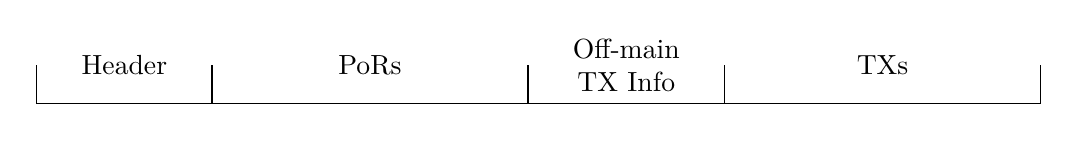
\begin{tikzpicture}[node distance=0cm]
        % \tikzstyle{n} = [draw, rectangle, solid, black, align=center, inner sep=10pt, minimum width=4cm, anchor=north]
        % \tikzstyle{tall} = [minimum height=2cm]

        % \node (header) [n] {header (\sim100 B)};
        % \node (refls) [n] at (header.south) {PoRs};
        % \node (uncles) [n] at (refls.south) {Off-main headers \\ and merkle roots};
        % \node (txs) [n] at (uncles.south) {Main TXs};
        % % \node (txs-body) [n, tall] at (refls.south) {
        % %     \node (prev-txs) [n, tall] {Sec Parents' Txs};
        % %     \node (txs) [n, tall] at (prev-txs.south) {Main Txs};
        % % };

        \tikzstyle{n} = [align=center, inner xsep=16pt, inner ysep=4pt, anchor=west]
        \tikzstyle{wide} = [minimum width=4cm]

        \node (hdr) [n] {Header};
        \node (pors) [n, wide] at (hdr.east) {PoRs};
        \node (offmain) [n] at (pors.east) {Off-main \\ TX Info};
        \node (txs) [n, wide] at (offmain.east) {TXs};

        \node (ml) at (hdr.west) {};
        \node (bl) at (offmain.south -| ml) {};
        \node (mr) at (txs.east) {};
        \node (br) at (bl -| mr) {};

        \draw (ml.center) -- (bl.center) -- (br.center) -- (mr.center);
        \draw (pors.west) -- (pors.west |- bl);
        \draw (offmain.west) -- (offmain.west |- bl);
        \draw (txs.west) -- (txs.west |- bl);

    \end{tikzpicture}
    \caption[short]{long cap}
\end{figure}

\subparagraph{Which State Roots are Accurate?}

When using a block-DAG that commits to state (e.g., a UTXO set), we've just seen that transactions in off-main blocks are only processed when they're \emph{still} valid.
For a transaction to be executed, it must be included in either a main chain block, \emph{or} an off-main block whilst not conflicting with prior transactions.

Additional  status can change between the time it's included in an off-main block and when it's executed by a main-chain block, the state root of that block

only main-chain state roots and txs are reliable.
off-main state roots are totally wrong,
and off-main transactions might be executed but we can't be sure.
only main-chain blocks and state roots matter



\subsubsubsection{Adapted NIPoPoWs for Block-DAGs: NIPoPPoWs}

\label{sec:blockdag-nipopows}
% \label{sec:nipoppows}

Recall that in \autoref{sec:nipopowrs-problem-dag-compatibility} we noted that block-DAGs are currently incompatible with NIPoPoWs.
This is because the traversal method of NIPoPoWs does not know anything about whether a block is on-main or not.
Additionally, the fork rule does not (and should not) prioritize blocks based on $\mu$ values.
So we should expect that some off-main blocks have a higher $\mu$ value than their on-main sibling and/or their first on-main descendant.
Therefore, currently, a valid NIPoPoW can lead to an off-main block -- i.e., a block that is not useful for SPV.

We do not have a problem traversing via off-main blocks, though.
They share the same cryptographic properties (with regards to interlinks) as any other block.

So, our major goal is to find a way to always arrive at on-main blocks.
A valid block-DAG NIPoPoW should never terminate at an off-main block.

One problem is that, when a block is created, the network does not know if it will be on-main or not.
Future blocks determine whether it is on-main or not.

Furthermore, we cannot be certain that all future blocks will agree that any specific block is on-main or not.
We should expect that all far-future blocks will agree, but how long should we wait and is it reliable?

Could we simply modify the interlink structure to add a flag for off-main blocks?

No -- this is not sufficient.
There is only one way (in principle) to always arrive at an on-main block: via ever more recent on-main blocks.
It is only because of an on-main block's \emph{posterity} that it becomes (and remains) on-main.
Simply flagging off-main blocks does not work because, once we reach an off-main \mu-superblock, we know nothing about which prior blocks are on-main or not.
An off-main block is (on its own) never a reliable source of prior blocks' on-main status.

% Could we take advantage of the highest common on-main ancestor?
% Theoretically, yes, if we prove enough blocks around the \mu-superblock, but providing a large block-subgraph (potentially) introduces substantial overhead, and we effectively have to do infix proofs for multiple blocks.

Here is how we can reliably arrive at on-main blocks:
first, starting from all chain-tips, we find the most recent common on-main ancestor.
If this is very close to the chain-tips, we can, instead, use an on-main ancestor a few confirmations back -- so we can meet any particular security parameter we might choose.
We can be confident that this ancestor is on-main, regardless of which chain-tip eventually ends up as the on-main block.
We must then follow the chain of primary parents.

Therefore, the interlink structure \emph{must} include enough information to traverse the $\mu$-superDAGs via on-main ancestors, only.
Just because we \emph{can} traverse via on-main blocks only does not mean that we will, though.
In fact, we will traverse via two paths: one normally, and the other via on-main blocks only.

To support this, we'll modify the interlink structure such that each link has an optional second component: the most recent on-main ancestor at that \mu level.
Most of the time, we should expect blocks to be on-main, so there will only be one interlinked entry at that \mu level.
However, in the case that a \mu-superblock is off-main, the interlink entry is both that off-main \mu-superblock, and the most recent on-main \mu-superblock (which is necessarily older than the off-main \mu-superblock).

Thus, we effectively have two \mu-superDAGs: one being the \emph{best-blocks} \mu-superDAG, and the other being the \emph{on-main only} \mu-superchain.
(Each block in a block-DAG has only one primary parent, so a chain-tip's primary ancestry really is a chain, not a DAG.)

We then construct the main suffix proof for two cases: the \emph{best-blocks} suffix proof (regardless of on-main status), and the \emph{on-main only} suffix proof.
These two proofs will always be consistent, though the best-blocks proof may not include all $\mu$-superblocks that are included in the on-main proof.
To account for this, we can require that, for each \mu level, the best-blocks \mu-superDAG suffix subgraph is a superset of the corresponding on-main \mu-superchain suffix.
Both together comprise the suffix proof.

Regarding infix proofs, we can use the existing \texttt{followDown} algorithm for with only one modification: an additional parameter determines whether \texttt{followDown} should traverse the \emph{best-blocks} path to the block, or the \emph{on-main only} path.
To generate proofs, we run \texttt{followDown} over each path.
We similarly modify the \texttt{verify-infx} (\emph{sic}) and \texttt{ancestors} functions used to verify infix proofs.
% This change requires a corresponding addition to the proof structure so that it accommodates the additional proofs that the on-main traversal requires.
% The two paths must overlap at least once: at the destination on-main block.


It is worth noting that the on-main proofs alone are not sufficient for secure NIPoPoWs: in some cases the on-main only proofs will imply substantially less total chain-weight than the best-blocks proofs.
For example: if only 50\% of blocks were on-main, then the resources an attacker needs to generate a competing NIPoPoW (for the on-main proofs) is only 50\% of what they would need compared to a best-blocks proof.
Thus, we prioritize one NIPoPoW over another based on the \emph{best-blocks} proofs (rather than the \emph{on-main} proofs).
We do, however, validate that the target of the NIPoPoW is on-main via the accompanying on-main proof.
The on-main path is only inconsistent with the best-blocks path in the case that the target block is off-main.\footnote{
    Note: when traversing the best-blocks \mu-superDAG we \emph{do not care} about the status of on-main blocks.
    Thus, the on-main interlinks in off-main \mu-superblocks are not important, and we should not count any differences there as inconsistencies with the on-main \mu-superchain.
    Similar to NIPoPoWRs, the best-blocks proof only proves that a block \emph{exists}, and no conflicts are possible via different paths.
}

A major difference between the best-blocks and on-main proofs should not be an issue for \UT{}, though, as \UT{} uses modest block frequencies for each chain.
We should expect blocks to have a single parent most of the time.
(Using the logic from \autoref{sec:por-graph-max-refl}, we'd expect simultaneous blocks \sim 2\% of the time -- give or take.)

As a final note, what happens when there are multiple paths in a \mu-superDAG?
Note that this situation only occurs in the best-blocks proof.
Since the best-blocks proof is not concerned with the posterity of blocks (their on-main status), there is no issue here.
We can choose between the paths by whichever means we like -- e.g., picking the block with the lowest PoW, or picking on-main blocks over off-main blocks when they are siblings in the same \mu-superDAG.

We've just sketched the construction of a new type of NIPoPoW that can prove \emph{both} the full chain-weight and the posterity of blocks.
The best-blocks half of the proof is almost a regular NIPoPoW on its own, but the other half of the proof (traversing on-main blocks only) is not independently secure.
However, \emph{together} they are secure.

We should distinguish between this new kind of NIPoPoW and the regular kind.
The main difference is that what we have just sketched proves \emph{work and posterity}, rather than just work.
Thus, it is a \emph{Non-Interactive Proof of Posteritorial}\footnotemark \emph{Proof of Work} (NIPoPPoW).

\footnotetext{
    A definition is require as this word is an almost-neologism: \\
    \textbf{Posteritorial} \emph{adjective}: having posterity; supported by its descendants, especially regarding well-known descendancy, explanatory antecedence, root-causal nature, etc; having a prototypical and defining quality that was widely inherited.
}




\subsubsubsection{Block-DAG Interaction With The PoR Graph}

\label{sec:dags-and-the-por-graph}

Up to now we have mostly ignored that \UT{} block-DAG simplex-chains exist within a broader context.
Particularly, we should ask: \emph{do the Axioms of \AxOfAvailability and \AxOfMaximalReflection change the game?}

Recall that, when defining the \AxiomOfMaximalReflection, we make sure to recursively include blocks' ancestors, not just reflections.
This was for two reasons.
First, \BL should not explicitly reflect its own ancestors -- links to parents \emph{are} reflections, but are the trivial case where the local and reflecting chains are the same, and the local and reflecting blocks are the same.
Second, \BL should not skip accounting for \BR's implied reflection of its parent(s), so we treat parents like any other reflected block.
We must be sure not to leave any gaps.

There is still one gap, though: \cL blocks that are not an ancestor of \BL.

It should be clear that parent links are qualitatively different from reflections: child blocks attest to the validity of their parent blocks, and to continuity between these two blocks.
% This was the reason for the predicate's (ii)(b) condition
``PoR'' between these blocks is also free, unlike explicit PoRs between blocks of different chains.

Unlike traditional chains, \UT{} blocks are not only allowed to have multiple parents, but \emph{can always include a valid block as an ancestor}.
Recall the \AxiomOfMaximalReflection's principle: \emph{\PrincipleOfMaximalReflection} % space but no full stop
Considering the symmetry between parents and reflected blocks, we can devise a new principle: \emph{A miner should build on all possible chain-tips.}

In effect, we want to ensure that a dishonest miner cannot evade the contradiction in refusing to build on a valid chain-tip whilst acknowledging it as available.
If it is unavailable then the miner should not reflect the blocks that imply it is available; and if it is available and valid then it should be a parent of their draft block.

So far, this principle is fine for honest miners building on \emph{valid} blocks -- including every chain-tip as a parent is what we expect honest miners to do by default.
However, what are honest miners to do if there is an invalid block?

We already know enough to answer this, of course: link back to, or \emph{flag}, that block as invalid with an attached fraud proof, and never use that block as a parent.
The transactions in that block aren't important, so we don't care about keeping them --- the offending transaction is part of the fraud proof in any case.
And we can reconstruct the PoRs sub-block using $O(1)$ data thanks to \AxOfMaximalReflection.
Thus, an invalid block is only as large as its header, list of reflected PoR graph-tips, and fraud proof.
That's $O(\log c)$ in the worst case.

% It is only in the case of an invalid block that it cannot be an ancestor, and in that case the miner \emph{must} link to it with the fraud proof attached.
% This link is sort of like a reflection, but it comes with a note saying \emph{this block will never be valid, and here's why}.
% Since the transactions within such a block are non-canonical, we don't count it as an ancestor.
% Thus, the entire PoR graph learns that the block is invalid.

\subsubsubsection{\AxiomOfRawUnifiedAncestry}

\DeclareAxiom{UnifiedAncestry}{
    A miner should use all valid chain-tips as parents, and flag invalid ones.
}{
    A block, \BL{}, is invalid unless, for all reflected blocks \BR{}:
    \begin{axiomreqs}
        \item \BR{} is valid under this axiom; and
        \item each \cL block reflected by \BR{}:
        \begin{enumerate}[label=\alph*.]
            \item is an ancestor of \BL{}; or
            % \item shares no ancestors with \BL; or
            \item is flagged as invalid by \BL{}; or
            \item was flagged as invalid by an ancestor of \BL{}.
        \end{enumerate}
    \end{axiomreqs}
}

This new axiom changes the game for block-DAGs.
Previously, an attacker could delay transactions for $\sim {A_\text{blocks}}^2$ many blocks because they could evade the contradiction in the PoR graph.
Now, they cannot.
Thus, empty block DoS attacks against simplex-chain block-DAGs are limited to $\sim A_\text{blocks}$ in length (on average).\footnote{
    We will reduce this further in \autoref{sec:miner-resonance}.
}
In terms of DoS potential, this is \emph{exactly} the same as if the simplex-chain were a traditional chain and the attacker always built on the best block, but only made empty blocks.
Now that we've added the \AxiomOfUnifiedAncestry, the alternative for the attacker is producing only invalid blocks.

\aside{
    Note that this axiom applies in the context of the PoR graph rather than local chain-state.\\
    The entire PoR graph learns of and verifies the fraud proof.
}

\subsubsubsection{NIPoPPoWs + NIPoPoWRs = NIPoPPoWaPoWRs}

In \autoref{sec:blockdag-nipopows} we devised NIPoPPoWs, modified NIPoPoWs that work with block-DAGs by accounting for posterity.
That construction depended a \emph{best-blocks} proof in combination with an \emph{on-main only} proof.
In the case of simplex-chain block-DAGs, we do not want to use the same best-blocks proof as it only accounts for local chain-work and does not include reflections.

Instead of a standard best-blocks NIPoPoWs, we can use NIPoPoWRs from \autoref{sec:nipopowrs}.
Functionally, both serve the same purpose: proving that a block \emph{exists}.

However, the best-blocks proof had substantial overlap with the on-main only proof -- that isn't the case for NIPoPoWRs as \emph{most} of the \mu-superblocks will be from reflecting chains.
Rater, we expect the best posteritorial \mu-superchain to have a \mu level approximately $\log_2({N_1})$ lower than that of the best PoR \mu-superDAG.



\subsubsubsubsection{Integrating Fraud Proofs}




% 
\subsubsubsection{Preventing DoS Attacks}

\label{sec:preventing-dos-attacks}

Consider the situation where an attacker is attempting to deny service via the production of empty blocks, and that the attacker can create blocks faster than the honest network.
Such a situation is illustrated in \autoref{fig:dag-dos-1}.
Since the goal of the attack is to prevent transactions from occurring, the attacker must\footnote{
    The attacker could also fill the blocks with spam transactions.
    That's more work for the attacker, but also more work for the honest network (calculating and storing that state, maybe indefinitely).
    It's preferable that the attacker has minimal transactions in their blocks.
    It's tempting to think of ideas like: \emph{since the attacker's blocks are empty, we can let honest nodes make larger blocks via some kind of weighted average block size calculation plus some flexibility in the size of blocks produced}.
    The problem with this is that it incents the attacker to fill their blocks with spam transactions, which is counterproductive.
} produce empty\footnote{
    Note that the attacker should still be reflecting other simplex-chains so as to maximize the total weight of the attacker's chain-segment.
    Given this, the attacker's blocks will contain reflected simplex-chain headers but no transactions.
} blocks.
Furthermore, if the attacker links back to any honest blocks then the honest blocks' histories will be merged with the canonical history; thus the attack would fail.
The attacker's only available strategy is to produce a single chain of empty blocks.


\begin{figure}[ht]
    \centering
    \includegraphics[width=\linewidth]{dag_dos_v2_sag}
    \caption[
        An attempted empty-block DoS attack on a block-DAG.
    ]{
        An attempted empty-block DoS attack on a block-DAG.
        The attacker's blocks, $A_{i+\_}$, are mined in public and contain no transactions.
        Each block is annotated with its \emph{chain-weight} ($\Sigma_w$); a double outline indicates that a block is part of the main chain.
        Even though the attacker produces $2\times$ as many blocks as the honest network, the attack inevitably fails after a short while.
        Note: $H_i$ is defined to have $\Sigma_w = 0$ for illustrative convenience.
    }
    \label{fig:dag-dos-1}
\end{figure}

How does such an attack fair?
The challenge of such a DoS attack is to prevent honest miners from extending the attacker's chain-segment.
For traditional (non-DAG) chains --- where each non-genesis block has exactly one parent --- this is accomplished as soon as the attacker is able to reliably produce a heavier chain-segment than the honest network for a given period.\footnote{
    For a traditional blockchain, this would also imply a 51\% attack, so this isn't a situation that those chains have to deal with.
    In a simplex, however, a miner can have $>50\%$ of a chain's local hash-rate, so we need to handle this case.
}
% <!-- (Typically, this means the attacker produces blocks more frequently.) -->

However, if blocks are allowed to have \emph{more} than one parent then there \emph{is no point} where an attacker can \emph{maintain} a DoS attack indefinitely.
Instead, they can only \emph{delay the execution} of some transactions for a short period of time.
Particularly, if an attacker can produce $A_{\text{blocks}} > 1$ for every 1 block produced by the honest network, then the attack can delay honest transactions for up to approximately $({A_{\text{blocks}}}^2 - 1) \cdot {B_f}^{-1}$ seconds, where $B_f$ is the frequency of block production (in Hz).
After this (approximate) point, the weight of the honest chain-segment, which includes the attacker's chain-segment, is always greatest.

If an attacker performs a \emph{repeating cycle} of these attacks, then they may be able to decrease the effective capacity of the chain by a factor of ${A_{\text{blocks}}}^2$. %<!-- / (1 + A_{\text{blocks}}) -->
The opportunity cost of this attack, for the attacker, is at least as much as the lost transaction fees.
% <!-- note: with the distance from the main/pivot chain penalty in "Inclusive Block Chain Protocols", a smaller attacker isn't penalized much, but a larger attacker is penalized a lot WRT block rewards -->

All that sounds okay so far (maybe not that last bit), but this thought experiment is flawed.
It is \emph{smoothed out} compared to what we'd expect in reality --- the discrete and probabilistic natures of block production and reflections are ignored.
In \autoref{fig:dag-dos-1}, those are explicitly excluded!
What happens if we include the effect of other simplex-chains, though?
% Well... something \emph{magical}.

\todoDraftOnly{As soon as an honest block is created linking back to a most-recent attacker block, the game is over.}

Consider an attacker producing 2 blocks for every 1 honest block.
What happens most of the time?
Well the attacker's blocks get reflected first, so those blocks have an appreciable advantage over the honest blocks.
The honest blocks will get reflected, too, but most of the time the attacker's blocks will get the advantage from earlier reflections.
\emph{Most} of the time.
Occasionally, when an honest block is a bit lucky, an honest block will beat the attacker's next block --- gaining reflections earlier.
At that point, the attacker has lost --- they need to outpace the \emph{difference} in the number of reflections between the honest block and attacking blocks.
So, unlike a normal doublespend (where the attacker wins if they \emph{ever} get ahead), now the honest network wins (ends the DoS) if it \emph{ever} gets ahead of the attacker --- after that point, there's no viable strategy for the attacker besides to build on the honest blocks.
\emph{The asymmetry has flipped!}

\begin{comment}
- mk
cut from after "when an honest block is a bit lucky":
> (which will be more often if there's \emph{miner resonance})
it's worth noting the convergence better than we do atm (right now, that's: "If there were, it'd be possible to temporarily limit the attacker to $<50\%$ of mining power, ending the DoS quickly. (See \autoref{sec:miner-resonance}.))"
\end{comment}

\todoDraftOnly{
    Analyze including requirement to only reflect extant data.
    This means that the chain-tips get the weight (advantage honest b/c H builds on A blocks and H blocks).
    Attacker blocks lose out on PoRs but honest chain includes all PoRs.
    the attacker might lie about the requirement and be okay with reflecting non-extant data, but then other chains won't reflect it.
}

There's more that can be done here, too, like honest users creating transactions (with large fees) that depend on certain history (i.e., that some honest block is in the history of the chain).
That will attract miners from other chains due to unrealized RoI (potentially a lot).
The attacker could include that transaction, but then they need to voluntarily end the DoS themselves.
If you're worried about that, because it seems like miners might empty-block DoS simplex-chains, consider: when in equilibrium, that situation is essentially the same as an efficient market (for transaction execution).

\todoDraftOnly{Is it essentially the same?}

Is there a reasonable strategy whereby the honest network can temporarily increase the number of miners?
If there were, it'd be possible to temporarily limit the attacker to $<50\%$ of mining power, ending the DoS quickly.
(See \autoref{sec:miner-resonance}.)



\todoDraftOnly{The above should work for simplex-chains \emph{and} dapp-chains}

\todoDraftOnly{Dynamic average block-size for simplex-chains based on dapp-chain headers having some PoW}

% \subsubsubsection{Merging Histories}

\todo{merging histories}

\def\blkGrp#1{\save [].[r]!C="g#1"*[F.]\frm{}\restore}%
\def\blkGrpM[#1]#2{\save [].[#1]!C="g#2"*[F.]\frm{}\restore}%

\subparagraph{simple}

\begin{equation*}
    \xyMChains{
        & & & \xBB{1a} \arm[ld] & & \xBB{2a} \arm[ll] \\
        & \cdots & \xBBi \arm[l] & & & & \xBB3 \arm[lu] \ars[lld] \\
        & & & & \xBB{1b} \arm[llu] & \\
        & \xyTimeHoriz{rrrrrr} &&&&&&
    }
\end{equation*}

\begin{equation*}
    \xyMChains{
        % & & & \xBB{1a} \arm[ld] & & \xBB{2a} \arm[ll] \\
        & \cdots \arm[r]
            & \xBBi \arm[r]
            & \xBB{1a} \arm[r]
            & \xBB{2a} \arm[r]
            & \xyBDraft{\BB{1b}} \arm[r] \blkGrp1
            & \xBB3 \\
        & \xyLabelHoriz{Execution Order}{0pt}{rrrrrr}{r30pt} &&&&&&
        % \save "1,6"."1,7"*[F.]\frm{}
        % \restore
    }
\end{equation*}

\subparagraph{bit complex}

\begin{equation*}
    \xyMChains{
        & & & \xBB{1a} \arm[ld] & \xBB{2a} \arm[l] \ars[ldd] \\
        & \cdots & \xBBi \arm[l] & & & & \xBB3 \arm[llu] \ars[ld] \\
        & & & \xBB{1b} \arm[lu] & & \xBB{2b} \ars[ll] \arm[lluu] \\
        & \xyTimeHoriz{rrrrrr} &&&&&&
    }
\end{equation*}

\begin{equation*}
    \xyMChains{
        & \cdots \arm[r]
            & \xBBi \arm[r]
            & \xBB{1a} \arm[r]
            & \xyBDraft{\BB{1b}} \arm[r] \blkGrp1
            & \xBB{2a} \arm[r]
            & \xyBDraft{\BB{2b}} \arm[r] \blkGrp2
            & \xBB3 \\
        & \xyLabelHoriz{Execution Order}{0pt}{rrrrrr}{r30pt} &&&&&&
    }
\end{equation*}

\subparagraph{multiparent}

\begin{equation*}
    \xyMChains{
        & & & & \xBB{2a} \arm[ld] \\
        & \cdots & \xBBi \arm[l] & \xBB{1} \arm[l] & \xBB{2b} \arm[l] & \xBB3 \arm[lu]_1 \ars[l]_2 \ars[ld]^3 \\
        & & & & \xBB{2c} \arm[lu] \\
        & \xyTimeHoriz{rrrrrr} &&&&&&
    }
\end{equation*}

\begin{equation*}
    \xyMChains{
        & \cdots \arm[r]
            & \xBBi \arm[r]
            & \xBB{1} \arm[r]
            & \xBB{2a} \arm[r]
            & \xyBDraft{\BB{2b}} \arm[r] \blkGrpM[rr]1
            & \xyBDraft{\BB{2c}} \arm[r]
            & \xBB3 \\
        & \xyLabelHoriz{Execution Order}{0pt}{rrrrrr}{r30pt} &&&&&&
    }
\end{equation*}

\subparagraph{block structure}

\begin{figure}
    \centering
    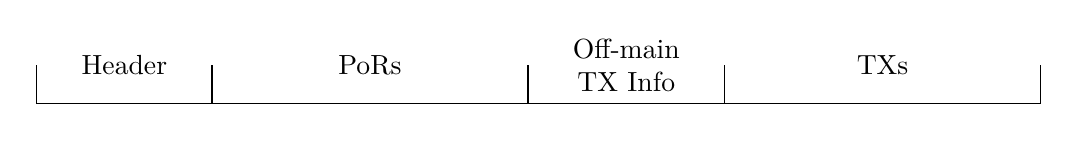
\begin{tikzpicture}[node distance=0cm]
        % \tikzstyle{n} = [draw, rectangle, solid, black, align=center, inner sep=10pt, minimum width=4cm, anchor=north]
        % \tikzstyle{tall} = [minimum height=2cm]

        % \node (header) [n] {header (\sim100 B)};
        % \node (refls) [n] at (header.south) {PoRs};
        % \node (uncles) [n] at (refls.south) {Off-main headers \\ and merkle roots};
        % \node (txs) [n] at (uncles.south) {Main TXs};
        % % \node (txs-body) [n, tall] at (refls.south) {
        % %     \node (prev-txs) [n, tall] {Sec Parents' Txs};
        % %     \node (txs) [n, tall] at (prev-txs.south) {Main Txs};
        % % };

        \tikzstyle{n} = [align=center, inner xsep=16pt, inner ysep=4pt, anchor=west]
        \tikzstyle{wide} = [minimum width=4cm]

        \node (hdr) [n] {Header};
        \node (pors) [n, wide] at (hdr.east) {PoRs};
        \node (offmain) [n] at (pors.east) {Off-main \\ TX Info};
        \node (txs) [n, wide] at (offmain.east) {TXs};

        \node (ml) at (hdr.west) {};
        \node (bl) at (offmain.south -| ml) {};
        \node (mr) at (txs.east) {};
        \node (br) at (bl -| mr) {};

        \draw (ml.center) -- (bl.center) -- (br.center) -- (mr.center);
        \draw (pors.west) -- (pors.west |- bl);
        \draw (offmain.west) -- (offmain.west |- bl);
        \draw (txs.west) -- (txs.west |- bl);

    \end{tikzpicture}
    \caption[short]{long cap}
\end{figure}

\subparagraph{Which State Roots are Accurate?}

When using a block-DAG that commits to state (e.g., a UTXO set), we've just seen that transactions in off-main blocks are only processed when they're \emph{still} valid.
For a transaction to be executed, it must be included in either a main chain block, \emph{or} an off-main block whilst not conflicting with prior transactions.

Additional  status can change between the time it's included in an off-main block and when it's executed by a main-chain block, the state root of that block

only main-chain state roots and txs are reliable.
off-main state roots are totally wrong,
and off-main transactions might be executed but we can't be sure.
only main-chain blocks and state roots matter

% 
\subsubsubsection{Adapted NIPoPoWs for Block-DAGs: NIPoPPoWs}

\label{sec:blockdag-nipopows}
% \label{sec:nipoppows}

Recall that in \autoref{sec:nipopowrs-problem-dag-compatibility} we noted that block-DAGs are currently incompatible with NIPoPoWs.
This is because the traversal method of NIPoPoWs does not know anything about whether a block is on-main or not.
Additionally, the fork rule does not (and should not) prioritize blocks based on $\mu$ values.
So we should expect that some off-main blocks have a higher $\mu$ value than their on-main sibling and/or their first on-main descendant.
Therefore, currently, a valid NIPoPoW can lead to an off-main block -- i.e., a block that is not useful for SPV.

We do not have a problem traversing via off-main blocks, though.
They share the same cryptographic properties (with regards to interlinks) as any other block.

So, our major goal is to find a way to always arrive at on-main blocks.
A valid block-DAG NIPoPoW should never terminate at an off-main block.

One problem is that, when a block is created, the network does not know if it will be on-main or not.
Future blocks determine whether it is on-main or not.

Furthermore, we cannot be certain that all future blocks will agree that any specific block is on-main or not.
We should expect that all far-future blocks will agree, but how long should we wait and is it reliable?

Could we simply modify the interlink structure to add a flag for off-main blocks?

No -- this is not sufficient.
There is only one way (in principle) to always arrive at an on-main block: via ever more recent on-main blocks.
It is only because of an on-main block's \emph{posterity} that it becomes (and remains) on-main.
Simply flagging off-main blocks does not work because, once we reach an off-main \mu-superblock, we know nothing about which prior blocks are on-main or not.
An off-main block is (on its own) never a reliable source of prior blocks' on-main status.

% Could we take advantage of the highest common on-main ancestor?
% Theoretically, yes, if we prove enough blocks around the \mu-superblock, but providing a large block-subgraph (potentially) introduces substantial overhead, and we effectively have to do infix proofs for multiple blocks.

Here is how we can reliably arrive at on-main blocks:
first, starting from all chain-tips, we find the most recent common on-main ancestor.
If this is very close to the chain-tips, we can, instead, use an on-main ancestor a few confirmations back -- so we can meet any particular security parameter we might choose.
We can be confident that this ancestor is on-main, regardless of which chain-tip eventually ends up as the on-main block.
We must then follow the chain of primary parents.

Therefore, the interlink structure \emph{must} include enough information to traverse the $\mu$-superDAGs via on-main ancestors, only.
Just because we \emph{can} traverse via on-main blocks only does not mean that we will, though.
In fact, we will traverse via two paths: one normally, and the other via on-main blocks only.

To support this, we'll modify the interlink structure such that each link has an optional second component: the most recent on-main ancestor at that \mu level.
Most of the time, we should expect blocks to be on-main, so there will only be one interlinked entry at that \mu level.
However, in the case that a \mu-superblock is off-main, the interlink entry is both that off-main \mu-superblock, and the most recent on-main \mu-superblock (which is necessarily older than the off-main \mu-superblock).

Thus, we effectively have two \mu-superDAGs: one being the \emph{best-blocks} \mu-superDAG, and the other being the \emph{on-main only} \mu-superchain.
(Each block in a block-DAG has only one primary parent, so a chain-tip's primary ancestry really is a chain, not a DAG.)

We then construct the main suffix proof for two cases: the \emph{best-blocks} suffix proof (regardless of on-main status), and the \emph{on-main only} suffix proof.
These two proofs will always be consistent, though the best-blocks proof may not include all $\mu$-superblocks that are included in the on-main proof.
To account for this, we can require that, for each \mu level, the best-blocks \mu-superDAG suffix subgraph is a superset of the corresponding on-main \mu-superchain suffix.
Both together comprise the suffix proof.

Regarding infix proofs, we can use the existing \texttt{followDown} algorithm for with only one modification: an additional parameter determines whether \texttt{followDown} should traverse the \emph{best-blocks} path to the block, or the \emph{on-main only} path.
To generate proofs, we run \texttt{followDown} over each path.
We similarly modify the \texttt{verify-infx} (\emph{sic}) and \texttt{ancestors} functions used to verify infix proofs.
% This change requires a corresponding addition to the proof structure so that it accommodates the additional proofs that the on-main traversal requires.
% The two paths must overlap at least once: at the destination on-main block.


It is worth noting that the on-main proofs alone are not sufficient for secure NIPoPoWs: in some cases the on-main only proofs will imply substantially less total chain-weight than the best-blocks proofs.
For example: if only 50\% of blocks were on-main, then the resources an attacker needs to generate a competing NIPoPoW (for the on-main proofs) is only 50\% of what they would need compared to a best-blocks proof.
Thus, we prioritize one NIPoPoW over another based on the \emph{best-blocks} proofs (rather than the \emph{on-main} proofs).
We do, however, validate that the target of the NIPoPoW is on-main via the accompanying on-main proof.
The on-main path is only inconsistent with the best-blocks path in the case that the target block is off-main.\footnote{
    Note: when traversing the best-blocks \mu-superDAG we \emph{do not care} about the status of on-main blocks.
    Thus, the on-main interlinks in off-main \mu-superblocks are not important, and we should not count any differences there as inconsistencies with the on-main \mu-superchain.
    Similar to NIPoPoWRs, the best-blocks proof only proves that a block \emph{exists}, and no conflicts are possible via different paths.
}

A major difference between the best-blocks and on-main proofs should not be an issue for \UT{}, though, as \UT{} uses modest block frequencies for each chain.
We should expect blocks to have a single parent most of the time.
(Using the logic from \autoref{sec:por-graph-max-refl}, we'd expect simultaneous blocks \sim 2\% of the time -- give or take.)

As a final note, what happens when there are multiple paths in a \mu-superDAG?
Note that this situation only occurs in the best-blocks proof.
Since the best-blocks proof is not concerned with the posterity of blocks (their on-main status), there is no issue here.
We can choose between the paths by whichever means we like -- e.g., picking the block with the lowest PoW, or picking on-main blocks over off-main blocks when they are siblings in the same \mu-superDAG.

We've just sketched the construction of a new type of NIPoPoW that can prove \emph{both} the full chain-weight and the posterity of blocks.
The best-blocks half of the proof is almost a regular NIPoPoW on its own, but the other half of the proof (traversing on-main blocks only) is not independently secure.
However, \emph{together} they are secure.

We should distinguish between this new kind of NIPoPoW and the regular kind.
The main difference is that what we have just sketched proves \emph{work and posterity}, rather than just work.
Thus, it is a \emph{Non-Interactive Proof of Posteritorial}\footnotemark \emph{Proof of Work} (NIPoPPoW).

\footnotetext{
    A definition is require as this word is an almost-neologism: \\
    \textbf{Posteritorial} \emph{adjective}: having posterity; supported by its descendants, especially regarding well-known descendancy, explanatory antecedence, root-causal nature, etc; having a prototypical and defining quality that was widely inherited.
}

% 

\subsubsubsection{Block-DAG Interaction With The PoR Graph}

\label{sec:dags-and-the-por-graph}

Up to now we have mostly ignored that \UT{} block-DAG simplex-chains exist within a broader context.
Particularly, we should ask: \emph{do the Axioms of \AxOfAvailability and \AxOfMaximalReflection change the game?}

Recall that, when defining the \AxiomOfMaximalReflection, we make sure to recursively include blocks' ancestors, not just reflections.
This was for two reasons.
First, \BL should not explicitly reflect its own ancestors -- links to parents \emph{are} reflections, but are the trivial case where the local and reflecting chains are the same, and the local and reflecting blocks are the same.
Second, \BL should not skip accounting for \BR's implied reflection of its parent(s), so we treat parents like any other reflected block.
We must be sure not to leave any gaps.

There is still one gap, though: \cL blocks that are not an ancestor of \BL.

It should be clear that parent links are qualitatively different from reflections: child blocks attest to the validity of their parent blocks, and to continuity between these two blocks.
% This was the reason for the predicate's (ii)(b) condition
``PoR'' between these blocks is also free, unlike explicit PoRs between blocks of different chains.

Unlike traditional chains, \UT{} blocks are not only allowed to have multiple parents, but \emph{can always include a valid block as an ancestor}.
Recall the \AxiomOfMaximalReflection's principle: \emph{\PrincipleOfMaximalReflection} % space but no full stop
Considering the symmetry between parents and reflected blocks, we can devise a new principle: \emph{A miner should build on all possible chain-tips.}

In effect, we want to ensure that a dishonest miner cannot evade the contradiction in refusing to build on a valid chain-tip whilst acknowledging it as available.
If it is unavailable then the miner should not reflect the blocks that imply it is available; and if it is available and valid then it should be a parent of their draft block.

So far, this principle is fine for honest miners building on \emph{valid} blocks -- including every chain-tip as a parent is what we expect honest miners to do by default.
However, what are honest miners to do if there is an invalid block?

We already know enough to answer this, of course: link back to, or \emph{flag}, that block as invalid with an attached fraud proof, and never use that block as a parent.
The transactions in that block aren't important, so we don't care about keeping them --- the offending transaction is part of the fraud proof in any case.
And we can reconstruct the PoRs sub-block using $O(1)$ data thanks to \AxOfMaximalReflection.
Thus, an invalid block is only as large as its header, list of reflected PoR graph-tips, and fraud proof.
That's $O(\log c)$ in the worst case.

% It is only in the case of an invalid block that it cannot be an ancestor, and in that case the miner \emph{must} link to it with the fraud proof attached.
% This link is sort of like a reflection, but it comes with a note saying \emph{this block will never be valid, and here's why}.
% Since the transactions within such a block are non-canonical, we don't count it as an ancestor.
% Thus, the entire PoR graph learns that the block is invalid.

\subsubsubsection{\AxiomOfRawUnifiedAncestry}

\DeclareAxiom{UnifiedAncestry}{
    A miner should use all valid chain-tips as parents, and flag invalid ones.
}{
    A block, \BL{}, is invalid unless, for all reflected blocks \BR{}:
    \begin{axiomreqs}
        \item \BR{} is valid under this axiom; and
        \item each \cL block reflected by \BR{}:
        \begin{enumerate}[label=\alph*.]
            \item is an ancestor of \BL{}; or
            % \item shares no ancestors with \BL; or
            \item is flagged as invalid by \BL{}; or
            \item was flagged as invalid by an ancestor of \BL{}.
        \end{enumerate}
    \end{axiomreqs}
}

This new axiom changes the game for block-DAGs.
Previously, an attacker could delay transactions for $\sim {A_\text{blocks}}^2$ many blocks because they could evade the contradiction in the PoR graph.
Now, they cannot.
Thus, empty block DoS attacks against simplex-chain block-DAGs are limited to $\sim A_\text{blocks}$ in length (on average).\footnote{
    We will reduce this further in \autoref{sec:miner-resonance}.
}
In terms of DoS potential, this is \emph{exactly} the same as if the simplex-chain were a traditional chain and the attacker always built on the best block, but only made empty blocks.
Now that we've added the \AxiomOfUnifiedAncestry, the alternative for the attacker is producing only invalid blocks.

\aside{
    Note that this axiom applies in the context of the PoR graph rather than local chain-state.\\
    The entire PoR graph learns of and verifies the fraud proof.
}

\subsubsubsection{NIPoPPoWs + NIPoPoWRs = NIPoPPoWaPoWRs}

In \autoref{sec:blockdag-nipopows} we devised NIPoPPoWs, modified NIPoPoWs that work with block-DAGs by accounting for posterity.
That construction depended a \emph{best-blocks} proof in combination with an \emph{on-main only} proof.
In the case of simplex-chain block-DAGs, we do not want to use the same best-blocks proof as it only accounts for local chain-work and does not include reflections.

Instead of a standard best-blocks NIPoPoWs, we can use NIPoPoWRs from \autoref{sec:nipopowrs}.
Functionally, both serve the same purpose: proving that a block \emph{exists}.

However, the best-blocks proof had substantial overlap with the on-main only proof -- that isn't the case for NIPoPoWRs as \emph{most} of the \mu-superblocks will be from reflecting chains.
Rater, we expect the best posteritorial \mu-superchain to have a \mu level approximately $\log_2({N_1})$ lower than that of the best PoR \mu-superDAG.



\subsubsubsubsection{Integrating Fraud Proofs}


\subsection{SPV}

% right above this is label: sec:spv-in-ut

\subsubsection{Introduction}

Our goal in this section is to find a method for cross-chain transactions between any two simplex-chains that is safe, fast, succinct, and reliable.
\begin{itemize}
    \item \emph{Safe}: an adversary must perform a 51\% attack to execute an invalid cross-chain transaction.
    \item \emph{Fast}: $O(t) \le O(\lambda) = O(1)$, where: $t$ is the maximum delay between a cross-chain transaction being confirmed by a simplex-chain and the point at which the destination simplex-chain allows processing that transaction; $\lambda$ is a security parameter (e.g., $\lambda = 4$ local confirmations).
    \item \emph{Succinct}: for any cross-chain proof $\pi$, $O(\pi) < O(c)$ and $|\pi|$ is practical.
    \item \emph{Reliable}: the above properties hold for all transactions in all simplex-chains.
\end{itemize}

Given everything we have discussed up to now, it's not clear how cross-chain transactions are possible.
The problem is that miners on one simplex-chain do not validate the state transitions of other simplex-chains.
Each simplex-chain, locally, has an $O(\nicefrac{n}{c})$ share of the network's security (assuming there are $O(c)$ many chains).
An $O(\nicefrac{n}{c})$ adversary could theoretically produce \emph{all} of the blocks for a single simplex-chain (e.g., by mining at a slight loss to push other miners out).
The adversary could then create a very long chain of blocks that have valid headers, PoRs, etc, but also contain one or more fraudulent transactions.
Perhaps the main chain eventually corrects to a non-fraudulent history (similar to \autoref{sec:preventing-dos-attacks}) --- but in that case we'd need to wait a \emph{very} long time to be sure that such a correction \emph{must} have happened.
That violates the \emph{fast} goal, so this eventual-correction idea fails to meet our overall goal.

Are we stuck?
For a blockchain network to be scalable, it must be the case that miners are \emph{not} required to validate more than one chain!
Have we come all this way, attempting to deal with the core conflict of the trilemma, only to find that we just moved the conflict?

\subsubsection{Why does SPV work for Bitcoin?}

For the sake of simplicity, let's consider Bitcoin in isolation.
Particularly, we'll assume that there are no other networks of similar size using the same PoW algorithm or compatible mining hardware.

A concise argument for the security of Bitcoin-SPV proofs is:

\begin{argumentslist}
    \item An SPV proof is a merkle branch proving that a transaction exists in a block.
    \item All blocks are part of the same blockchain and history.
    \item All transactions that occur are in some block's merkle tree.
    \item If a transaction is invalid, then the block is invalid.
    \item If a block builds on an invalid block, then it is invalid.
    \item If a miner produces an invalid block, they get no block reward.
    \item $\implies$ Honest miners won't produce or build on invalid blocks.
    \item \label{prem:spv-7} $\implies$ For an adversary to produce an apparently valid (but fraudulent) proof leading to a \emph{main chain} block, they'd need to out-compete honest miners (i.e., 51\% attack the network).
    \item \label{prem:spv-8} $\implies$ Only valid transactions exist in the main chain.\footnote{
        This isn't the full picture for some blockchains (e.g., Ethereum), even though SPV still works for them --- a transaction that fails to execute can still be valid and produce a valid state transition.
        In these cases, an invalid state transition implies an invalid block, so it's customary to prove that some state has the right values rather than that a transaction exists.
    }
    \item $\implies$ It's safe to accept SPV proofs for blocks in the main chain.
\end{argumentslist}

It appears that \cref{prem:spv-7} is our current sticking point for Simplex-SPV proofs.

But, we don't necessarily \emph{need} to replicate \cref{prem:spv-7} if we could get to \cref{prem:spv-8} by other means.

\subsubsection{Method}

\infoNote{
    The details below are an overview of Amaroo's cross-chain protocol.
    Full details comprise the Amaroo team's forthcoming paper on the subject.
}

\subsubsubsection{Context}

The purpose of UT's cross-chain protocol is to \emph{maintain coherence} between simplex-chains.
This means that all the essential properties we'd expect to hold for transactions on a single chain should hold between chains, too: coins are not created nor destroyed\footnote{
    That isn't to say burning coins isn't possible, but it should never be an unintended byproduct of a cross-chain transaction.
}, coins can only be spent once, \emph{the transaction executes entirely or not at all}, etc.
There will obviously be some particular properties that are different, such as a delay between inputs being spent (on the sending chain) and outputs being created (on the receiving chain).



\begin{comment}
    - hard things
      - guaranteed execution vs guaranteed to be redeemable

    - if a tx is valid, then spending the same inputs with a cross-chain wrapper around the outputs is valid
    - the validity of a transaction is evaluated and enforced entirely on the sending chain
    - if a transaction is invalid, then a fraud proof is possible
    - the \AxiomOfAvailability means miners on the receiving chain can easily find all incoming XC transactions
    - if a fraud proof exists for a block, then the block is invalid
    - a fraud proof can be included by any miner from any simplex chain (and goes in the PoR graph)
    - if a block is invalid, then all blocks of that chain that build on it are invalid
    - if a block is invalid, reflecting blocks are not immediately invalidated
    - however, reflecting blocks outside the security parameter are invalid \emph{unless} they build on PoR graph tips that include the fraud proof


    - normal SPV is PUSH-PULL: you PUSH on the sending chain and PULL on the receiving chain
    - We can do PUSH-PUSH: you PUSH on the sending chain it is automatically PUSHed on the receiving chain
    - We can also do PULL-PUSH: you PULL on the receiving chain, which automatically PUSHes on the sending chain to the receiving chain
      - this requires an output type: SpendIfExistsElse which tests whether an output exists and then produces one of two outcomes depending on the result
      - you send that PUSH-PUSH style from a chain, which then auto-execs the output on the receiving chain. If the exists branch is an XC output, then this is also PUSH-PUSH. So it functions as PULL-PUSH.
    - Our cases require only 1 tx compared to the typical 2 txs.



- DoS issue
- Bribe issue
- Decoherence (mint funds)

% important: censorship resistance
\end{comment}


% -- context

Before we address how cross-chain transactions will work, we first need to remember the context in which we're operating.
Leading up to this point, we've constructed a network with some wildly different properties to traditional blockchains: ultra-fast confirmations, additional DoS and censorship resistance, shared security, higher order scaling, etc.
These improvements are due to the specific combination of: \emph{Proof of Reflection}, the use of chain-like block-DAGs in the PoR Graph and each simplex-chain, and the Axioms of \AxOfAvailability{}, \AxOfMaximalReflection{}, and \AxOfUnifiedAncestry{}.
Each of these ideas, along with fraud proofs, will have a role to play in the cross-chain protocol described shortly.

Additionally, we are concerned about some possible attacks aimed at the cross-chain protocol.
We are not necessarily concerned about how the protocol resolves during a 51\% attack in this discussion since we already know that the network does not function in that context.

The first and most important thing to consider is \emph{Under which circumstances can cross-chain transactions be invalidated?}
If it is possible to invalidate a past cross-chain transaction, this could be used to perform a doublespend, or coin duplication, etc.
Therefore, we should strive for a protocol that only permits such invalidation under a 51\% attack (or worse).
That way, we can be confident that the cross-chain protocol is not the weakest link in the chain, since local (intra-chain) transactions break down at that point, anyway.

The obvious way to invalidate a cross-chain transaction is to cause a reorganization on the origin chain.
If the pivot of the reorganization is antecedent to the cross-chain transaction, then it is up to the attacker whether that transaction is included in the resulting canonical history.
This outcome is self-evidently insecure.
Therefore our question about cross-chain transaction invalidation has the same answer as questions like \emph{Under which circumstances can a simplex-chain reorganization occur?}
We are also concerned with the parameters around such a reorganization: \emph{Is it dependent on the number of confirmations?}, \emph{If so, how many?}, \emph{What proportion of global hash-rate is required?}, etc.

Fortunately, we've done a lot of the legwork already to prove that the ordering of simplex-chain blocks is stable and works for cross-chain transactions.
\emph{Proof of Reflection} allows us to share security between simplex-chains.
Block-DAGs and the PoR Graph provide some censorship resistance, and more importantly, are the basis for both the \AxiomOfMaximalReflection{} and the \AxiomOfUnifiedAncestry{}.
These axioms go on to, respectively, bind the histories of each simplex-chain to one another and ensure that each chain's history spans all valid blocks of that chain in the PoR graph.
The binding of histories is the basis for the \emph{coherence} of the simplex, and PoR graph-spanning histories ensures that the ordering of blocks within each chain conforms to the ordering of blocks in the PoR graph.
Therefore: to change the order of blocks within a simplex-chain requires that an attacker change the global ordering, which in turn requires a 51\% attack.
$\blacksquare$

Regarding network security, resisting this particular attack is paramount because this kind of reorganization \emph{affects honest nodes}.
By comparison, there are other attacks that do not affect honest nodes, but do affect, say, light clients.\footnote{
    In this context light clients are not considered honest nodes (nor attacking nodes) since they do not contribute to global consensus.
}
These other attacks aren't as concerning provided that they only affect non-validating network participants.
But! What happens when an invalid block is mined?
It \emph{will} be reflected, because miners of other simplex-chains do not validate the block.
What we need is a method of \emph{error correction} -- one that is fast enough to ensure invalid blocks are dealt with before the cross-chain protocol allows those blocks to be processed.
This role is filled by \emph{fraud proofs}.

In \UT{}, \emph{fraud proofs} are automatically constructed by any full node during normal validation -- the state transition function will return either a new state trie \emph{or} a fraud proof.
Once a fraud proof is constructed, it is broadcast similar to a transaction.
Then, \emph{any miner} from \emph{any simplex-chain} can validate and include the fraud proof \emph{as part of the PoR graph}.
Due to \AxOfUnifiedAncestry{}, every simplex-chain calculates the expected chain-tips for every simplex-chain.
When a fraud proof invalidates a block, the calculated chain-tips for a given simplex-chain are updated to exclude any invalid blocks from that chain's history.
Thus, as long as fraud proofs are readily generated, broadcast, and included by other miners, the PoR graph knows which blocks are on-main valid blocks, and which are not.

There is, of course, some lag between an invalid block being mined, the fraud proof being generated, and the proof being included in the PoR graph.
In a healthy network, the expected delay is $(N_1 B_f)^{-1} + o$ seconds, where $o$ is a little overhead to account for the first node of that chain to receive and process the block.
This is much less than a block period -- even when a minority of miners are honest (particularly when $N_1 \gg p^{-1}$).

\subsubsubsection{Construction}

Typically, a cross-chain protocol will require two user interactions: one on the sending chain and one on the receiving chain.
That is, there is some state modification on the first chain, and then, on the second, an acknowledgment of that and some associated action (like crediting an account).
Based on the direction of information, order of actions, and the focus on those actions, we could describe these kinds of methods as \emph{push-pull} methods.
Information is `pushed' from the sending chain, and, at some later point, `pulled' into the receiving one -- conceptually, at least.
In practice the `pull' requires the user to publish a proof about the sending chain to the receiving chain.

By contrast, a \emph{push-push} method would be one where the receiving chain automatically processes the cross-chain output at the correct time.
This means that no second action from the user is required.
Such a system must therefore \emph{require} miners to process cross-chain transactions -- but how do they know about transactions on other chains and whether they are valid?
In our case, the \AxiomOfAvailability{} means that all miners on all simplex-chains have all recent blocks from all other simplex-chains.
Our use of fraud proofs means that all honest nodes quickly learn of invalid blocks.
Thus, provided enough time has passed, we can be confident that miners know of all  cross-chain transactions, and that they are, in fact, valid.

How long should we wait, and how do we measure how long we've waited?
We need at least some delay to avoid a particularly lucky series of blocks from triggering cross-chain processing.
Ideally, this processing should be as predictable as possible, and well distributed.
We also want to avoid our delay method from being manipulated to cause earlier or later execution.

The delay duration itself is almost unconstrained: fraud proofs both propagate through the network well within one block period (at which point honest nodes are aware of them), and are included in the PoR graph within a block period, too.
However, if we pick too short a period, then we risk some fragility in the network.
We can technically recover if an invalid cross-chain transaction was processed before a corresponding fraud proof was recorded, but doing so robs honest miners of their block reward.
So, whatever we pick, it needs to be something that is conservative enough for miners to be comfortable with.

Although it's somewhat arbitrary, 60 seconds (or 4 block periods at $B_f = \nicefrac{1}{15}$ Hz) seems like a reasonable choice.
There is plenty of time for the fraud proof to propagate and be recorded, and the risk of an honest miner's block being invalidated is low.

How do we measure this duration, then?
We could use block timestamps, although that may open us up to some kind of time-warp attack.
We could use the number of confirmations on the sending or receiving chain, but there's local block variance to consider.
We could use the change in volume of the simplex (i.e., the number of confirmations over all simplex chains since some block), but we don't have any guarantees about the progression of either the sending or receiving chain.
Each of these has disadvantages, but if we take these breakpoints together, then we have a reliable single condition.

We can now summarize; when drafting an \cL block, the \cR blocks which are valid for cross-chain processing from the draft block's perspective are those which:
\begin{enumerate}
    \def\labelenumi{\arabic{enumi}.}
    \tightlist
    \item Have not been processed before; and
    \item Have a timestamp at least $\lambda$ block periods in the past; and
    \item Have a volume at least $N_1 \lambda$ blocks fewer than this block's volume; and
    \item \label{e-xc-cond3} Are in the PoRs history of this block's $\lambda$-parent\footnote{
        Definition: the $1$-parent is the parent; the $2$-parent is the parent of the $1$-parent; the $(k+1)$-parent is the parent of the $k$-parent.
    }; and
    \item \label{e-xc-cond4} Are at least $\lambda$ local confirmations deep.
\end{enumerate}

These conditions are illustrated in \autoref{fig:xc-conditions}.

\begin{figure}
    \centering
    \includegraphics[max width=\linewidth]{spv/xc_security_conditions_sag}
    \caption[
        % The conditions for when a block becomes valid for cross-chain transaction processing.
        The conditions used to find \cR blocks valid for cross-chain transaction processing.
    ]{
        The conditions used to find \cR blocks that are valid for cross-chain transaction processing from the perspective of $L_{i}$.
        Particularly, we find up to 4 distinct blocks via 4 different paths.
        Note that these blocks can appear in any chronological order, and the specific blocks shown in the diagram are just one example of many possibilities.
        In this case,
        $\lambda$ block periods ago resolves to $\cR_{j-x_3}$;
        volume at least $N_1 \lambda$ blocks fewer resolves to $\cR_{j-x_2}$;
        the $\lambda$-parent of $R_j$ resolves to $R_{j-\lambda}$; and
        the $\lambda$-parent of $L_i$ resolves to $L_{i-\lambda}$.
    }
\label{fig:xc-conditions}
\end{figure}

\begin{comment}
    Visual representation of the conditions used to compute, for a block $L_i$ on chain $L$, blocks from chain $R$ that are valid for cross-chain transactions.
        Valid blocks are those that are earlier than (or in) a common ancestor of the four blocks $\{ R_{j-\lambda}, R_{j-x_1}, R_{j-x_2}, R_{j-x_3} \}$.
        $R_j$ is a PoR ancestor of $L_i$ on chain $R$.
        $R_{j-\lambda}$ is a $\lambda$-parent $R_j$.
        $L_{i-\lambda}$ is a $\lambda$-parent $L_i$.
        $R_{j-x_1}$ is a PoR ancestor of $L_{i-\lambda}$ on chain $R$.
        $R_{j-x_2}$ is an ancestor of $L_i$ such that the PoR volume has increased at least $N_1 \lambda$ since $R_{j-x_2}$.
        $R_{j-x_3}$ is an ancestor of $L_i$ that is at least ${B_f}^{-1} \lambda$ older than $L_i$.
\end{comment}

There is one slight oversight in this formulation that we need to fix.
How do we know that the transactions in those blocks to be processed are all consistent?
If we naively collect blocks according to the above conditions, then we don't -- there might be conflicting transactions in off-main blocks.
To correct this, we first use the four conditions to find the 1-4 most recent corresponding blocks (some conditions may resolve to the same block).
Next, for chain \cR, we find the on-main MRCA (most recent common ancestor) of those blocks -- this is the most recent block that will be processed for cross-chain transactions.
We repeat this process for the parent of the draft block to find its corresponding MRCA by the same rules.
Let's call these blocks $\cR_\alpha$ and $\cR_\beta$ respectively.
The set of blocks to process is: $\cR_\alpha$ and all on-main blocks in its history \emph{minus} $\cR_\beta$ and all on-main blocks in its history.
This is the on-main ``chain-slice'' from $\cR_\alpha$ (inclusive) to $\cR_\beta$ (exclusive).
Since all of these blocks are on-main, any valid transactions from off-main blocks between $\cR_\alpha$ and $\cR_\beta$ will be included in one of the on-main blocks.
By inspection, we can observe that $\cR_\beta$ for the current block was $\cR_\alpha$ for the parent block (or an earlier ancestor).
By induction, this series of chain-slices continues all the way back to the genesis block (before which no chain-slices exist).
Therefore, every on-main block (and thus every valid transaction on that chain) is processed for cross-chain transactions at the earliest appropriate time.

The protocol for processing cross-chain transactions is now, simply: when drafting an \cL block, for each \cR chain, miners gather the chain-slice (of \cR blocks) that is valid for cross-chain processing, scan those blocks for incoming cross-chain outputs, and include those cross-chain outputs in the draft block.

\aside{
    In practice, these conditions aren't ideal because updating the reflections of a draft block may introduce new blocks which are valid for cross-chain processing, in turn requiring a complete recalculation of that block's output state.
    To avoid this, we replace \autoref{e-xc-cond3} and \autoref{e-xc-cond4} with similar conditions based on the draft block's parent and $\lambda-1$.
    This keeps the set of blocks stable when updating the reflections of a draft block.
}

\subsubsubsection{Evaluation}

\subsubparagraph{Safe}

Double-spending a cross-chain transaction requires a 51\% attack on the entire network.
Executing an invalid cross-chain transaction is not possible when there are honest nodes of that simplex-chain and honest miners of any simplex chain.

\subsubparagraph{Fast}

Cross-chain transactions are processed based on conditions which are all $O(1)$ with respect to time, and therefore the expected delay in execution is $O(1)$.

\subsubparagraph{Succinct}

No proof is explicitly recorded.
If one did want to craft an explicit proof $\pi$, then it would be similar in size to a normal transaction proof (assuming headers from the surrounding PoR graph are available).
Normal transaction proofs are $O(\log c)$, therefore, $O(\pi) = O(\log c) < O(c)$.

\subsubparagraph{Reliable}

The consensus protocol requires that cross-chain transactions are processed if they are valid for cross-chain processing.
Not doing so invalidates a block.
Therefore, all cross-chain transactions on all simplex-chains will have these above properties.

\subsubparagraph{Censorship Resistance}

This construction has a curious property.
Say that an attacker, in an effort to perform an empty block DoS, is mining a simplex-chain at a loss, and has pushed out other miners.
If you wish to make a local transaction, it could take much longer than a block period.
An alternative is to make a cross-chain transaction to that simplex-chain from another simplex-chain instead.
This will obviously take a minute or so to execute, but you will have a guarantee that it will be processed -- the attacker cannot continue the attack without processing that cross-chain transaction.
You could then `rescue' your coins and send them to a more useful chain.\footnote{
    This kind of operation would require some support from the transaction layer, e.g., a way to spend inputs indirectly.
    Such an output type would also need to contain instructions in case of a failure, since the sending chain cannot verify that the inputs to be spent (on the receiving chain) will be spendable when the cross-chain transaction is processed.
    Since we must scan blocks as part of the cross-chain processing, the branch taken should also be recorded in the block, alongside the corresponding output or transaction.
}
While this describes an unpleasant user experience, the takeaway is that it is yet another obstacle for an attacker to overcome.


% hidden assumption: attacker is producing valid blocks.
% this matters particularly because \emph{the re-org affects honest nodes}.


% -- ctx: attacker is producing valid blocks
% problem: conflates DoS with XC attack
\begin{comment}
\subsubsubsection{Other draft stuff}
    \emph{The only re-orgs that matter are those among \ul{honest} nodes.}
    For example: if an attacker bribes 90\% of miners to ignore certain blocks, this \emph{does not affect \ul{\UT{1}}}.
    It \emph{does} affect traditional blockchains, though, since this \emph{effectively} controls the canonical history of the chain.
    For a single-chain network, using a block-DAG is enough to foil the attack: controlling the canonical history of the chain can only be done for very short intervals (\autoref{sec:preventing-dos-attacks}).
    In a multi-chain network like \UT{1}, we need the property to be strong enough to ensure that cross-chain transactions are \emph{never} processed when the network is in an ambiguous state.
\end{comment}
% \UT{1} achieves this through the \emph{convergence} required by the Axioms.
% \UT{1} achieves this

% one way to achieve this is by making certain things invalid that would be permissable (or not possible to detect) in a single-chain netowrk.
% UT does this via Axioms


\begin{comment}
- any honest node can produce a fraud proof
- any miner on any simplex-chain can include a fraud proof at the PoR level targeting any other chain
- therefore, getting invalid blocks in the main chain requires either:
  - 51% attack, or
  - near-complete control over p2p connections (particularly around miners)
\end{comment}

\subsubsection{Decoupled State Progression}

The key to cross-chain transactions working is the decoupling of state progression combined with the property that cross-chain transactions can be read from \cR blocks without needing to validate the \cR chain -- if it exists, then it is valid.
Since part of this protocol involves asynchronous communication between chains, we need a method of error correction to ensure cross-chain transactions are safe: fraud proofs.
Crucially, we expect that honest nodes (particularly those on other chains) are never fooled by an invalid block for long --- much less than a block period.
On this basis we can pick a safety parameter $\lambda$ which (in combination with the conditions from earlier) provides enough buffer to ensure that the PoR graph remains coherent.

This decoupling is the essential component of \UT{} that makes $O(c^2)$ scaling possible, and is a direct result of how we use PoR to create the PoR graph.
The procedural elements are shown in \autoref{fig:spv-network-complexity-split}.


\begin{figure}[htbp]
    \centering
    \includegraphics[max width=\linewidth]{spv/network_scale_AL_split_sag}
    \caption[
        Flow chart of how the segmentation of state works in \UT{} to achieve $O(c^2)$ capacity.
    ]{
        Flow chart of how the segmentation of state works in \UT{} to achieve $O(c^2)$ capacity.
        ``AL'' is short for ``Action Layer'', a term invented here so that we can point to the various stages of PoR graph extension and state progression.
        $\text{AL}^1$ columns indicate actions that validating nodes of any simplex-chain perform on the PoR graph.
        The $\text{AL}^2$ column indicates that only validating nodes \emph{of that chain} perform the associated action.
    }
    \label{fig:spv-network-complexity-split}
\end{figure}


% 
% \begin{draftonly}

% \subsubsection{\UT{1} Protocol Summary}

% \label{sec:ut1-protocol-summary}

% \begin{comment}
% - protocol rules
%   - data availability consensus
%   - ec foundation:
%     - honesty consensus:
%         - require maximal PoR interconnect
%         - require building on all known past L-chain tips
%     - consistency reqs:
%         - SPV to main-chain blocks only
%         - SPV to an invalid block invalidates your block (FP must be recorded)
%         - SPV requires a waiting period of \lambda
%     - All protocol violations (except trivial) should autogen a fraud proof
%   - ec consensus
%     - all possible FPs must be added before \lambda

% \end{comment}

% \begin{comment}
% - stuff yet to cover:
%   - fraud proof method
%   - state commits in block
%   -
% \end{comment}

\todoDraftOnly{write summary}

% \end{draftonly}


\subsection{Complexity}

% 
\hypertarget{bandwidth-complexity}{%
\subsubsection{Bandwidth Complexity}\label{bandwidth-complexity}}

\label{sec:bandwidth-complexity}

\subsubsubsection{Full Node}

What data must a full node download?
A full node must be able to \emph{completely validate} a \emph{single chain}.
For a simplex-chain, provided that the PoRs and corresponding headers remain available (which they always do\footnote{
    The necessary PoRs are, at the very least, part of other simplex-chains, so ``always do'' assumes that simplex-chains themselves remain available, excluding planned shutdown.
    Since all blockchain networks \emph{depend} on the availability of their chains, this is a safe assumption.
}), this means it must download: all blocks for that simplex-chain, and any auxiliary data necessary to verify PoRs.
Note that bandwidth requirements differ based on which UT protocol variant is used.

For \UT{\text{+OP}}, the data a full node requires are: each block, the headers of all reflecting chains, and the missing branches for all PoRs.
Network-wide, headers consume \(N_1 \cdot B_f \cdot B_h\) B/s.
For a single chain, PoRs use \(N_1 \cdot B_f \cdot g \cdot \ceil{\log_2 N_1}\) B/s of capacity, where $g$ is the digest size of the hash used for merkle trees (usually 32 bytes).
Let's denote the total bandwidth required for a full node \(\Delta s\).
In the worst case (\UT{\text{+HO}} and \UT{\text{+HOT}}), where both headers and PoRs must be downloaded:
\begin{align}
    \Delta s & = k_1 + (N_1 \cdot B_f \cdot B_h) + (N_1 \cdot B_f \cdot g \cdot \ceil{\log_2 N_1}) \nonumber \\
    & = k_1 + N_1 \cdot B_f \cdot ( B_h + g \cdot \ceil{\log_2 N_1}) \nonumber
\end{align}

Thus, with \emph{omitted proofs}, \(O(\Delta s) = O(k_1 + N_1 \cdot \log_2 N_1) = O(c \cdot \log_2 c)\).

However, with \emph{explicit PoRs} (variants including +PoRs), \(\Delta s \le k_1 + N_1 \cdot B_f \cdot B_h = O(k_1) = O(c)\).

\aside{
  The term $g \cdot \ceil{\log_2 N_1}$ in these equations is the size of a merkle branch for a PoR.
  What if verkle trees are used instead?
  With a branching factor of 256, 32 byte commitments and proofs, and 1 byte location specifiers, this term should be replaced with $(1+32) \cdot \max(1, \log_{256} N_1)$.
  The complexity of these two terms is the same --- $O(\log c)$ --- but in practice verkle PoRs are less than half the size of merkle PoRs.
  For this reason, the numerical calculations used in the tables throughout this paper assume that the UT implementation uses verkle trees.
}

\subsubsubsection{PoR Graph}

We found the bandwidth requirements for fully reconstructing the PoR graph before in \autoref{sec:por-graph-max-refl} involving the measure of propagation delay, $\phi$ seconds.
Let's call the total bandwidth requirements for the PoR graph $\Delta r$ and substitute in \autoref{eq:simplex-N1}.
\begin{align}{}
    \Delta r &= N_1 B_f (B_h + g(1 + N_1 B_f \phi)) \nonumber \\
    &= \frac{k_1}{2 B_h} \Bigl(B_h + g\Bigl(1 + \frac{k_1 \phi}{2 B_h}\Bigr)\Bigr) \nonumber \\
    % &= \frac{k_1}{2} + \frac{g k_1}{2 B_h}\Bigl(1 + \frac{k_1 \phi}{2 B_h}\Bigr) \nonumber \\
    % &= \frac{k_1}{2} + \frac{g k_1}{2 B_h} + \frac{g {k_1}^2 \phi}{4 {B_h}^2} \nonumber \\
    &= \frac{k_1}{2}\Bigl(1 + \frac{g}{B_h} + \frac{g {k_1} \phi}{2 {B_h}^2}\Bigr) \label{eq:por-graph-delta-r} \\
    \implies O(\Delta r) &= O(c^2\phi) \nonumber
\end{align}
As discussed in \autoref{sec:por-graph-max-refl} it is unclear whether $O(c^2\phi) = O(c)$.
However, we don't need to know $O(\Delta r)$ to estimate some real world values of $\Delta r$.
Practically, $\Delta r$ looks to be between $k_1$ and $2 k_1$ for $k_1=3000$ --- but, this is sensitive to $\phi$.

If we try to restrict $\Delta r < k_1$, then we find that we require a large $B_h$ or small $k_1$:
\begin{align*}
    k_1 &> \frac{k_1}{2}\Bigl(1 + \frac{g}{B_h} + \frac{g {k_1} \phi}{2 {B_h}^2}\Bigr) \\
    2 {B_h}^2 &> 2 B_h g + g k_1 \phi \\
    k_1 &< 2 B_h (B_h - g) (g \phi)^{-1}
\end{align*}
\pz{$\phi$ also used here}
If $k_1 = 3000$, $\phi = 0.5$, we have $B_h \ge 172$ --- much larger than what we've assumed to be the minimum so far.
Achieving $\Delta r < 3000$ requires $\phi \lesssim 0.2$ given the usual parameters.

Regarding the terms from \autoref{eq:por-graph-delta-r} within the parentheses, it is clear that $1 + g/B_h$ will be a value around 1.3, give or take.
What do we expect the value of $g k_1 \phi / (2 {B_h}^2)$ to be?
If $B_h \in [50, 500]$, and $\phi \in [0.05, 2.0]$, then we can see that the coefficient of $k_1$ is, at most, 0.0128 (and $3.2\cdot10^{-7}$ at least).
Thus, this last term dominates $(1+g/B_h)$ when $g k_1 \phi \gtrsim 2 {B_h}^2$.

To keep $\Delta r$ practicable, we should therefore go to some effort to keep $g k_1 \phi \lesssim 2 {B_h}^2$.

\subsubsubsubsubsection{\AxiomOfUnifiedAncestry Optimization}

Using the \AxiomOfUnifiedAncestry, we do not need to reference a block's parents directly, since they are implied by the PoR graph and the absence of fraud proofs.
This results in a small optimization where the parent hash is replaced with the best tip of the longest PoR chain.
Regarding $\Delta r$, $g(1 + N_1 B_f \phi) \to g N_1 B_f \phi$ and thus:
\begin{align}{}
    \Delta r &= N_1 B_f (B_h + g N_1 B_f \phi) \nonumber \\
    % &= \frac{k_1}{2 B_h} \Bigl(B_h + \frac{g k_1 \phi}{2 B_h}\Bigr) \nonumber \\
    &= \frac{k_1}{2}\Bigl(1 + \frac{g {k_1} \phi}{2 {B_h}^2}\Bigr) \nonumber % \label{eq:por-graph-delta-r} \\
\end{align}
Restricting $\Delta r < k_1$ now implies $k_1 < 2 {B_h}^2 (g \phi)^{-1}$.
If $k_1 = 3000$, $\phi = 0.5$, we have $B_h \ge 155$.
So for a maximal simplex of reasonable parameters, we still have $k_1 < \Delta r < 2 k_1$.


\subsubsubsection{Complete Simplex}

\aside{
    This is also the bandwidth required by all active miners due to the \AxiomOfAvailability.
    Miners do not verify the state transitions of each block, but do verify the integrity of the data structure and PoR graph (which is very cheap by comparison).
}

What about the bandwidth required to verify \emph{the entire simplex}?

If miners temporarily keep the blocks of every simplex-chain (so that they can regenerate PoRs and verify that reflected headers correspond to existent blocks) then what is the complexity and burden of this?
% Each simplex-chain has a raw throughput of \(k_1\) bytes/s.
% From \autoref{eq:simplex-N1} we know that \(N_1 = \frac{k_1}{2 \cdot B_f \cdot B_h}\).

The amount of network bandwidth, \(\Delta S\), required to download all blocks (as they are produced) across all simplex-chains is the overall transaction throughput, $(N_1 \cdot k_{1,tx})$, plus the data necessary to reconstruct the PoR graph: $\Delta r$.
Any auxiliary data can be deterministically regenerated.
\begin{equation}
\begin{split}
\Delta S &= N_1 \cdot k_{1,tx} + \Delta r
\label{eq:bandwidth-req} \\
% \\ & = \frac{{k_1}^2}{2 \cdot B_f \cdot B_h}
\implies O(\Delta S) &= O(c^2) \nonumber
\end{split}
\end{equation}

It is clear that \(\Delta S\) has order \(O(c^2)\), but how bad is this?
For \(k_1 = 3000\), \(B_f = \frac{1}{60}\), and \(B_h = 112\): \(\Delta S \approx 1.2\) MB/s.
With those figures: \(N_1 \approx 800\) simplex-chains, \(N_2 \approx 645,000\) dapp-chains, and maximum tps of \(\sim 7.7\times 10^{6}\) at nesting level 2.
Decreasing block times to 15s correspondingly decreases the bandwidth requirements to 0.3 MB/s for a simplex with \(\sim 200\) chains, \(\sim 40,000\) dapp-chains, and \(\sim 484,000\) max tps.

While \(O(c^2)\) bandwidth scaling is not ideal, it's clear that --- especially in the early days of a UT simplex when there are fewer simplex-chains --- there are tolerable configurations available; i.e., there is \emph{excess capacity}.


\subsection{UT Aleph}

\clearpage
\section{\titlemath{$\text{UT}_{\aleph}$:}{UT-aleph:} Tiling Simplexes}
\label{sec:tiling}

\assignedTODO{{Max+Pouriya+Chris}}{h}{{
    TILING: All three to discuss what needs to be in section.\\
    Chris and Pouriya to pull together missing parts / refine.\\
    Max to finish off writing.\\
    Chris and Pouriya to do review after done.\\
}}

In a normal simplex, \emph{all} simplex-chains mutually reflect \emph{all other} simplex-chains.
This method ($\UT{1}$) is useful, but, without dapp-chains, it is limited to $O(c^2)$ scalability.

Can we do better than $O(c^2)$ scalability, though?
Is \ul{$O(n)$} scalability possible?

When analyzing simplexes in \Cref{sec:ut-complexity}, we saw that each chain in a simplex reserves \half of its capacity for reflections (with other simplex-chains) and \half of its capacity for transactions and dapp-chain headers.
We could, however, use some of this \emph{capacity for reflections} for a slightly different purpose.
If we were to divide the \emph{capacity for reflections} into multiple partitions, then we would have a \emph{smaller simplex}, but could also use this new \emph{excess capacity} for something else.
Let's consider a simplex where $\nicefrac34$ of its capacity for reflections is reserved as \emph{excess capacity}.
Here, \emph{internal reflections} are the mutual reflections between all simplex-chains that are part of the same simplex.

\begin{center}
    \includegraphics[max width=.9\textwidth]{content/50-tiling/00-10-tile-capacity_sag.pdf}
\end{center}

What can we use that \emph{excess capacity} for?

To answer this, we need to introduce a new \emph{type} of simplex: a simplex \emph{tile}.
These are smaller simplexes that, unlike \emph{maximal simplexes}, explicitly reserve some reflection capacity for the purpose of mutually reflecting simplex-chains \emph{in other simplex-tiles}.
Reflections with simplex-chains in other tiles are called \emph{external reflections}.

\defineTermTex{Simplex-Tile}{
    A simplex which partitions its capacity for mutual reflections such that each simplex-chain mutually reflects all other simplex-chains in that tile, and all other simplex-chains in \emph{neighboring} (or \emph{adjacent}) tiles
}

We can now replace the \emph{Excess Reflection Capacity} in our simplex-chain capacity diagram like this:
\begin{center}
    \includegraphics[max width=.9\textwidth]{content/50-tiling/00-20-tile-capacity2_sag.pdf}
\end{center}

Simplex-tiles will be the foundational unit from which we construct \emph{Simplex Tilings}.

\subsubsection{Simplex Tilings}

We connect simplex tiles together, via mutual reflection, to create a simplex tiling.
For the sake of brevity, when we say that a simplex tile reflects another tile (or that a tile is \emph{connected} to another tile), we mean that all simplex-chains in the first tile mutually reflect all simplex-chains in the second tile.
% There are an infinite number of simplex tilings, and an infinite number of \emph{patterns} by which we can construct simplex tilings.
A simplex tiling is thus a \emph{graph} of interconnected tiles.
Connected tiles are \emph{neighbors} and are \emph{adjacent} to one another in the tiling.

\defineTermTex{Simplex Tiling}{
    An interconnected graph of mutually reflecting simplex tiles
}

Before we look at some complex (and useful) tilings, let's consider three examples that are some of the simplest tilings possible: \autoref{fig:trivial-simplex-tiling}.
The examples contain 2, 3, and 4 simplex tiles respectively.

\aside{
    Note: we are not yet concerned with the security properties of these examples -- we need to build up to that first.
}

\begin{figure}
    \begin{subfigure}[m]{.32\textwidth}
        \vskip 0pt
        \centering
        \includegraphics[max height=\linewidth, max width=\linewidth]{tiling_alt_s5_d0_sag.pdf}
        \caption{2 simplex tiles}
        \label{fig:triv-tiling-2}
    \end{subfigure}%%
    \hfill
    \begin{subfigure}[m]{.32\textwidth}
        \vskip 0pt
        \centering
        \includegraphics[max height=\linewidth, max width=\linewidth]{tiling_a3_v3_s5_d0_sag.pdf}
        \caption{3 simplex tiles}
        \label{fig:triv-tiling-3}
    \end{subfigure}%%
    \hfill
    \begin{subfigure}[m]{.32\textwidth}
        \vskip 0pt
        \centering
        \includegraphics[max height=\linewidth, max width=\linewidth]{tiling_a4_v3_s5_d0_sag.pdf}
        \caption{4 simplex tiles}
        \label{fig:triv-tiling-4}
    \end{subfigure}
    \caption[Trivial simplex tilings]{Trivial simplex tilings -- these are all equivalent to a single simplex as each simplex-chain reflects all other simplex-chains in the network.}
    \label{fig:trivial-simplex-tiling}
\end{figure}

In those examples, notice that each simplex tile reflects each other tile.
This means that each simplex-chain is mutually reflecting \emph{all} other simplex-chains (in all other tiles), so each of these tilings is equivalent to a standalone simplex.
These tilings aren't particularly useful to us in practice, though, because we don't have a way to increase network-wide capacity beyond $O(c^2)$.

If we want $O(n)$ capacity, then we'll need to come up with a new pattern for how to connect tiles together and how to add new tiles.
Specifically: the pattern must \emph{always} have room for more simplex tiles, and each tile added must, on average, add \emph{more} that 1 new spot for additional tiles.\footnote{
    There are tilings where a tile consumes more than one free spot.
    For those tilings, on average each tile must add more spots than it consumes.
}

\subsubsection{Tile Valence}

The \emph{valence} ($v$) of a tile is the number of other tiles that it can connect to.
In our example earlier, we split our simplex tile's capacity for reflections into 4 equal parts -- each part was 12.5\% of each simplex-chain's \emph{total} capacity.
Since 1 of those parts is reserved for internal reflections, and 3 parts are reserved for external reflections, that simplex tile has a valence of $v=3$.

We don't \emph{have} to use a valence of 3 -- we can split up a tile's capacity for reflections any way that we like.
Each tile could even have different valencies, too, but this makes designing a tiling more complex.
For the sake of simplicity, we will only consider tilings where each tile has the same capacity and the same valence.
When we say that a \emph{tiling} (rather than a tile) has a valence of $v$, we mean that \emph{each tile in the tiling} has a valence of $v$.

If a tiling has a valence of $v=0$, then all capacity for reflections is reserved for internal reflections -- so this is just a normal simplex.

If a tiling has a valence of $v=1$, then the tiling is limited to 2 tiles at most -- there is only one solution.
We end up with a tiling that's equivalent to a normal simplex, though, since all simplex-chains \emph{must} reflect all other simplex-chains.
The complete tiling with $v=1$, which is the only possible tiling, is shown in \autoref{fig:triv-tiling-2}.

If a tiling has a valence of $v=2$, then there is a countably infinite number of solutions.
The trivial solution (which has 3 tiles) is where each simplex tile is connected to all other simplex tiles -- this is shown in \autoref{fig:triv-tiling-3}.
We can create a tiling of $v=2$ will 4 tiles, too: $A \lrar B \lrar C \lrar D \lrar A$.
This is part of a class of solutions: a loop.
With $v=2$, we can construct a loop of arbitrary length.
The last solution is a long chain of tiles that never loops back around; see \autoref{fig:tiling-v2-unbounded}.
This is our first \emph{unbounded} solution -- it's a solution where we can always add more tiles.
The problem with this solution is that, although it may have $O(n)$ capacity, the \emph{distance} between tiles is \emph{also} $O(n)$.
This is not practical since $O(n)$ SPV proofs would be needed to prove state on the far side of the tiling.
(The loop class of solutions is impractical for the same reason.)

\begin{figure}
    \centering
    \includegraphics[max width=.9\linewidth]{tiling_v2_s5_d6_sag.pdf}
    \caption[The only unbounded tiling at $v=2$.]{
        The only unbounded tiling at $v=2$.
        Although it is unbounded (we can always keep adding tiles), the \emph{distance} between those tiles is proportional to the size of the network -- so this isn't scalable.
    }
    \label{fig:tiling-v2-unbounded}
\end{figure}

Things start to get interesting when $v > 2$.

If a tiling has a valence of $v=3$, then there are many possible solutions (in fact, the number of solutions is uncountably infinite).
We will focus on one particular class: the patterns of tiling that are also \emph{trees}.

\subsubsection{Tree Tilings}

\begin{forest}
    [
        tree tiling
        [root tile]
        [first iteration]
        [further iterations]
    ]
\end{forest}

\begin{figure}
    \begin{subfigure}[m]{.32\textwidth}
        \vskip 0pt
        \centering
        \includegraphics[max width=\linewidth, max height=\linewidth]{tiling_s5_d1_sag}
        \caption{1st iteration. 4 tiles.}
        \label{fig:tree-tiling-v3-d1}
    \end{subfigure}%%
    \hfill
    \begin{subfigure}[m]{.32\textwidth}
        \vskip 0pt
        \centering
        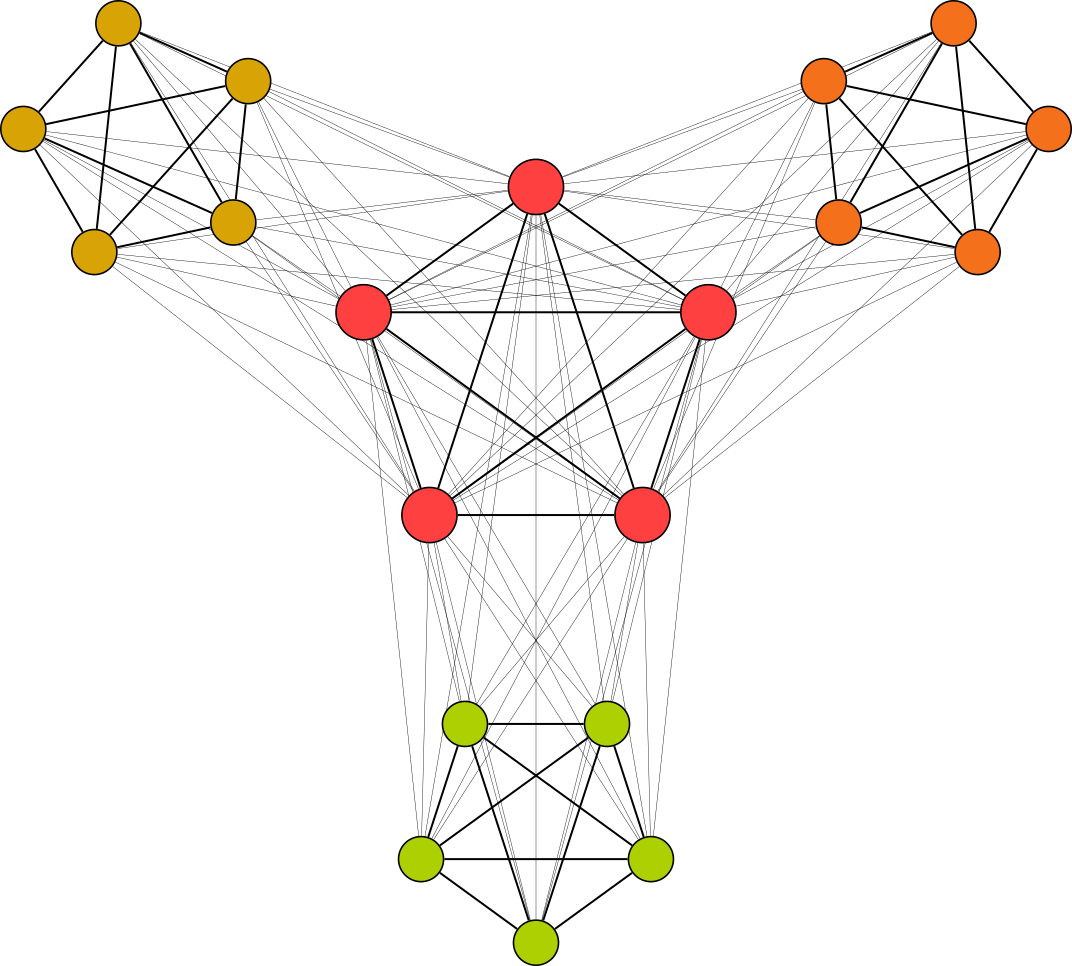
\includegraphics[max width=\linewidth, max height=\linewidth]{tiling_s5_d2_sag}
        \caption{2nd iteration. 10 tiles.}
        \label{fig:tree-tiling-v3-d2}
    \end{subfigure}%%
    \hfill
    \begin{subfigure}[m]{.32\textwidth}
        \vskip 0pt
        \centering
        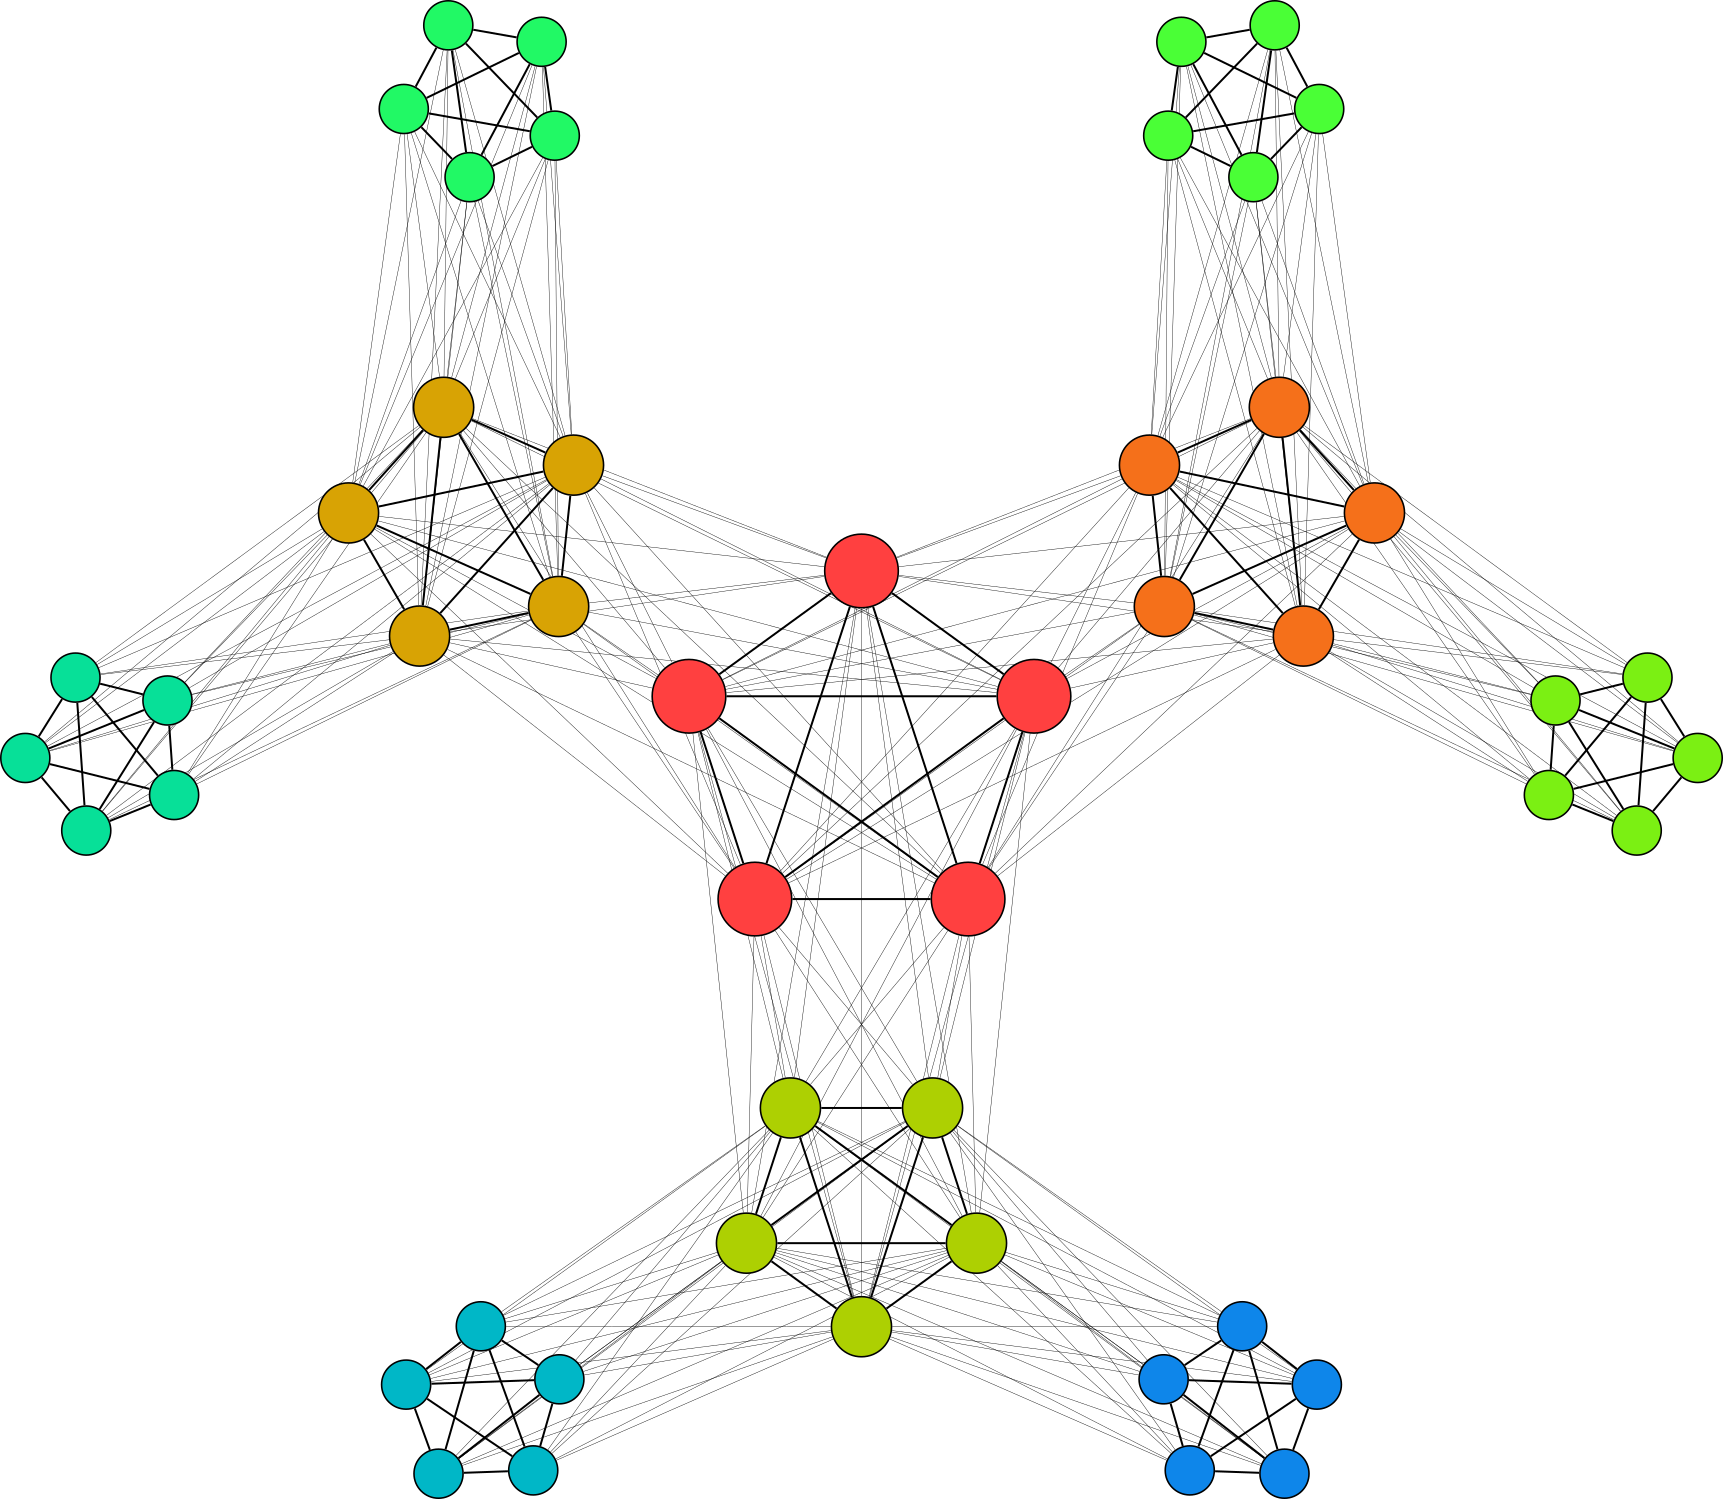
\includegraphics[max width=\linewidth, max height=\linewidth]{tiling_s5_d3_sag}
        \caption{3rd iteration. 22 tiles.}
        \label{fig:tree-tiling-v3-d3}
    \end{subfigure}
    \caption{}
    \label{fig:tree-tiling-v3}
\end{figure}

\subsubsubsection{\titlemath{$n$}{n}-ary Tree Tilings}

We will break our rules slightly: the root tile will have both twice the capacity for internal reflections than it would otherwise and one fewer children.
That is: the root tile reserves $2/v$ of it's capacity for reflections for internal reflections, instead of $1/v$ (as is the case for all other tiles), and it has $v-2$ children instead of $v-1$.
\autoref{fig:binary-tree-tiling} shows the first 3 iterations for $v=3$, and \autoref{fig:ternary-tree-tiling} shows the first 3 iterations for $v=4$.

\begin{figure}
    \begin{subfigure}[m]{.32\textwidth}
        \vskip 0pt
        \centering
        \includegraphics[max width=\linewidth, max height=\linewidth]{tiling_v3_nary_s5_d1_sag}
        \caption{1st iteration. 3 tiles.}
        \label{fig:binary-tree-tiling-d1}
    \end{subfigure}%%
    \hfill
    \begin{subfigure}[m]{.32\textwidth}
        \vskip 0pt
        \centering
        \includegraphics[max width=\linewidth, max height=\linewidth]{tiling_v3_nary_s5_d2_sag}
        \caption{2nd iteration. 7 tiles.}
        \label{fig:binary-tree-tiling-d2}
    \end{subfigure}%%
    \hfill
    \begin{subfigure}[m]{.32\textwidth}
        \vskip 0pt
        \centering
        \includegraphics[max width=\linewidth, max height=\linewidth]{tiling_v3_nary_s5_d3_sag}
        \caption{3rd iteration. 15 tiles.}
        \label{fig:binary-tree-tiling-d3}
    \end{subfigure}
    \caption{}
    \label{fig:binary-tree-tiling}
\end{figure}

\begin{figure}
    \begin{subfigure}[m]{.32\textwidth}
        \vskip 0pt
        \centering
        \includegraphics[max width=\linewidth, max height=\linewidth]{tiling_v4_nary_s5_d1_sag}
        \caption{1st iteration. 4 tiles.}
        \label{fig:ternary-tree-tiling-d1}
    \end{subfigure}%%
    \hfill
    \begin{subfigure}[m]{.32\textwidth}
        \vskip 0pt
        \centering
        \includegraphics[max width=\linewidth, max height=\linewidth]{tiling_v4_nary_s5_d2_sag}
        \caption{2nd iteration. 13 tiles.}
        \label{fig:ternary-tree-tiling-d2}
    \end{subfigure}%%
    \hfill
    \begin{subfigure}[m]{.32\textwidth}
        \vskip 0pt
        \centering
        \includegraphics[max width=\linewidth, max height=\linewidth]{tiling_v4_nary_s5_d3_sag}
        \caption{3rd iteration. 40 tiles.}
        \label{fig:ternary-tree-tiling-d3}
    \end{subfigure}
    \caption{}
    \label{fig:ternary-tree-tiling}
\end{figure}

\subsubsection{Tree Tilings: Preliminary Scaling Analysis}

\newpage


\subsubsection{Recursive \emph{Proof of Reflection}}

\mk{Maybe recursive PoR stuff should be moved to the PoR section, but that doesn't feel right b/c we don't use it before now (besides dapp-chains but that's trivial).}

\todo{edit start of this section to lead in from previous instead of being burried in Key Concepts}

Part of our security architecture will be the idea of \emph{recursive PoR}.

Say we have three chains: \cL, \cM, and \cR.
They are doing mutual reflection like this: $\xymatrix@C=1em@M=0em{{\cL} \; \ar@{<->}[r] & \; {\cM} \; \ar@{<->}[r] & \;{\cR}}$.
That is: \cL reflects \cM but not \cR; \cM reflects both \cL and \cR; and \cR reflects \cM but not \cL.

With what we already know, it's clear that \cM is as secure as all three combined.
However, that isn't the case for \cL and \cR.
How can we make \cL and \cR as secure as \cM?
Is this even reasonable?

Let's consider chain \cL -- what happens if \cL's local chain-work is, say, $3\times$ that of chain \cM?
The total chain-work that \cL takes into account is $\nicefrac43$ of its local chain-work, so an attacker would need $\nicefrac23$ worth of \cL's local chain-work to control \cL's history.
This is more than 50\%, but it's within reason that an attacker might achieve the required hash-rate.

Case 1: If \cR's local chain-work is large (say, $3\times$ that of \cM), then \cM is almost twice as hard to attack as \cL.\footnote{
    \cM is $\nicefrac74\times$ harder to attack than \cL.
}
This is a problematic situation: it means that an attacker might be able to perform a doublespend against \cL even though they could not perform one against \cM.
Therefore, this case would not be $O(n)$ secure.

Case 2: However, if \cR's local chain-work is small (say, $\nicefrac13$ that of \cM), then \cR is not particularly significant.
Thus, \cM is not substantially harder to attack than \cL, and an attacker could attack both \cL and \cM simultaneously (optionally, \cR too).
But, \cR \emph{is} substantially easier to attack than either \cM or \cL.
The total chain-work that \cR takes into account is only $\nicefrac4{13}$ that of the whole network.
So, this case is \emph{also} not $O(n)$ secure, even though \cL \emph{is} $O(n)$ secure.

These two problem cases are what recursive PoR solves.

Notice that in both cases, \cM is $O(n)$ secure.
Given this, chains \cL and \cR should be able to use the same work that chain \cM does to reach the same level of security.

The first problem is that \cL and \cR cannot use the same \textsc{WeightOf} algorithm as before (although, \cM can).
Particularly, \cL and \cR's \textsc{WeightOf} must count: not only their local chain-work and that contributed reflected \cM blocks, but also some additional weight based on reflections from \emph{other} chains.
Each \cM block might record the total chain-work that it adds to \cM (including PoRs), but \cL and \cR's new \textsc{WeightOf} can't use this value directly.
Firstly, that value includes past local chain-work that reflected \cM, but more importantly: we don't want to force \cL and \cR to verify \emph{every} PoR that contributes to \cM, just the ones that matter.
So how can \cL and \cR nodes know which work to count?

There is a trivial solution to this problem: require \cL and \cR nodes to download the headers of \emph{all} relevant chains, verify their PoRs, and track the origin of those PoRs.
Nodes must track the origin of work contributed via PoR to avoid double-counting work.
An easy example of this is: \cL nodes should not count PoRs where an \cL block is the reflecting block; that work is already directly included in \cL's local chain-work.

% commands used in the following xy chains diag

\providecommand\BL{}
\renewcommand\BL[1]{\BCI{\cL}{i}{#1}}
\newcommand\xBL[1]{\xyB{\BL{#1}}}

\providecommand\BR{}
\renewcommand\BR[1]{\BCI{\cR}{k}{#1}}
\newcommand\xBR[1]{\xyB{\BR{#1}}}

\providecommand\BM{}
\renewcommand\BM[1]{\BCI{\cM}{j}{#1}}
\newcommand\xBM[1]{\xyB{\BM{#1}}}

% ARrow reFlection
\newcommand\arf[1][]{\ar@{.>}[#1]}
\newcommand\arff[1][]{\ar@2{.>}@[Maroon][#1]}

Chain \cL can only count work contributed by \cR \emph{after} a multi-stage PoR can be constructed.
For example, let's consider the (rather orderly) chain-segments in \autoref{fig:simple-recursive-por-chain-diag}.

\begin{figure}
\begin{equation*}
    \xyMChains{
        \xyL{\text{Chain \cL}} & \cdots & \xBL1 \ar[l] & & \xBL2 \ar[ll] \arf[ld] & & \xBL3 \ar[ll] \arf[ld] \\
        \xyL{\text{Chain \cM}} & \cdots & & \xBM1 \ar[ll] \arf[ld] \arf[lu] & & \xBM2 \ar[ll] \arf[lu] \arf[ld] & \\
        \xyL{\text{Chain \cR}} & \cdots & \xBR1 \ar[l] & & \xBR2 \ar[ll] \arf[lu] & & \xBR3 \ar[ll] \arf[lu] \\
        \xyTimeHoriz{rrrrrr} &&&&&&
    }
\end{equation*}
\caption[
    asdf.
]{
    asdf.
}
\label{fig:simple-recursive-por-chain-diag}
\end{figure}

We can see that \BR{2} implicitly images \BL{1} via \BR{2}'s explicit imaging of \BM{1}.
This is because the network already depends on the PoRs that are sufficient to prove this. \BL{2}'s PoR for \BL{1} will prove $\xyInlineRefl{\BL{1}\;&\;\BM{1}\arf[l]}$ (i.e., that \BL{1} was imaged by \BM{1}).
\BM{2}'s PoR (via \cR) for \BM{1} will prove $\xyInlineRefl{\BM{1}\;&\;\BR{2}\arf[l]}$.

Similarly, we know that \BL{3} implicitly images \BR{2}: $\xyInlineRefl{\BR2\;&\;\BM2\arf[l]\;&\;\BL3\arf[l]}$.

Thus, for \BL3, we can construct a full PoR of \BL1 via \BR2 using the proofs for each link between them: $\xyInlineRefl{\BL1 \;&\; \BM{1}\arf[l] \;&\; \BR2\arf[l] \;&\; \BM2\arf[l] \;&\; \BL3\arf[l]}$.

Since \cL nodes already know about all the \cM and \cR blocks (and the relevant PoRs), the full recursive PoR \emph{does not need to be explicitly recorded}.
It is already known to all \cL nodes, since each part of the recursive PoR is available in one of the \cL, \cM, or \cR chains (it is explicitly recorded if a +PoRs UT variant is used, and recalculated by the node otherwise).

In \autoref{sec:counting-work} we discussed the idea that a PoR can only contribute to local blocks that are in the reflecting block's past.
By inspection, we can see that the most recent \cR block (the reflecting block) in \BL{3}'s past is \BR{2}, and the most recent \cL block (the local block) in \BR2's past is \BL1.
Thus, we can see that our method for attributing reflected work -- following the arrows -- works for recursive PoR, too.

There is something important to point out here: \emph{latency}.
Notice that these 4 blocks (in chronological order) are required for this recursive PoR to exist: \BM1, \BR2, \BM2, and \BL3.
This is twice the number of blocks that would normally be required without any recursion (e.g., a valid non-recursive PoR for \BL1 exists after \BM1 and then \BL2 are mined).
Therefore, the delay required for this PoR is twice what we would expect from non-recursive PoR.
In general (if only one PoR path between two given blocks will exist) this delay, measured in block periods, is the length of the full PoR.\footnote{
    For chains with equal block periods (and ignoring \emph{miner resonance}), there is a 50\% chance that chain \cR will produce a block before the next \cL block.

}

Recapping the first problem: \cL and \cR nodes need an expanded \textsc{WeightOf} function with access to \emph{the origin} of implicitly reflected work, and knowledge of \emph{where} that work has already been counted.
Nodes can do this relatively efficiently, for all relevant chains, by downloading the headers and verifying the PoRs.
This method does not require recursive PoRs to be explicitly recorded in full since the components of these PoRs are already available and have already been individually verified.
Our existing rules about how to attribute the weight of PoRs (follow the arrows) still works.

Our solution to the first problem is promising, but we have used an implicit assumption: there is only one viable path for PoRs between \cL and \cR.
What if there are \emph{multiple paths} between \cL and \cR?
This is the second problem.

\subsubsubsection{Recursive PoR with Multiple Paths}

\providecommand\BMone{}
\renewcommand\BMone[1]{\BCI{\cMone}{g}{#1}}
\newcommand\xBMone[1]{\xyB{\BMone{#1}}}

\providecommand\BMtwo{}
\renewcommand\BMtwo[1]{\BCI{\cMtwo}{h}{#1}}
\newcommand\xBMtwo[1]{\xyB{\BMtwo{#1}}}

% ARrow reFlection Bent Down
\newcommand\arfbd[1][]{\ar@{.>}@/_9pt/[#1]}
\newcommand\arfbu[1][]{\ar@{.>}@/^9pt/[#1]}

Say that we now have four chains: \cL, \cMone, \cMtwo, and \cR doing mutual PoR like so:
\begin{equation*}
    \xymatrix@C=2em@R=-.15em{
        & {\cMone}
        \ar@{<->}[dd]
        & \\
        {\cL} \ar@{<->}[ur] & & {\cR} \ar@{<->}[ul] \\
        & {\cMtwo} \ar@{<->}[ul] \ar@{<->}[ur] &
    }
\end{equation*}
Both \cMone and \cMtwo are already $O(n)$ secure.
Assuming that \cL and \cR nodes download and verify all PoRs, how can \cL and \cR count each other's work?

First, let's consider when \cL can \emph{definitely} count \emph{all} the work contributed by a \cR block.

\begin{figure}
    \begin{equation*}
        \xyMChains{
            \xyL{\text{Chain \cL}} & \cdots & \xBL1 \ar[l] & & \xBL2 \ar[ll] \arf[ld] \arfbu[ldd] & & \xBL3 \ar[ll] \arf[ld] \arfbu[ldd] \\
            \xyL{\text{Chain \cMone}} & \cdots & & \xBMone1 \ar[ll] \arfbd[ldd] \arf[lu] & & \xBMone2 \ar[ll] \arf[lu] \arfbd[ldd] & \\
            \xyL{\text{Chain \cMtwo}} & \cdots & & \xBMtwo1 \ar[ll] \arf[ld] \arfbu[luu] & & \xBMtwo2 \ar[ll] \arfbu[luu] \arf[ld] & \\
            \xyL{\text{Chain \cR}} & \cdots & \xBR1 \ar[l] & & \xBR2 \ar[ll] \arf[lu] \arfbd[luu] & & \xBR3 \ar[ll] \arf[lu] \arfbd[luu] \\
            \xyTimeHoriz{rrrrrr} &&&&&&
        }
    \end{equation*}
    \caption[
        asdf.
    ]{
        asdf.
        Note that reflections between \cMone and \cMtwo are not shown.
    }
    \label{fig:multi-path-recursive-por-chain-diag}
\end{figure}

As before, we'll look at valid PoRs for \BL3 that prove \BL1 was reflected in \BR2.
The exact reflections that exist will be analogous to our prior example, too.
See \autoref{fig:multi-path-recursive-por-chain-diag} for the chain-diagram.
% For each $x$ in $\{1,2,3\}$, we'll assume that \BL{x} and \BR{x} occur simultaneously, and both image \BMone{x-1} and \BMtwo{x-1}.
% After \BL{x}, but before \BL{x+1}, we'll assume that \BMone{x} and \BMtwo{x} are mined simultaneously and both blocks image \BL{x} and \BR{x}.
Notice that there are 4 possible paths from \BL{3} to \BL1:
% \\[-.66em]
\begin{equation*}
    \xymatrix@C=1em@R=-.5em{
        & & \BMone1 \arf[ld] & & \BMone2 \arf[ld] & \\
        \BL0 & \BL1 & & \BR2 \arf[lu] \arf[ld] & & \BL3 \arf[lu] \arf[ld] & \BL4 \\
        & & \BMtwo1 \arf[lu] & & \BMtwo2 \arf[lu] & \\
    }
\end{equation*}
% \\[-.66em]
Here is what we can say about this case: if all 4 of these PoR paths exist, then \BR2 \emph{definitely} reflects \BL1, and its weight can be included in \BL3's total chain-weight.

But, what if only some of those paths are available?
Consider this alternative case:
% hmm, unsure about the colors / focused arrows
\begin{equation*}
    \xymatrix@C=1em@R=-.15em{
        & \BMone1 \arff[ld] & & & \BMone2 \arf[llld] \arff[ld] & \\
        \BL0 & \BL1 & & \BR2 \arff[llu] \arff[ld] & & \BL3 \arff[lu] \arf[llld] & \BL4 \arf[ld] \\
        & & \BMtwo1 \arff[lu] & & & \BMtwo2 \arf[llu] \\
    }
\end{equation*}
In this case, \cL is implicitly reflected in \BR2, and \BL3 has two possible recursive PoRs of this (indicated via the double-lined arrows): \BL{1} via \BMtwo1; and \BL{0} via \BMone1.
Are both valid?
Is either preferable?
If \BL3 includes the full weight of \BR2 in its chain-weight, then what happens when \BL4 is mined and the other two PoR paths via \BMtwo2 become available?

We \emph{can} be sure that \BR2's weight can be fully included in \cL's chain-weight \emph{after} \BL4 is mined (as all PoR paths now exist).
However, it's not so clear what we should do when not all PoR paths yet exist.
Do we even need to solve this problem, now, though?

\begin{itemize}
    \item no -- it's enough to know that, when all PoR paths exist, the full weight is okay
    \item this is b/c we'll simplify tiles: every ${B_f}^{-1}$ seconds all chains in each tile mine 1 new block and provide reflections of 1 new block in their local tile and adjacent tiles, and vice versa.
    Thus all PoR paths are available all at once.
    \item we just need to be confident that an answer \emph{does} exist
    \item also, simplification case is much easier to reason about and solve for
    \item full solution left as a future research
    \item some ideas or questions for that future research:
    \begin{itemize}
        \item is a single PoR path enough to count the full weight of the reflecting block?
        \item if so -- tiling is very fast and secure. if not, tiling is pretty fast and still secure.
        \item what happens if some paths \emph{never} end up existing?
        \item do we divide contributed work by the number of paths?
        \item do paths have to go through the same chain? (i.e., $\cL \to \cMone \to \cR \to \cMone \to \cL$)
        \item can paths go through different chains? (i.e., $\cL \to \cMone \to \cR \to \cMtwo \to \cL$)
        \item should each PoR be valid if 1st and last entries are removed?
        if so, then it passes its weight to like that chain-segment (of the intermediate chain for which the middle bits of the recursive PoR are valid).
        \item but PoRs via different chains should still be valid b/c it shows order (thus we know that whatever's being reflected is in the history of every intermediate block)
        \item do we ever really need to consider this partial paths stuff?
        like a block (\BL3) that enables some PoR paths via a new block (\BR2) will probs also enable other missing PoR paths.
        Example: \BL4 enables \BR2 via \BMtwo2, but could also mb enable \BR3 via \BMtwo2, too.
        We should expect all paths to be available within a few block periods (e.g., $\sim 60$ s).
        \item WRT paths like $\cL \to \cMtwo \to \cMone \to \cR \to \cMone \to \cMtwo \to \cL$ (i.e., it's longer than the shortest path possible) -- we shouldn't need to count these.
        we should always be able to go directly b/c an implicit reflection in a chain's history that can also be explicit, should be explicit.
        so count these as 0 weight.
        \item idea: only the paths back matter. making more paths between the \cR block and most recent \cL block isn't so hard, but making the \cR block is (if the \cR block is relatively heavy, that is).
        So: divide \cR block weight by the number of \emph{paths back} and then only count unique shortest paths from $\BR{x} \to \BL{y}$.
        By that point, shouldn't \emph{all} those paths be available, anyway?
        \item maybe: path availability is only an issue between the reflecting \cR block and the current \cL block, but not between the \cR block and the reflected \cL block?
        (This sounds like it logically has to be true -- how could any new paths back be introduced!?)
        \item idea: the weights of all blocks in a recursive PoR path \emph{all} have the same \cL in their history, so their weights can be safely added to \cL.
        \item idea: the principle \emph{don't double-count work} means that when we have multiple paths back, that block's weight is attributable to the \emph{most recent} reflected \cL block.
        \item idea: the principle that \emph{a PoR is worth whatever is required to attack it} means that only 1 PoR path to the \cR block is required -- once that happens all other paths are redundant (though useful for SPV).
        \item idea: so the total weight contributed by a set of PoRs is the sum of all unique blocks in that set of PoRs -- multiple paths doesn't help.
        \item so simplex-chains in a deep tile get the security benefit of root tile chains as soon as a single path is available from an L block to any R block back to any L block.
        \item this should happen MUCH faster than the predicted delay between singularly reflected chains -- $v\cdot{N_1}^{-1}\times$ the duration, I think.
    \end{itemize}
    \item do miners need to be incentivized to reflect child chains?
\end{itemize}

There are some future areas of research that may improve this process, too.
For example: along the lines of NIPoPoWs\footnote{
    Non-Interactive Proofs of Proof-of-Work (NIPoPoWs), see \citeNIPoPoWsFull.
}, are \emph{Non-Interactive Proofs of Proof-of-Work Reflections} (NIPoPoWRs) possible?

\todo{por sim: are we double-counting reflections sometimes? should we divide the weight of a block by the number of local blocks that in reflects? what about blocks that have no explicit reflections? need to check sim logic.}

\todo{continue}

\subsubsubsection{Principles of PoR}

\begin{itemize}
    \item work can be converted to common units and thus summed
    \item work should not be double counted
    \item work is attributable to the most recent L block reflected by an R block (implies: pow's weight is transitive to all things in that PoWs history)
    \item work is work (law of identity; it means that it doesn't matter where/how work happens, just that it does and that its history includes the thing we want to prove)
\end{itemize}

\subsubsection{Tiling Security Stuff (Notes)}

\begin{itemize}
    \item self severance
    \item self sev + children
    \item sev child
\end{itemize}

\begin{itemize}
    \item floor((v-1)/2) = just less than half branches of root
    \item root + floor((v-1)/2) -- 50\% always
    \item
\end{itemize}

------

\begin{itemize}
    \item
\end{itemize}

\begin{forest}
    grow'=east,child anchor=west,
    for descendants={grow'=east,child anchor=west, align=center},
    [tiling security structure
     [analysis method
        [construction
            [tile-work]
            [$\text{Sec}(g|i)$ vs $w_{g|i}$]
            [$r$ and $s$]
            [$S {=} \sum_i w_i$]
        ]
     ]
     [evaluate cases
        [control tile \\ requires parent, align=center
            [don't need other cases]
            [below is stricter anyway]
        ]
        [root $> \frac{1}{2}S$, align=center]
        [$\frac{1}{2}$ (r + c) $> qS$, align=center]
        [$\frac{1}{2}$ (r + c + gc) $> qS$, align=center]
     ]
     [concessions
        [recursive PoR \\ validation, align=center
            [validate: \\ root + c + \\ ancestor tiles, align=center
                [$O(c \log(n))$]
            ]
            [problem: how \\ to count work?, align=center
                [sum of work can't \\ be > actual work]
            ]
        ]
     ]
    ]
\end{forest}

\subsubsection{Tree-Tiling Security}

\label{sec:tiling-security}

\todo{``Simplex Tile'' or ``Simplex-Tile''}

What does it mean for a tiling to be secure?
Well, we have our broad definition from the trilemma: the network is secure against an $O(n)$ attacker.
To answer this more specifically, though, we need to first answer: \emph{What does a doublespend against a tiling look like?}
Currently, we don't know enough to answer this -- we next need answers to questions like \emph{Which PoRs do simplex-chains in a given tile use?} and \emph{How do we govern the difficulties of simplex-chains in different tiles?}

To answer these questions, and then evaluate the security of tree-tiling, we first need to define some key concepts.
After that we will construct a security architecture so that we can answer the above questions.
Finally, we will analyze this architecture to find out if it's secure.

\subsubsubsection{Key Concepts}



\subsubsubsubsection{Local Chain-work, Tile-work, and Unit Tile}

We're familiar with \emph{local chain-work} (that's work directly contributed by a single simplex-chain).

\emph{Tile-work} is the work that is contributed from simplex-chains that are part of a given tile.
\emph{Tile-work} is the sum of the local chain-work of each constituent simplex-chain.

We could talk about tile-work directly in terms of \emph{number of hashes}, but this isn't necessary.
Instead, we'll normalize tile-work via a \emph{unit tile}.
If some tile's tile-work is $3\times$ that of the \emph{unit tile}, then we write down that tile-work as $3$ instead of some number of hashes.
This will simplify our analysis.

\subsubsubsubsection{The Core}

\emph{The core} of a tree-tiling is \emph{the root tile and its children}.
It's called \emph{the core} because all nodes in the network verify the work and PoRs of all simplex-chains that are part of the core.
Additionally, the core is where the vast majority of work is done.

\subsubsubsubsection{Recursive \emph{Proof of Reflection}}

\newcommand\cL{\ensuremath{L}\xspace}
\newcommand\cM{\ensuremath{M}\xspace}
\newcommand\cR{\ensuremath{R}\xspace}

Part of our security architecture will be the idea of \emph{recursive PoR}.

Say we have three chains: \cL, \cM, and \cR.
They are doing mutual reflection like this: $\xymatrix@C=1em@M=0em{{\cL} \; \ar@{<->}[r] & \; {\cM} \; \ar@{<->}[r] & \;{\cR}}$.
That is: \cL reflects \cM but not \cR; \cM reflects both \cL and \cR; and \cR reflects \cM but not \cL.

With what we already know, it's clear that \cM is as secure as all three combined.
However, that isn't the case for \cL and \cR.
How can we make \cL and \cR as secure as \cM?
Is this even reasonable?

Let's consider chain \cL -- what happens if \cL's local chain-work is, say, $3\times$ that of chain \cM?
The total chain-work that \cL takes into account is $\nicefrac43$ of its local chain-work, so an attacker would need $\nicefrac23$ worth of \cL's local chain-work to control \cL's history.
This is more than 50\%, but it's within reason that an attacker might achieve the required hash-rate.

Case 1: If \cR's local chain-work is large (say, $3\times$ that of \cM), then \cM is almost twice as hard to attack as \cL.\footnote{
    \cM is $\nicefrac74\times$ harder to attack than \cL.
}
This is a problematic situation: it means that an attacker might be able to perform a doublespend against \cL even though they could not perform one against \cM.
Therefore, this case would not be $O(n)$ secure.

Case 2: However, if \cR's local chain-work is small (say, $\nicefrac13$ that of \cM), then \cR is not particularly significant.
Thus, \cM is not substantially harder to attack than \cL, and an attacker could attack both \cL and \cM simultaneously (optionally, \cR too).
But, \cR \emph{is} substantially easier to attack than either \cM or \cL.
The total chain-work that \cR takes into account is only $\nicefrac4{13}$ that of the whole network.
So, this case is \emph{also} not $O(n)$ secure, even though \cL \emph{is} $O(n)$ secure.

These two problem cases are what recursive PoR solves.

Notice that in both cases, \cM is $O(n)$ secure.
Given this, chains \cL and \cR should be able to use the same work that chain \cM does to reach the same level of security.

The first problem is that \cL and \cR cannot use the same \textsc{WeightOf} algorithm as before (although, \cM can).
Particularly, \cL and \cR's \textsc{WeightOf} must count: not only their local chain-work and that contributed reflected \cM blocks, but also some additional weight based on reflections from \emph{other} chains.
Each \cM block might record the total chain-work that it adds to \cM (including PoRs), but \cL and \cR's new \textsc{WeightOf} can't use this value directly.
Firstly, that value includes past local chain-work that reflected \cM, but more importantly: we don't want to force \cL and \cR to verify \emph{every} PoR that contributes to \cM, just the ones that matter.

There is a trivial solution to this problem: require \cL and \cR nodes to download the headers of \emph{all} relevant chains, verify their PoRs, and track the origin of those PoRs.
Nodes must track the origin of work contributed via PoR to avoid double-counting work.
An easy example of this is: \cL nodes should not count PoRs where an \cL block is the reflecting block; that work is already directly included in \cL's local chain-work.
Another example is where there are \emph{multiple paths} that depend on the same chain.
This leads us into the second problem.

\subsubsubsubsection{Recursive PoR with Multiple Paths}

\newcommand\cMone{\ensuremath{M_1\xspace}}
\newcommand\cMtwo{\ensuremath{M_2\xspace}}

Say that we now have four chains: \cL, \cMone, \cMtwo, and \cR doing mutual PoR like so:
\begin{equation*}
    \xymatrix@C=2em@R=-.15em{
        & {\cMone} & \\
        {\cL} \ar@{<->}[ur] & & {\cR} \ar@{<->}[ul] \\
        & {\cMtwo} \ar@{<->}[ul] \ar@{<->}[ur] &
    }
\end{equation*}

\todo{continue}

\subsubsubsection{Security Architecture}

\subsubsubsubsection{Inter-tile Security Relationship}

$r$

\begin{forest}
    [ITSR
        [govern via RAA + DAA]
        [ratio of work based on $d$
            [$r$ \textrightarrow work drops by $1/r$ per layer]
        ]
        [root tile exception]
    ]
\end{forest}

\subsubsubsubsection{Total Work Across a Tiling}

$S$

\begin{itemize}
    \item Except for the root tile, each tile contributes $\frac1{r^d}$ work to the tiling.
    \item At each depth, there are $u^d$ tiles.
    \item Root tile contributes $M$ units of tile-work.
\end{itemize}

\begin{align}
    S &= M + \frac{u}{r} + \frac{u^2}{r^2} + \cdots && \text{Sum \emph{all} chain-work}
    \nonumber \\
    S - (M-1) &= 1 + \frac{u}{r} + \frac{u^2}{r^2} + \cdots
    \nonumber \\
    \intertext{This is a geometric series, and since $\frac{u}{r} < 1$:}
    S - (M-1) &= \frac{1}{1 - \frac{u}{r}} && \text{Sum of geometric series}
    \nonumber \\
    S - (M-1) &= \frac{r}{r - u} && \times\frac{r}r
    \nonumber \\
    S &= M-1 + \frac{r}{r - u}
    \label{eq:tree-tiling-total-work}
\end{align}

\subsubsubsubsection{Doublespend Requirements}

\subsubsubsection{Analysis Method}

How can we analyze the security of tree-tilings?


\subsubsubsection{Assumptions}

\begin{itemize}
    \item security of tile works like that of a simplex
    \item able to apply logic recursively
\end{itemize}

\subsubsubsection{Additional Imposed Requirements}

\subsubsubsection{Security Criteria for Specific Cases}

\subsubsubsection{Security Evaluation of Specific Cases}

\begin{itemize}
    \item $r>u$
    \item \dots
\end{itemize}

\subsubsubsubsection{The Core is (Almost) as Secure as the Network}

$M \ge 1$, $u > 1$, $r > u$, and $0 \le q \le 0.5$.

\begin{align}
    \frac12 (M + \frac{u}r) &> qS
    \nonumber \\
    \frac12 (Mr + u) &> rq(M-1+\frac{r}{r-u}) && \times r \text{ and substitute } S \text{ via \autoref{eq:tree-tiling-total-work}}
    \nonumber \\
    (Mr + u)(r-u) &> 2rq((M-1)(r-u)+r) && \times 2(r-u)
    \label{eq:tree-tiling-safe-q}
    % https://www.wolframalpha.com/input?i=%28My+%2B+x%29%28y-x%29+%3E+2yq%28%28M-1%29%28y-x%29%2By%29%2C+0+%3C%3D+q+%3C%3D+0.5
    % note for above: y=r; x=u
    % 2Mr &> |u| \sqrt{\frac{2M^2q-M^2-4Mq-2M+2q-1}{2q-1}}+u(M-1) \\
    % 2Mr &> |u| \sqrt{\frac{M^2(1 - 2q) - 2M(2q + 1) + (2q - 1)}{2q-1}}+u(M-1) \\
\end{align}

There is no elegant form of \autoref{eq:tree-tiling-safe-q}, but this form is, at least, easy to evaluate and graph.

\subsubsubsection{Scaling Complexity}

\subsubsubsubsection{Complexity of the Core}

\begin{forest}
    rectangle, draw=black, minimum width=6em, minimum height=1.5em,
    for descendants={rectangle, draw=black, minimum width=3em, minimum height=1.5em}
    [
        0,
        [0|0
            [0|0|0]
            [0|0|1]
        ]
        [0|1
            [0|1|0]
            [0|1|1]
        ]
    ]
\end{forest}

chains:

\begin{align*}
    N_\text{chains} &= N_{1,d=0} + 2N_{1,d=1} + 4N_{1,d=2} \\
    &= \frac{N_1}{4} + 2\frac{N_1}{4} + 4\frac{N_1}{4} \\
    &= \frac74 N_1 = O(c) \\
    \intertext{but if the core is just the root + children:}
    N_\text{chains} &= \frac34 N_1
\end{align*}

refls

\providecommand\parens[1]{%
{\left( #1 \right)}%
}
\providecommand\NOneSq{{{N_1}^2}}

\begin{align*}
    N_\text{refls} &= \left(\frac{N_1}{4}\right)^2 + 6\left( \frac{N_1}{4} \right)^2
                    + 2\left(\frac{N_1}{4}\cdot \frac{N_1}{4}\right)
                    + 4\left(\frac{N_1}{4}\right)^2 \\
    &= \NOneSq\parens{\frac{1}{16} + \frac{6}{16} + \frac{2}{16} + \frac{4}{16}} \\
    &= \frac{13}{16}\NOneSq = O(c^2) \\
    \intertext{but if the core is just the root + children:}
    N_\text{refls} &= \parens{\frac{N_1}{4}}^2 + 2\parens{\frac{N_1}{4}}^2 + 2\parens{\frac{N_1}{4}\cdot \frac{N_1}{4}} \\
    &= \frac{5}{16}\NOneSq
\end{align*}

for a leaf tile, each layer adds $2\parens{\frac{N_1}{4}}^2$ more reflections, so we get $\ceil{8 (1 - \frac5{16})}-1 = 5$ layers for free.

\begin{align*}
    2^2 - 1 &\to 2^{2+5} - 1 \\
    &\implies \frac{2^7 - 1}{3}\times \text{ the capacity.} \\
    &\approx 42\times
\end{align*}

\begin{equation*}
    a
\end{equation*}

\subsubsubsubsection{Security Burden Complexity}

each tile has a local $O(c)$ load for PoR verification

each tile is $h \lesssim \log_2(n)$ away from the root

all tiles between that tile and the root need to have PoRs verified, plus the root and its surrounding tiles, and the local tile's neighbors.

root + children + gc + in-between + local + children

$R = \text{root} = 2$

that's $((v-1)^2 + (v-1) + R) + \max(0, h - 3) + (1 + (v-1))$

\begin{align*}
    & & &\quad\:\: ((v-1)^2 + (v-1) + R) + \max(0, h - 3) + (1 + (v-1)) \\
    & & &= (v^2 - 2v - 1 + v - 1 + 2) + \max(0, h - 3) + v \\
    & & &= v^2 + \max(0, h-3) \\
    & & &= O(v^2) + O(\max(0, h-3)) \\
    & & &= O(v^2) + O(h) \\
    & & &= O(v^2) + O(\log(n)) \\
    & & &= O(v^2 + \log(n)) \\
    \text{since } v^2 \text{ is constant:} & & &= O(\log(n)) \\
    % \therefore \text{ (assuming +PoRs) total load is:} & & & O(c\log(n)) \\
    \therefore \text{ total load is:} & & & O(c^2\log(n)) \\
\end{align*}

\subsubsubsubsection{Capacity Complexity}

\begin{center}
\begin{forest}
    [Root
        [c1
            [c11]
            [c12]
        ]
        [c2
            [c21]
            [c22]
        ]
    ]
\end{forest}
\end{center}

\begin{align*}
    N_\text{tiles} &= \frac{u^{h+1} - 1}{u-1} \\
    &= O(u^h) = O(n)
\end{align*}

\begin{align*}
    2^{44} &> r^{h} \\
    44 &> h \log_2(r) \\
    \frac{44}{\log_2(r)} &> h \\
    \intertext{$r' \ge r$, so:}
    \frac{44}{\log_2(r)} \ge \frac{44}{\log_2(r')} &> h \\
    \frac{44}{\log_2(5)} &> h \\
    \sim 19 &> h \\
    \implies N_\text{tiles} &\lesssim 2^{19} \approx 5\cdot 10^{5} \\
    \intertext{if 96 bits are available:}
    \sim 41 &> h \\
    \implies N_\text{tiles} &\lesssim 2^{41} \approx 2\cdot 10^{12} \\
\end{align*}

\subsubsection{Asymmetry: Capacity and Security}

% https://www.desmos.com/calculator/7trq5aehnm
% https://www.desmos.com/calculator/n17w3560ig

\todo{why do $n$-ary tree-tilings?}

\subsubsection{future work}

\begin{forest}
    for descendants={align=center,},
    [future work
        [NIPoPoWRs
            [very concise \\ PoRs at depth?]
        ]
        [better tiling patterns
            [parameters
                [valence]
                [$r$]
            ]
            [designs
                [e.g.\, n-ary trees improved \\ over maximal trees]
            ]
        ]
    ]
\end{forest}



%
% The in-prog doc we want to preview
%

% \aside{
    Don't you think it's time for an epigraph?
}

\wideepigraph

\epigraph{
    Nobody stays in this valley except by a full, conscious choice based on a full, conscious knowledge of every fact involved in his decision. Nobody stays here by faking reality in any manner whatever.
}{Ayn Rand (Atlas Shrugged)}

\aside{
    Or, perhaps you might prefer something from Karl Popper?
    Very well:
}

\epigraph{
    On the level of scientific discovery two new aspects emerge. The most important one is that scientific theories can be formulated linguistically, and that they can even be published. Thus they become objects outside of ourselves: objects open to investigation. As a consequence, they are now open to \emph{criticism}. Thus we can get rid of a badly fitting theory before the adoption of the theory makes us unfit to survive. \emph{By criticizing our theories we can let our theories die in our stead.} This is of course immensely important.
}{Karl Popper (The Myth of the Framework)}

\aside{
    Let's proceed.
}

\subsubsubsection{Simplex Security}

\label{sec:simplex-security}

Simplexes are secure if attacking a single simplex-chain is as difficult as attacking the whole simplex (the network).

Say the attacker controls $q$ proportion of the network's work-generation capacity (e.g., hash-rate for PoW chains), and honest nodes control $p$ proportion, such that $p+q=1$.
The attacker should only be able to perform a doublespend if $q > p$.

Successfully attacking a single blockchain requires an attacker to publish an alternate chain-segment that the fork rule considers heavier than the corresponding public chain-segment.
Those two segments will have a common ancestor, so the weight of the attacker's segment must be greater than the weight of the public chain-segment (from that common ancestor on).

Simplex-chains evaluate block-weight as the sum of work done on that block, plus work done on reflecting blocks.
So effecting a doublespend on one simplex-chain requires generating a chain-segment with more total block-weight (including reflections) than the public chain-segment.

It is not viable for the attacker to mine the attacking chain-segment in public (see \autoref{sec:dos-and-dags}), so they must mine it in private.
Blocks mined in private will not gain reflections from honest miners on other simplex-chains, so any reflections contributing to the doublespend must be created by the attacker.
The attacker's reflecting blocks (which reflect the attacking chain-segment) on other simplex-chains can be public, but the attacker's task is simpler and not detectable if the attacker mines reflecting blocks in private.\footnote{
    Additionally, if reflecting chains maintain projections as headers-only chains (i.e., construct a main chain via SPV rules), then it should be much harder for an attacker to succeed if reflections are mined in public.
}
There is no viable way for the attacker to prevent honest miners from reflecting the honest chain-segment, including new blocks that extend it, nor to prevent the honest chain-segment from reflecting blocks from other simplex-chains (again, see \autoref{sec:dos-and-dags}).

The honest chain-segment, on the targeted simplex-chain, will not be reflected by the attacker (since that would be self-defeating).
Similarly, the attacker's chain-segment will not be reflected by the honest network, since it's being mined in private.

\todo{need to add some stuff in here -- a bit more explanation and linking, particularly consider editing 'it is not viable' paragraph}

Let $r$ be the network-wide rate-of-work (hash-rate).
Over some attack duration $d$, we expect the attacker's chain-segment to weigh $qrd$, and the honest chain-segment to weigh $prd$.
Thus, for the attacker's chain-segment to win, it must be that $qrd > prd \implies q > p$.
$\blacksquare$

\subsubsubsection{Confirmation Equivalence Conjecture}

\defineTerm{Confirmation Equivalence Conjecture (CEC)}{
    The conjecture that, when using PoR and appropriately converting work,
    confirmations of reflecting chains
    can be treated as \emph{equivalent} to local confirmations of the same weight
}

The Confirmation Equivalence Conjecture is why PoR works.
If it were false, then PoR could not work, and neither would simplexes.
Additionally, this is the root of UT's $O(c)$ confirmation rate -- the conjecture implies that confirmation rate is proportional to the number of mutually reflecting chains.

Can we test it? If so, how?

Consider a traditional PoW blockchain (e.g., Bitcoin, Eth1, etc).
It's well known that the risk of a doublespend against a particular block is related to the number of \emph{confirmations} that block has.\footnote{
    See \href{https://web.archive.org/web/20220209100515/https://cloudflare-ipfs.com/ipfs/QmNUWmY94QUievK8ptoxsPyAQUsKvx1cjRyCgPcfmysAVv}{Analysis of hashrate-based double-spending}.
}
However, this is not a linear relationship; rather, it's similar to \emph{exponential decay}.
After the first few confirmations, each additional confirmation reduces the risk of a doublespend by approximately the same factor.\footnote{
    The exact factor depends on the attacker's hash-rate as a proportion of the network's (i.e., $q$).
}
So \emph{security takes \textbf{time}}, because confirmations take time.

Now, consider a simplex: the equivalence conjecture says that it doesn't matter whether confirmations come from the \emph{local} chain, or if they come from a \emph{reflecting} chain.
So, a simplex-chain in a 2-chain simplex (wherein each simplex-chain has $\mathbb{C}^\prime = 2 \times B_f$) \emph{should}, after $C$ confirmations, be as secure as a standalone blockchain with $2C$ confirmations.
Or, more generally, a simplex-chain in an $N$-chain simplex will, after $C$ \emph{local} confirmations, be as secure as a standalone blockchain after $NC$ confirmations.

This is something we can test!
(See \autoref{sec:por-simulation-results} for that.)

As blockchain architects, if the CEC is true, then UT allows us to maintain security by trading \emph{waiting time} for \emph{more simplex-chains!}

\aside{
    If you were looking for an essence of how UT breaks the core conflict of Buterin's Trilemma\dots
}

\subsubsubsection{Generalizing Doublespends}

With a traditional blockchain, the network has no "memory" of work (hashes) that have been done but are not accounted for in the main chain.
Specifically, the network gains no knowledge of how much work has been done \emph{between} block.
This is almost self-evident: each block is the \emph{sole} way that work can be \emph{added} to the chain.
Naturally, there is no smaller unit of contributed work than an individual block -- so there's no "memory".\footnote{
    We're not concerned with things like \emph{weak blocks} or super-block hybrid designs; though it's possible that doublespend methodology for those designs has some overlap with this section.
}

When an attacker publishes a heavier chain-segment which causes a reorganization, it is \emph{immediately} in the interests of miners to begin building on the attacker's best block.
A heavier chain-segment is \emph{decisively better} in all cases.
That may seem so obvious that it isn't worth mentioning, but it's actually a \emph{specific case} that only works for traditional blockchains.
If there were some "memory", it might be worth miners \emph{continuing} mining their \emph{existing} block, \emph{instead} of reorganizing and building on the attacker's best block.

What kind of "memory" could there be?
Are \emph{Proofs of Reflection} a "memory"?

As it turns out: yes.

Let the total chain-weight of the attacker's best block be called $W_A$, and the total chain-weight of the honest network's best block be called $W_H$.

Consider a miner of a simplex-chain (chain $L$) who is working on a \emph{draft block} during an active attack (though, of course, the miner does not know that).
Specifically, let's consider \emph{just before} the attacker publishes their chain-segment.
In the memory pool\footnote{
  The \emph{memory pool} is where unconfirmed transactions (and other things) are stored before they are included in a block.
  Each node has their own memory pool -- this must be the case because securely synchronizing memory pools between untrusted parties is as difficult as running a whole blockchain.
  A miner typically decides a block's contents by choosing the combination of transactions from their memory pool that results in the largest reward (i.e., transactions with the largest fees).
} of that miner, there will be PoRs, and those PoRs are \emph{only} valid for the \emph{honest} chain-segment (most likely they are for the best known honest block, but don't need to be).
Each $L$ block, in and of itself, only adds $\sim w$ weight to the $L$ chain.
However, if that \emph{draft block} contains $\sim n$ pending PoRs, and each PoR provides $\sim w$ weight on average, then a valid block (created from that draft) will contribute, via PoRs, $\sim nw$ weight to the \emph{honest chain-segment}.
Thus, the miner has this choice: reorganize to the attacker's chain-segment and mine on top of a chain with weight $W_A$, \emph{or} continue mining on the honest chain-segment that weighs $W_H + nw$.

The $nw$ term is that "memory", and it makes all the difference.
Only when $W_A > W_H + nw$ is it safe for an attacker to publish their chain-segment -- then it is \emph{decisively better} than the honest chain-segment.
If, however, the attacker publishes their chain-segment when $W_H < W_A < W_H + nw$: the best chain-segment for honest miners to mine is \emph{still} the honest chain-segment, not the attacker's!

Miners don't actually have to change their behavior at all: their choice is the same, whether they are mining a simplex-chain \emph{or} a traditional chain.
That choice is: \emph{of all possible blocks to mine, which results in the greatest reward?}
If they build on the honest chain-segment, does their resulting block have more total chain-weight than if they were to build on the attacker's chain-segment?

There are some subtleties to consider if chains are DAGs or use GHOST: both chain-segments can be included as ancestors, but which should take priority?
If the weight of PoRs is not taken into account (or applied after evaluating the order of parents), then the attacker's chain-segment takes priority when $W_A > W_H$.
This rule conflicts with what we discussed above, so it must be that parents are ordered based on their chain-weights \emph{including} any PoRs in that block -- the honest chain-segment should take priority when $W_A < W_H + nw$.
Also, note that this is why the weight of PoRs is attributed to the \emph{reflected} block (usually a parent) rather than the block that contains the PoRs.
In essence, the inclusion of this "memory" requires that the fork rule take \emph{context} into account -- particularly the context of the descendant block.
This is not a paradox because the fork rule is \emph{only} used to choose the priority chain in the context of some descendant block (even if that block is an invalid draft).

\subsubsubsection{Testing the Confirmation Equivalence Conjecture}

\label{sec:por-simulation-results}

Let's test the Confirmation Equivalence Conjecture.

\subsubsubsubsection{Hypothesis}

The hypothesis is that: doublespends against an \emph{individual simplex-chain} in an $N$-chain simplex after $C$ \emph{local} confirmations are \emph{as hard} as doublespends against a traditional blockchain after $N\cdot C$ confirmations.

Define $P(N_1 = N; c = C; q = Q)$ (for some given $N$, $C$, and $Q$) to be the probability of an attack succeeding after $c$ confirmations against a simplex with $N_1$ simplex-chains, given an attacker with $q$ proportion of the network hash-rate.

Note that a simplex of 1 chain (the 0-simplex) \emph{is} a traditional blockchain.
So we can take Bitcoin for example: the probability of an attack succeeding after 6 confirmations is given by $P(N_1 = 1; c = 6; q = Q)$ -- of course, we still need to know the attacker's hash-rate to calculate this.

Thus, the hypothesis is that:
\begin{equation}
    P(N_1 = N; c = C; q = Q) \approx P(N_1 = 1; c = NC; q = Q)
    \label{eq:por-sim-hypothesis}
\end{equation}

\subsubsubsubsection{Method}

I have implemented a model blockchain network with attack simulations wherein each chain uses PoW and has a fully functioning fork rule.
This design is modular, such that it supports different fork rules, different block data structures and ordering algorithms (including multiple parents), different attack strategies.
The program also accepts a variety of parameters -- both for the simulation itself, the individual chains, and for each attack strategy.

The source code for this model blockchain network is contained in the \href{https://github.com/AmarooHQ/whitepaper/tree/master/experiments/por-sim-rs}{\texttt{/experiments/por-sim-rs/}} folder of \href{https://github.com/AmarooHQ/whitepaper}{this paper's repository}.

As we can optimize this model, we can simulate many attacks quickly; so we can efficiently make statistically significant measurements.

\todo{asdf - continue method}

\subsubsubsubsection{Scope and Constraints}

This experiment is not intended to be comprehensive -- many significant real-world factors are basically ignored: e.g., block propagation latency, transaction processing overhead, geographic latency, bandwidth constraints, etc.

The scope is \emph{only} intended to cover PoR as a consensus mechanism -- particularly with respect to doublespends.

This constraint means there are many ways to simplify implementation -- for example, reflected blocks are not checked against the history of a blockchain.
These simplifications would render a \emph{production} blockchain insecure.
However, the simplifications are okay in this case since we \emph{expect} near-identical behavior from well functioning networks, and the simplifications are otherwise independent of what we are testing -- the consensus mechanism.
In essence, we want to simulate a \emph{specific} attack, so the implementation doesn't need to be hardened because we know that the attacker will \emph{only} attack in the specific way we care about.

So, while it is \emph{possible} that a poor implementation of a simplex could compromise its security, we'll assume these kinds of design flaws are \emph{in principle} avoidable.

\todoDraftOnly{Test chains of different hash-rates + anything else to cover bases re CEC}

\subsubsubsubsection{Interpreting the Results}

\todo{por sim - Interpreting the Results}

\subsubsubsubsection{Results}

\todo{por sim results}

\subsubsubsubsection{Discussion}

\todo{por sim discussion}

\subsubsubsubsection{Experimental Limitations}

\todo{por sim - limits}

* could be insecure for reasons we didn't test for
* those ignored factors could be decisive
* insufficient breadth of attack parameters
* didn't come up with a good strategy (mb there's a better one than mining in private)
* confirmation bias in implementation -- might have missed something
* does it work for simplexes that have PoS/PoA chains? not tested for

% \todoDraftOnly{Revisit counting work section in a bit and mb redraft}

\todoDraftOnly{review all of 3.1 for references to PoRs only providing weight to the best block, etc. (this was an old idea and is not the case.)}

\providecommand\BL[1]{\BCI{L}{i}{#1}}
\providecommand\BR[1]{\BCI{R}{j}{#1}}
% note: \BR renewed below to change `j` term to `k`

When chains L and R have the same block frequency and produce blocks in an orderly fashion, it's trivial to count how much work is contributed by each PoR.
However, real-world blockchains do not produce blocks like this --- even if chains L and R have the same block frequencies, sometimes L will produce 2 or 3 (or more) blocks before R produces its next one (or vice versa).
\begin{equation*}
    \xyMChains{
        \xyL{\text{Chain L}} & \cdots & \xyB{L_i} \ar[l] & & \xyB{L_{i+1}} \ar[ll] \ar@{.>}[ld] & \xyB{L_{i+2}} \ar[l] & \xyB{L_{i+3}} \ar[l] & \\
        \xyL{\text{Chain R}} & \cdots & & \xyB{R_k} \ar[ll] \ar@{.>}[lu] & & & & \xyB{R_{k+1}} \ar[llll] \ar@{.>}[lu] \\
        \xyTimeHoriz{rrrrrrr} & & & & & & & \\
    }
\end{equation*}
Should \BR{1} include 3 PoRs, or just 1?
How should \BR{1} calculate the weight of those PoRs and the total weight contributed to chain R?

If \BR{1} had reflected only \BL{1}, then it's clear that we would count work from both \BL{1} and \BR{1} --- that much is easy.
However, \BR{1} reflected \emph{three} L headers.
Should \BR{1} count work from \emph{all three}, or something else?
Why?

Consider the situation from the miner's perspective (the miner of \BL{2}).
There is no new R block for them to reflect --- if there were, they'd include it.
The miner is effectively claiming --- via the absence of a new reflection --- that \BL{2}'s parent (\BL{1}) reflects the most recent R header ($R_k$); that \BL{1} is still \emph{up-to-date}.
From this perspective, it's clear that \BL{2} should contribute reflected weight to the best R headers that were most recently reflected: in this case, just $R_k$.

We can evaluate \BL{3} the same way.

So, yes \BR{1} should include and count work from all 3 PoRs in this case.

\providecommand\BRj[1]{\BCI{R}{j}{#1}}
\renewcommand\BR[1]{\BCI{R}{k}{#1}}

What about a more complicated example?
\begin{equation*}
    \xyMChains{
        \xyL{\text{Chain L}} & \cdots & \xyB{L_i} \ar[l] & & \xyB{L_{i+1}} \ar[ll] \ar@{.>}[ld] & \xyB{L_{i+2}} \ar[l] & \xyB{L_{i+3}} \ar[l] & & \xyB{L_{i+4}} \ar[ll] \ar@{.>}[ld] \\
        \xyL{\text{Chain R}} & \cdots & & \xyB{R_k} \ar[ll] \ar@{.>}[lu] & & \xyB{R_{k+1}} \ar[ll] & & \xyB{R_{k+2}} \ar[ll] \ar@{.>}[lu] & \\
        \xyTimeHoriz{rrrrrrrr} & & & & & & & & \\
    }
\end{equation*}
\BR{2} can be evaluated by similar logic to \BRj{1} above, but what about \BL{4}?

Does \BL{4} count the weight of \BR{1}?
If so, does it count towards \BL{3}'s chain-weight?

The difficulty in answering these questions --- with what we've covered so far --- is that \emph{the fork-rule doesn't care} where the weight is added, just that it \emph{is} added.
When the fork rule compares \BL{4} to an alternative block, only the \emph{total} chain-weight of each is relevant.
However, to understand exactly how PoRs \emph{should} be counted, we need to know more.

The essence of PoR is \emph{the confirmation of another chain's \ul{history}} --- so a reflection cannot contribute to a block which exists \emph{in the reflecting block's \ul{future}}.
It must be that reflections contribute to the \emph{most recent common ancestor} of all \emph{possible} L blocks which \emph{could} include that specific PoR.

This leads us to a simple and elegant way to count reflected work: follow the arrows back from the reflecting block to the most recently reflected local block.

\BL{4}'s reflection of \BR{2} contributes chain-weight to \BL{3} because \emph{any} block that builds on \BL{3} could reflect \BR{2}.
% (L_{i+4} \; \ar@{.>}[r] &) \;
Following the arrows: $\xyInlineRefl{R_{k+2} \; \ar@{.>}[r] & \; L_{i+3}}$.
% Note that the blocks and links in parentheses are specific to the block

% Following the arrows: $L_{i+4} \dashrightarrow R_{k+2} \dashrightarrow L_{i+3}$.

Similarly, \BL{4}'s reflection of \BR{1} (which could be either explicit or implicit via \BR{2}) must contribute chain-weight to $L_i$ because \emph{any} block building on $L_i$ could reflect \BR{1} and include that PoR.
% (L_{i+4} \; \ar@{.>}[r] & \; R_{k+2} \; \ar[r] &) \;
Following the arrows: $\xyInlineRefl{R_{k+1} \; \ar[r] & \; R_k \; \ar@{.>}[r] & \; L_{i}}$.

% \BL{4} \textrightarrow \BR{2} \textrightarrow \BR{1} \textrightarrow $R_k$ \textrightarrow $L_i$.
% Following the arrows: $L_{i+4} \dashrightarrow R_{k+2} \to R_{k+1} \to R_k \dashrightarrow L_{i}$.

We can also say more about \BR{2}'s reflection of \BL{3}, now, too.
Particularly, that the reflected work of $\BL{1}\cdots \BL{3}$ should contribute to \BR{}, \emph{not} \BR{1}.

\begin{draftonly}

\todoDraftOnly{subsubsec counting work extra}

\todoDraftOnly{
consider a situation where an attacker reflects 1 honest block and 1 competing attacker block, and the attacker block is not released.
for the sake of the argument, assume the reflected blocks weight much less than the reflecting block.
}


\todoDraftOnly{
    consensus enforces availability of refl blocks
    but counting work doesn't know anything about 'availability'
    so the only thing it can do is know if something is within its history or not.
    asymmetry.
}

\todo{
    noncontributing pors: like ghost (uncles) for PoR --- reflection isn't 2 ways?
    is this okay with miner incentives? or is there a conflict?
}

\end{draftonly}


\end{section}

\appendix

% \section{CEC Experiment Extra}

\label{sec:appendix-cec-extra}

\subsection{Results with $q = 0.48$}

\autoref{fig:cec-48-results} shows results of the simulation for $q=0.48$.
Unlike earlier figures, this figure uses $c = 20$ as the basis for comparison instead of $c = 5$ to accommodate the extended duration of attacks performed by an attacker close to 50\% of the global hash-rate.
These results do converge as predicted by the CEC, but not as closely as the results in \autoref{sec:por-simulation-experiment}.

\begin{figure}[H]
    \centering
    
\includegraphics[max width=\linewidth, max height=0.33\textheight]{simulation/_results_extra_q=0.48_daa=500_nofrac.pdf}
    \caption[]{
        Main results for $q=0.48$ for the experiment documented in \autoref{sec:por-simulation-experiment}
    }
    \label{fig:cec-48-results}
\end{figure}

\subsection{Simulator Iteration}

\todoDraftOnly{add captions and discussion}

\subsubsection{Initial Results}

\begin{figure}[H]
    \centering
    
\includegraphics[max width=\linewidth, max height=0.33\textheight]{simulation/lp_early_results.pdf}
    \caption[]{
    }
    \label{fig:cec-extra-first-res}
\end{figure}

% \subsubsection{Doublespends on Traditional Chains and DAAs}

\subsubsection{Accounting for Draft Reflecting Work}

\begin{figure}[H]
    \centering
    
\includegraphics[max width=\linewidth, max height=0.33\textheight]{simulation/lp_results_after_draft_refl_work.pdf}
    \caption[]{
    }
    \label{fig:cec-extra-draft-refl-work}
\end{figure}

\subsubsection{Attacker's Hash Rate Distribution: Uniform vs Random}

\begin{figure}[H]
    \centering
    
\includegraphics[max width=\linewidth, max height=0.33\textheight]{simulation/_interim_randhr.pdf}
    \caption[]{
    }
    \label{fig:cec-extra-randhr}
\end{figure}

\subsubsection{The Attacker's ``Bonus Block''}

\begin{figure}[H]
    \centering
    
\includegraphics[max width=\linewidth, max height=0.33\textheight]{simulation/_interim_bonusblock.pdf}
    \caption[]{
    }
    \label{fig:cec-extra-bonusblock}
\end{figure}

\subsubsection{Effects of $\text{DAA}_N$}

\begin{figure}[H]
    \centering
    
\includegraphics[max width=\linewidth, max height=0.33\textheight]{simulation/_interim_daa.pdf}
    \caption[]{
    }
    \label{fig:cec-extra-daa}
\end{figure}


\end{document}
